%make the document class option "PhD,final" to remove todo list items
\documentclass[PhD]{msu-thesis}


% Your extra packages here
%
\usepackage{graphicx}
\usepackage[colorlinks=true, citecolor=black, linkcolor=black, urlcolor=blue]{hyperref}
\usepackage{array,multirow}
\usepackage{tabularx}
\usepackage{hhline}
\usepackage{makecell}
\usepackage[obeyFinal,colorinlistoftodos]{todonotes}
\usepackage{courier}
%\usepackage[toc,page]{appendix}
\renewcommand\theadalign{cb}
\renewcommand\theadfont{\bfseries}

%\presetkeys{todonotes}{color=yellow!30, inline}{}
%

%newcommand{\todo[color=red]}[2][]
%{\todo[color=red, #1]{#2}}

%newcommand{\todo[color=green]}[2][]
%{\todo[color=green, #1]{#2}}

\makeatletter
\g@addto@macro\@floatboxreset\centering
\makeatother


% Define the title, author, field of study, date, and dedication (optional)
%
\title{Evolution and Evolvability in Changing Environments}
\author{Rosangela Canino-Koning}
\fieldofstudy{Computer Science} % should be in sentence case
\dedication{This thesis is dedicated to Kendall Koning.}
\date{2017}
%
\begin{document}
\frontmatter
%
\maketitlepage
%

\begin{abstract}
\todo[inline]{prep a layman's abstract if I have time}
\todo[inline, color=magenta]{rework abstract}
% The specific meaning of the term ``evolvability'' is heavily debated, but most definitions can be summarized as: the potential of populations and genomes to produce adaptive variation and complex structures in response to mutation and selection. Evolvability is thought to be created through the interplay of modularity and robustness. Indeed, modularity and robustness build upon each other, layer by layer, to form a framework that produces more powerful adaptive effects while reducing the impact of deleterious mutations.

% In this comprehensive exam, I will describe some research that I have completed and propose additional projects that explore the interplay among evolvability, robustness, and modularity. Before delving into my own research, however, I begin in the first chapter by providing a survey of current literature on each of these topics, with emphases on how they are believed to arise, how they affect subsequent evolution, and how they relate to each other.

% Modularity and robustness clearly have a complex interdependence in ongoing evolutionary dynamics, but they can evolve via simple mechanisms that are a byproduct of direct selection on other traits. Specifically, more modular and more robust genetic architectures are more likely to produce successful phenotypes, and thus they hitchhike to fixation in the population. In Chapter 2, I demonstrate how a cyclically changing environment provides a sufficient selective pressure to produce quasi-modular genetic architectures, independent of other features.

% In the third chapter, I propose to study how modularity might also arise as a result of horizontal gene transfer. We hypothesize that organisms will choose to uptake gene fragments for food, even when there is a chance that those fragments might be integrated into the genome. Furthermore, we expect that this uptake will result in higher modularity and, in turn, evolvability over time.

% In Chapter 4, I propose to study how modularity and robustness affect the character of the local mutational landscape around evolved organisms. We hypothesize that populations made up of organisms possessing a robust phenotype will not only display more genomic diversity within that phenotype (since so many mutational possibilities will arrive back to the same phenotype), but the non-neutral mutants appearing in that population will display greater variety of distinct phenotypes as well. 

% In the fifth chapter, we show that sexual selection facilitates speciation through reduced gene-flow across groups. Specifically, we demonstrate that sexual selection is a strong early facilitator of reproductive isolation, and that post-zygotic isolation is not required to reduce gene flow between populations. Thus, sexual selection may aid in the fixation of evolvable traits in isolated populations.

% In the final chapter, I conclude with a project plan, including a timeline for completion of the remaining experiments.
\end{abstract}
%
\clearpage
\makecopyrightpage
\makededicationpage
%
\clearpage
\chapter*{Acknowledgments}
\DoubleSpacing
Your acknowledgments here
\todo{acknowledgments}
%
\clearpage
\SingleSpacing
\tableofcontents*
\clearpage
\listoftables
\clearpage
\listoffigures
%
\clearpage
\chapter
*
{Key to Abbreviations}
\vspace{\cftparskip}
\addcontentsline{toc}{chapter}{Key to Abbreviations}

% \begin{table}
% %\centering %% uncomment this if the "array" should be centered
% \setlength\arraycolsep{10pt} % default value: 5pt
% $\begin{array}{ll}           % "ll" sets up two left-aligned columns
%     CE             & Changing Environment \\
%     HGT            & Horizontal Gene Transfer \\
% \end{array}$
% \end{table}


\begin{table}[ht]
%\begin{tabular}[t]{ll}
\begin{tabularx}{\textwidth}{lX}
{CE} & Changing Environment \\
\\
{$CV_A$} & Additive Genetic Coefficient of Genetic Variation \\
\\
{$D_g$} & Genomic Diffusion Rate \\
\\
{$D_p$} & Phenotypic Diffusion Rate \\
\\
{$h^2$} & Narrow-sense Heritability \\
\\
{$H^2$} & Broad-sense Heritability \\
\\
{HGT} & Horizontal Gene Transfer \\
\\
{$m_S$} & Spatial Modularity \\
\\
{ME} & Mutational Event \\
\\
{MRI} & Mutation Rate Increase \\
\\
{$r_P$} & Phenotypic Robustness \\
\\
{$r_G$} & Genotypic Robustness \\
\\
{MWW} & Mann Whitney Wilcoxon \\
\\

\end{tabularx}
\end{table}
%
\clearpage
\todototoc
\listoftodos
%
\mainmatter
\chapter{Introduction - Change, Adaptation and the Evolution of Evolvability}
\label{chap:introduction}
\section{Evolvability and Evolutionary Potential - Why Study It} 
%=evolutionary potential as evolvability
The evolutionary potential of a genome is a controversial and nuanced topic, ultimately measurable only in retrospect once the evolutionary success of its descendants is known. Questions relating to evolutionary potential, however, are some of the biggest in Evolutionary Biology: What selective pressures drive organisms to become more evolvable? What aspects of genetic architecture influence evolutionary potential? How do we go about predicting longer-term evolutionary success? And how do features of the environment, such as complexity, change, and periodicity drive and constrain movement across mutational landscapes?

%=evolution of major transitions
The evolution of sex, multi-cellularity, and other major transitions are characterized by significant changes in genetic architecture that appear to have facilitated the transitions\cite{smith_major_1995}. The adaptive radiations that accompanied Metazoan evolution were also accompanied by changes in genetic architecture that were carried along as species diversified and colonized new ecological niches\cite{kirschner_evolvability_1998}. %The vast diversity of species and their complex ecological interplay depends fundamentally on the ability of populations to not only adapt to their environment, but also to create, explore, and exploit ecological niches.
The vast diversity of species and their complex ecological interplay depends fundamentally on the ability of populations to not only adapt to their environment, but also create new niches and rapidly explore and exploit their environment as it changes around them. 
Evolvability has many subtle forms that are produced in different types of changing environment.
%@RCK - tucked it in here. Too much non-sequitur?

%=within EC evolvability matters
Within evolutionary computation, evolvability is also fundamental. The ``representation problem'', which influences every aspect of evolutionary search, can be characterized as a problem of how to design the underlying genetic encoding such that genomes can not only express complex solutions, but can also be mutated in meaningful ways\cite{dawkins_13_2003}. In particular, good designs for genetic representations often involve increasing the probability that a recombination between potential solutions can produce a result that is not only viable, but more fit than either parent. The entire goal of the representation problem is to improve evolvability so that better solutions can be found. By definition, systems that exhibit good characteristics in evolvability produce good solutions more quickly, while avoiding premature convergence\cite{altenberg_evolution_1994} so adaptive evolution continues to as high a level as possible. Beyond the representation problem, many of the barriers to complexity are actually barriers to evolvability.

\section{What is Evolvability (and why is it so hard to pin down)}
%=what is evolvability?
In its most abstract sense, evolvability appears to be a simple concept: the ability of genetic systems to produce adaptive variation. However, the devil is in the details. How, exactly do genetic systems generate adaptive variation? How do we measure this potential? Should all forms of variation count as evolvability? At what time-scales does evolvability act? And finally, how did it evolve in the first place? That is, are evolvable features under some form of direct selection, or are they by-products of other processes?

%=evolvability at different scales
Evolvability, in its details, must mean different things at different evolutionary scopes and timescales. 
Depending on your perspective, evolvability can describe the response to selection at the population level\cite{fisher_genetical_1930,houle_comparing_1992}, the ability of populations to adapt to changing conditions\cite{belle_code_2002}, 
larger phenomena such as variability generation\cite{gunter_p._wagner_perspective:_1996}, 
exploration of neutral spaces and robustness\cite{andreas_wagner_robustness_2005,kitano_biological_2004}, 
generation of novel features\cite{alberch_genes_1991,brookfield_evolution:_2001}, 
or even the potential to generate the larger clade-level innovations\cite{kirschner_evolvability_1998} 
and major transitions\cite{smith_major_1995}. 
Beyond that, there is a lot of confusion and controversy about the definitions and components of evolvability even within any one of these scopes\cite{pigliucci_is_2008}.

%=can evolvability be acted upon directly?
Finally, it is unclear whether evolvability is acted upon by direct selection, or whether it is a byproduct of other traits that are selected upon, or some combination of the two. At the individual level, it’s possible that some traits that support evolvability, such as robustness of developmental or cell processes\cite{kirschner_evolvability_1998} could have been selected for directly in response to adverse environmental conditions. However, at the population level, traits like neutral variation generation are more likely to have hitchhiked on the genomes of the adaptive variants that they produced. Finally, at the clade level, genetic structures that produced populations of adaptive variants with robust and flexible genetic architectures would have been more successful at adaptive radiations\cite{dawkins_13_2003}, and thus go on to found whole branches of life with those traits\cite{kirschner_evolvability_1998}. 

%=selection at higher levels problematic
Of course, we must be careful when invoking selection at higher levels than the individual. While there is some evidence to support clade-level selection in the evolution of evolvability \cite{okasha_evolution_2006}, caution should be applied when attributing evolutionary outcomes to higher levels of selection when random chance or lower levels of selection are adequately explanatory. Specifically, we need to be careful to avoid falling into the trap of adaptationism\cite{gould_spandrels_1979} by assuming that evolvability is an end in itself. Selection can only act on organisms and populations as they exist, and it is an error to assume that patterns identified in hind-sight are predictive of future evolution.


\section{Changing Environments and Evolvability}
%\section{Changing environments create more paths to different kinds of phenotypes}
\todo{revise this}
%=sustained directional selection for adaptation
Sustained directional selection adjusts the composition of phenotypes and genotypes in a population \cite{wright_evolution_1931}, typically moving that population across the mutational landscape to local regions of higher fitness. When populations find a fitness peak, they tend to cluster there, and exploration of that region of the landscape slows dramatically.

%=CE promotes exploration
In changing environments, however, the direction of selection is not fixed and peaks are not stable.  Instead, as the environment changes, populations are driven to explore new regions of the mutational landscape \cite{kashtan_varying_2007,connelly_negative_2015}. As they proceed, populations accumulate and carry with the genetic material acquired in prior explorations and adaptations, and use this history as raw material for new adaptation \cite{mcclintock_significance_1993}. Indeed, earlier work has shown that changing environments promote evolvability in many contexts, without compromising robustness \cite{crombach_evolution_2008,wilke_evolution_2001}. Strength of selection is also an important component of this exploration, since the harshness of the environment drives the speed with which organisms adapt to new conditions \cite{goddard_sex_2005}.
\todo[color=magenta, inline]{MORE HERE about other things CE can or can't do}

% %=CE not only drives exploration, but changes surrounding mutational landscape environment
% In this thesis, we show how changing environments not only drive exploration of the mutational landscape, but also select for populations whose genetic architectures are qualitatively different than those from populations evolved in static environmental conditions. In particular, we show that populations evolved under harsh, cyclically-changing environments have many more changes along their phylogenetic histories than those evolved in static or benign changing environments. Organisms evolved in these populations also contain reservoirs of pseudogene-like vestigial loci that were acquired and deactivated through repeated adaptation and fixation cycles. As a result, populations evolved in these harsh cyclically-changing environments are low in standing neutral diversity at the population level, but they still connect locally with many more phenotypically-interesting regions of the mutational landscape than more diverse populations evolved in static or benign environments.

\section{Historical Conceptions of Evolvability}
%=evolvability at different scopes. historical narrative useful
Evolvability is described at many different scopes and levels in the literature, each with varying amounts of detail and predictive power. As such, it may be best to avoid attempting to unify the concept, and rather acknowledge that “evolvability” is not a singular idea, but rather an overlapping and interrelated set of concepts relating to adaptation and evolutionary potential. In order to synthesize the large field of evolvability and understand how the distinct scopes and ideas connect together, a historical narrative is clearly useful.

\subsection{Modern Synthesis}
%=origins of evolvability
The evolution of evolvability as a formalized theory originated with Dawkins\cite{dawkins_13_2003} and \\Albrech\cite{alberch_genes_1991}, though the underlying concept (as the response to selection, measured by heritability) existed much earlier, in the work of Fisher\cite{fisher_genetical_1930} and Wright\cite{wright_evolution_1931}. Fisher’s fundamental theorem of the response of a population to selection identified narrow-sense heritability ($h^2$) as a measure for how evolvable populations were. Evolvability as heritability ($h^2$) is a measure of the portion of the phenotypic variation in a population that can be accounted for by additive genetic effects. $h^2$ therefore is the component that directly relates to a population’s response to selection\cite{houle_comparing_1992}.

%=eq - narrow-sense heritability
\begin{equation}
h^2 = \frac{Var_A}{Var_P}
\end{equation}

%=broad-sense heritability
In contrast to narrow-sense heritability ($h^2$), broad-sense heritability ($H^2$) refers to the entire genetic contribution to a population’s variance, including dominance and epistasis. Because of these other contributors, it is unsuitable for isolating the response to selection. 

%=breeder's eq
As a measure of evolvability, narrow-sense heritability ($h^2$) was also used as a term in the breeder’s equation, in order to estimate the response of a population to artificial selection.

%=eq - breeder's equation
\begin{equation}
R = {h^2}S
\end{equation}

%=limits of heritability as predictor
Heritability, however, is not an ideal predictor for the response to selection because it fails to integrate factors such as the population distribution of variability in a trait\cite{houle_comparing_1992}. Heritability, being scaled by total population variation in a trait, would predict the same response to selection regardless of whether the standard deviation of variance of that trait was large or small, or where the mean of that trait lay.

%=houle's additive genetic coeff of gen var
Houle advocated for an alternative genetic variability measure that suffered from fewer of these problems: the Additive Genetic Coefficient of Genetic Variation ($CV_A$).

%=houle's CV_A
\begin{equation}
CV_A = 100\sqrt{\frac{V_A}{\bar X}}
\end{equation}

%=CV_A is better than others
Using $CV_A$ as the measure of genetic variability is superior to narrow-sense heritability because it scales additive genetic variance by the trait mean, rather than by total population variation. Thus, the additive variation component isn’t overwhelmed by large population trait variance\cite{hansen_measuring_2008}. Since life-history (fitness-related) traits tend to have large population variances, $h^2$ predicts that life-history traits have low heritability and thus low response to selection\cite{price_low_1991}. $CV_A$, however, being scaled by trait mean, predicts much higher response to selection for life-history traits\cite{hansen_heritability_2011,houle_comparing_1992}.

%=CV_A has drawbacks
$CV_A$ still suffers from significant drawbacks as predictors for adaptation and evolvability in a larger sense \cite{hansen_heritability_2011}. Both $h^2$ and $CV_A$ measures predict the response to selection based on the expressed trait variation in a population, under the current environmental conditions. They say nothing of the potential for cryptic variation that may be revealed in different genetic background, nor do they address differences in genetic architecture that may promote faster adaptation. Ultimately, $CV_A$ is best when examining the short-term response to selection in artificially-selected populations, in static environments, with low mutational load\cite{houle_comparing_1992}.

%=short-term measures aren't great
Clearly, such short-term, population-based measures are unsuitable for measuring larger patterns of the evolution of evolvability, especially over the long term.

\subsection{Evolvability as a Distinct Concept}
%=Dawkins re-framed evolvability as distinct idea
Dawkins, in his foundational paper on evolvability and evolutionary constraint \cite{dawkins_13_2003}, re-framed the problem of evolvability in the context of computational evolution and development. Dawkins described a generative genetic system based on a few alleles, and rules that governed development based on the traits encoded in the alleles. Each allele would govern the execution of a generative rule, and the rules would interact with each other as they produced the phenotype. As he added new kinds of rules (constraints) into the generative process, he showed that the system produced more and more complexity.

%=evolvability acts like biological generative constraints
Dawkins used this example to draw parallels to biological generative developmental systems and how evolutionary constraints in development allow for more complex and robust phenotypes. Dawkins identified a few key themes that underlay the more powerful features of developmental systems. These systems would be organized in such a way as to facilitate cumulative effects. That is, innovations in constraints can build upon each other and are “cumulative in evolutionarily interesting ways”\cite{dawkins_13_2003}.

%=embryologies
Dawkins hypothesized that these kinds of generative developmental systems, or “embryologies” were the basis for evolvability, and that they must have evolved as a result of their intrinsic power to produce adaptive variation. Dawkins further suggested that the genetic systems that persisted were those that facilitated adaptive radiations into new or otherwise empty ecological niches.

%=Alberch wanted more dynamical conception than rigid G2P mapping
Alberch followed up Dawkins’ ideas with a more thorough accounting of how, exactly, these kinds of evolvable traits translate into an analyzable phenotype space\cite{alberch_genes_1991}. Alberch dismantled the concept of a simplistic, hierarchical genotype-to-phenotype mapping function and emphasized that developmental and cell metabolic systems are strongly dynamical, nonlinear systems, for which genes are just one part of the regulatory cycle. Because of the dynamic nature of cell processes, it was clear that the gene-centric, population genetics view was inadequate to fully describe the complexity of the processes involved, and how they translated complex parameters into phenotypes. To that end, a new framework for analysis was required.

%=Alberch intorduced parameter spaces
Alberch introduced the concept of “parameter spaces” to describe the variation in genotypic parameters that results in distinct phenotypes, while addressing the lack of one-to-one correlation between alleles (parameters) and phenotype. Parameter spaces are multidimensional spaces, divided by parameter thresholds (bifurcation boundaries) that form borders between phenotypes. The domains bounded by these thresholds include all of the parameter combinations that produce a given phenotype. Larger domains can be described as more stable than smaller domains, because there are larger ranges of neutral variation available before organisms tip into a different phenotype. Populations with distinct phenotypes and varying parameters can thus be visualized as blobs occupying areas in parameter space.

%=evo potential encapsulated in parameter spaces
Alberch contended that the “evolvability potential” of a dynamical system is encapsulated by the properties of the parameter space. Specifically, the topology of the bifurcation boundaries govern the ease with which the systems can produce both neutral and adaptive variation. Alberch asserted that the generative systems must have undergone selection that favors those systems that provide a good balance between exploration and stability, but provided no mechanism for that selection.

%=Dawkins and Alberch started it, but not complete
Dawkins and Alberch laid out a compelling case for the role generative developmental systems in facilitating evolvability, but their theoretical frameworks were far from complete.


\subsection{Theoretical Frameworks for the Evolution of Evolvability}
%=Wagner Altenberg expansion of G2P
The Wagner and Altenberg paper on the evolution of evolvability significantly expanded the theoretical framework behind the evolution of the genotype-phenotype map\cite{gunter_p._wagner_perspective:_1996}. The authors draw on knowledge from computational evolution to inform their perspective on evolvability, since the problem of evolvability is central to the representation problem in evolutionary computer science. 

%=Distinction between variation and variability (new)
Initially, Wagner and Altenberg emphasized a distinction between variation and variability. \textit{Variation} is the realized diversity in a population, which is a concept that lies firmly within population genetics and the gene-centric modern synthesis. \textit{Variability}, on the other hand, is a concept that they introduced to describe the ability to generate new phenotypes in response to mutation or environmental change. Variability is a metric associated with a local neighborhood in a genotype to phenotype map, and depends on features of that map, including pleiotropy and modularity, and robustness and flexibility of biological processes.

%=led to vast proliferation
Wagner and Altenberg’s paper led to a vast proliferation of new work exploring the evolution of evolvability. Of particular note is the Kirschner and Gerhart 1998 paper\cite{kirschner_evolvability_1998}, which explored metazoan evolution for examples of traits that, in combination, acted to increase evolvability. The authors found numerous examples of new, evolvable features coinciding with adaptive radiations. The authors also develop a case for a combination of direct selection upon the individual for evolvability-enhancing features, and those traits persisting as by-products as a result of adaptive radiations, setting the stage for the evolution of more and more complex evolvable features.




\section{So, what do I mean by Evolvability?}
%=focus on variability
As I described above, evolvability is a series of distinct, but overlapping concepts that are generally concerned with adaptation, variation, and/or novelty generation. For the purposes of my research, I am using the Wagner/Altenberg conception of evolvability, which focuses on variability (i.e., the generation of adaptive variation in response to mutation). Variability depends primarily on the organization and interrelation of the components of the genome; that is, the genetic architecture, and the resulting genotype-to-phenotype map.

\todo[inline]{remove "proposal"}
\todo[inline, color=magenta]{revise this paragraph for my thesis statement.}
The major features that influence this metric for evolvability appear to be modularity of functional components and phenotypic robustness to mutation and environmental perturbation. While there are other architectural features that are also likely to contribute to evolvability, they will not be the focus of this proposal.



\subsection{What is Modularity?}
%=degree to which traits are self-contained and decoupled
Modularity is the degree to which traits are both self-contained and decoupled from each other. Modular organization can appear at different scales, from the reduction of overlap between unrelated gene regions (spatial modularity\cite{misevic_sexual_2006}), to the decoupling the mutational effects on distinct traits (functional modularity\cite{gunter_p._wagner_perspective:_1996}), to the composition of groups of related trait complexes (variational modularity \cite{gunter_p._wagner_pleiotropic_2011,ravasz_hierarchical_2002}).

%=evo and robustness are thought to rely on modularity
Features such as evolvability and robustness are thought to rely heavily on modularity\cite{gunter_p._wagner_perspective:_1996}. For example, traits with high functional modularity will have low pleiotropy and therefore should be able to evolve independently---a critical feature if individual traits need to quickly respond to changes in selection. Additionally, modular traits may be more easily re-purposed or co-opted by other traits to add new function\cite{ravasz_hierarchical_2002}.
% @CAO: The technical term for this is "exaptation", but I don't see an obvious way to reword the text to use it.
% @RCK: Leaving it alone for now.
Conversely, spatially modular genomic regions, because they are more self-contained, tend to better resist disruption from recombination, thus increasing robustness\cite{misevic_sexual_2006}. 

%=relationship between modularity and pleiotropy
The relationship between modularity and pleiotropy is complex. At small scales, spatial modularity acts to directly reduce pleiotropy by reducing the number of traits affected by a single locus\cite{misevic_sexual_2006}. However, at higher scales, modularity may rely on pleiotropic links within groups of related trait complexes to enable those groups to evolve and optimize in concert\cite{gunter_p._wagner_pleiotropic_2011}. 

%=modularity may not be only good for evolvability
Despite the benefits described above, modularity, like many other variational trait complexes, may not be an unmitigated boon for evolvability. High levels of functional modularity may reduce the overall evolvability of a genotype by reducing the incidence of mutations of large effect and reducing the size of mutational targets\cite{hansen_is_2003}. Reducing the incidence of large changes reduces the likelihood of the development of entirely new traits as a result of relatively few mutations. Thus, the evolvability benefit of modularity may be mediated by the scale and degree to which it occurs.
% @CAO: Another reason modularity might be bad for evolvability is if it pushes down the probability that existing traits can interact to produce an entirely new and different trait.  I some sense, I think this might be a bigger issue for the evolution of complexity.
% @RCK: I think this point is addressed by this paragraph.
% @CAO: The broader concept is captured, but it might be worth mentioning the production of entirely new traits more directly, since I think that's one of the most important aspects of evolvability.  Just saying "reducing the incidence of mutations of large effect" sounds like a purely good thing on the surface if your goal is to have evolution gradually fine-tune existing traits.
% @RCK: Added a sentence emphasizing this.

% @CAO: It would be interesting to conduct an experiment where modularity IS explicitly selected for and see how that alters the evolvability of genomes.  In fact, this would be doable with different modularity metrics.  (If you're not interested in this project, we should add it to the lab ideas page!)

\subsubsection{Measuring Modularity}
%=modularity at phenotypic level
At the phenotypic level, modularity is assessed based on the functional independence of traits and trait complexes. Spatial modularity is correlated with functional modularity, though it is possible to have spatially modular genomes that are not functionally modular and vice-versa\cite{pavlicev_model_2012,mezey_is_2000}.  

%=focus on spatial modularity 
For the purposes of this research, I will focus on spatial modularity. Spatial modularity may be measured by calculating the proportion of traits that are affected by a given site in the genome, normalized by the number of sites that code for a trait \cite{misevic_sexual_2006}. Trivially, this can be measured by performing knock-out experiments to identify the sites that contribute to particular function.

\begin{quote}
To measure Spatial Modularity, $m_S$:

\begin{enumerate}
\item count the total number of traits expressed in a genome: $T$
\item identify the number of sites that code for any trait: set $K$
\item count the number of items in set $K$: $k$
\item count the number of traits coded for by each site within set $K$: $t_k$;
\item calculate the inverse of the average number of traits coded for per site to reflect the level of spatial modularity ($m_S$) of coding regions of a genome
\end{enumerate}
\begin{equation}
m_S = \frac{1}{\frac{1}{k} {\sum_{i=1}^{k} \frac{t_{k}}{T}}} 
\end{equation}
\end{quote}




\subsection{What is Robustness?}
%=robustness is overlapping set of concepts
Much like evolvability, robustness is a set of overlapping concepts concerned with the ability of a genotype to maintain a given phenotype despite an unexpected disruption\cite{kitano_biological_2004,visser_perspective:_2003}. Most commonly, robustness is studied in regard to either perturbations in the environment or else mutational disruptions. In the first case, the evolution of robustness to environmental disturbances depends heavily on the flexibility and decoupling of gene regulatory or signaling pathways\cite{kirschner_evolvability_1998}. For example, a gene-regulatory or signaling pathway that is loosely coupled may make use of signaling from multiple incoming paths, rather than depending on a single, rigid precursor. This type of arrangement is more likely to continue to function even if some part of the signaling path is disrupted. An example of this kind of robust arrangement is nerve conduction in vertebrates where axons connect several cells, thus routing signals in parallel, and avoiding single points of failure\cite{kirschner_evolvability_1998}.

%=focus on mutational robustness
For the purposes of my research, I will focus on the second case: mutational robustness. Distinct from robustness to environmental perturbation, robustness against mutation depends largely on degeneracy, redundancy, and regulatory decoupling\cite{kitano_biological_2004}. Degeneracy refers to a many-to-one relationship between an encoding and a product, such that several codes can produce a single output. Thus, there is a chance that mutations in the code will not alter the product. One example of this feature is codon degeneracy in biological organisms, where, depending on the hydropathy of the amino-acid, single, or even double mutations in some positions of the encoding do not affect the binding of the encoded amino-acid\cite{whitacre_degeneracy:_2010}.

%=explanation of redundancy
Similarly, redundancy refers to the duplication of function in multiple places in the genome, such that mutations altering function in one copy of a gene do not alter function in the other copy. Redundancy may also refer to redundancy of function within genes, such that if a mutation occurs in one portion of a gene, other neighboring portions of the protein will compensate, and the protein will retain its structure and function.\cite{wagner_distributed_2005} 

%=explanation of regulatory decoupling
Finally, regulatory decoupling allows for more than one kind regulatory precursor to provide inputs for a process\cite{wagner_distributed_2005}. Thus, if mutation were to damage one set of precursors, others can take their place and preserve function. An example of this kind of architecture is in the production of the acetate precursor for the Krebs cycle, which produces ATP in all aerobic organisms\cite{baldwin_evolution_1981}. Acetate can be derived from either carbohydrates, lipids, or proteins, thus if any of those pathways are damaged by mutation, acetate can still be produced from other sources, and ATP production can continue.

%=modularity supports robustness
It is worth noting that many of the architectural features that confer robustness to processes and genomes are based on arrangements of modular structures\cite{stelling_robustness_2004,wagner_road_2007}. In this way, much of robustness is facilitated by the evolution of modularity.



\subsubsection{Measuring Robustness to Mutation}
%=robustness can be measured
Robustness to mutation can be assessed in multiple ways, either from the perspective of a specific phenotype, a specific genotype, or combinations of the two. From the perspective of an individual genotype, you can assess its robustness by calculating the proportion of mutations that produce a phenotype that is different from the one expressed by the target genotype\cite{andreas_wagner_robustness_2008}. In most cases it is easiest to focus on single-step mutations (to cover the 1-neighborhood in the fitness landscape), but sampling from the full distribution of mutation combinations that occur naturally will produce a more exact results.

\begin{quote}

To measure Genotypic Robustness, $r_G$, of a genotype $G$:
\begin{enumerate}
\item count the number of loci in the genome: $n$
\item count the number of possible alleles at a given site: $D$ 
\item enumerate all possible single-step mutants that may arise from the given genotype (or sample from a more realistic distribution): $n(D-1)$;
% @CAO: Should this be n_m ??
% @RCK: Nope, it's n (number of loci) * m (the number of potential mutants at a locus)
% @CAO: Were n and m ever explicitly defined before this?  You might want to start with the first two bullet points being "count the number of sites in the genotype: $n$" and "count the number of mutations that can occur at each site $m$" or something along those lines.  Better might be to talk about the number of alleles (or bases or instructions or whatever you want to call them) as the alphabet size, which we normally call D.  Then change each "m" to "D-1".  I think that might be more intuitive, but I'm happy either way.
% @RCK: Done


\item count those mutants that prove to be neutral phenotypic variants: $R_G$;

\item calculate the proportion of neutral phenotypic variants to reflect the probability of a neutral variant being produced by this genotype in response to mutation. 

\end{enumerate}
\begin{equation}
r_{G} = \frac{R_{G}}{n(D-1)}
\end{equation} 
\end{quote}

Genotypic robustness is trivially negatively correlated with genotypic evolvability, because each neutral variant in the 1-neighborhood of a genotype is, by definition, not of a different phenotype. However, the inverse is not necessarily the case, because each non-neutral neighbor phenotype may not be unique. Therefore, a non-robust genotype may not necessarily have high evolvability if its neighborhood is dominated by a single or few distinct phenotypes \cite{andreas_wagner_robustness_2008}.

From the perspective of the phenotype, robustness may be assessed by to taking the average genotypic robustness across the phenotype.

\begin{quote}
To measure Phenotypic robustness, $r_P$:

\begin{enumerate}
\item count the number of distinct neutral genetic variants that produce a given phenotypic trait in a population, ($Set K: k$);
\item calculate the proportion of neutral variants produced by single-step mutations $r_G$, averaged over all of the neutral genetic variants to reflect the probability of a neutral genotype currently in the population producing another neutral genotype in response to mutation.
\end{enumerate}
\begin{equation}
r_{P} = \frac{1}{k} \sum_{i=1}^{k} r_{G} 
\end{equation}
\end{quote}

Unlike genotypic robustness, higher phenotypic robustness has been shown to correlate with phenotypic evolvability in cases where the possible number of neutral variants in a phenotype (the frequency of the phenotype) is high\cite{andreas_wagner_robustness_2008}. With increasing numbers of neutral variants, the number of potential unique phenotypes in the 1-neighborhood of the phenotype increases.

These measures of robustness are each limited in that they do not address realized population composition, the shape of the mutational landscape, nor the expected frequency of the target phenotype. In particular, the correlation of phenotypic robustness with evolvability depends on the expected phenotypic frequency \cite{andreas_wagner_robustness_2008}. Thus, if the frequency is unknown, phenotypic robustness may not predict evolvability.

Further, different populations may have vastly different numbers of realized neutral variants for a given phenotype. Factors such as gene-flow, bottle-necking, linkage dis-equilibrium, founder effects, and sexual selection may strongly affect overall diversity in populations, including the neutral diversity for a particular phenotypic trait that we are concerned with\cite{alberch_genes_1991}.

For this reason, while population level metrics may cause a phenotype to appear to be non-robust, this apparent value may be the result of the amount and type of realized diversity present in a given population, rather than the robustness of that phenotype as predicted by its potential neutral network\cite{alberch_genes_1991}. 

\subsection{Predicting Short-Term Evolvability with Landscape Metrics}

As indicated above, the features that confer robustness may also promote evolvability by allowing for greater neutral genetic diversity within a given phenotype. The larger the number of distinct genotypes with the same phenotype in a connected region of the fitness landscape, the more exploration of the genotype space that can be done without decreasing organismal fitness. As a population diffuses through such a neutral region, more potential phenotypes become available in few mutational steps\cite{andreas_wagner_robustness_2005}.

Historically, predicting this robust-yet-evolvable quality has been challenging. Previously-used measures for robustness that focus on counting the proportion of unique genotypes that compose a phenotype (Phenotypic Robustness \cite{andreas_wagner_robustness_2008}) are limited in their ability to predict the evolvability of a population, especially where phenotypic frequency is unknown. 

%=D_g better estimate 
In contrast, we will use Genomic Diffusion Rate, which is the probability that an offspring will be different from its parent, while expressing a neutral or positive fitness effect. This metric may be used to characterize overall population evolvability as it approximates the overall rate in which entirely new genotypes are encountered\cite{ofria_evolution_2002}. 

%=How to calculate genomic diffusion rage
To calculate the \textbf{Genomic Diffusion Rate} ($D_g$) in the local neighborhood of a genotype, first calculate its \textit{Fidelity} ($F$), or the probability of an offspring sharing this genotype with its parent, by measuring the probability that a single locus is not mutated ($1-\mu)$ and raising it to the power of the genome length ($l$). Next, measure the proportion of 1-step mutants that are neutral or beneficial when compared to the parent ($p_\nu$) as well as those that are detrimental or lethal ($p_d$), which must sum to one ($p_\nu + p_d = 1$).  The \textit{Neutral Fidelity} ($F_\nu$) of a genotype is thus the probability that no harmful mutations occur, assuming no epistasis. Finally, subtracting Fidelity from Neutral Fidelity will yield the overall probability of producing an neutral offspring with a different genotype, yet neutral or better fitness ($D_g$).

\begin{eqnarray}
\label{eq:fidelity}
	F = (1 - \mu)^l
\end{eqnarray}
\begin{eqnarray}
\label{eq:neutral_fidelity}
	F_\nu = (1 - \mu p_d)^l
\end{eqnarray}
\begin{eqnarray}
\label{eq:genomic_diffusion_rate}
	D_g = F_\nu - F
\end{eqnarray}

%However, while genomic diffusion rate is predictive of evolvability, it does not distinguish between types of robustness, and is limited in its ability to mechanistically explain the evolvability characteristics of a phenotype in a given population. 

%%%% REMOVED %%%%
%In order to address both of these issues, we will measure evolvability using a series of network graph metrics that describe both the level and shape of inter-connectedness of realized neutral variants and their potential mutants. These aggregate metrics will be theoretically and experimentally related to existing robustness and evolvability measures to predict the evolvability of a population by accounting for both the probability of mutations changing phenotypes, as well as addressing the reasons behind those probabilities.
%%%%%%%%%%%%%%%%%

%In order to address both of these issues, we will measure evolvability using a new measure, the Phenotypic Diffusion Rate, which characterizes the probability that an offspring will express a different, non-deleterious phenotype than its parent.

%=introducing phenotypic diffusion rate
Measures of neutral exploration, however, only show part of the picture. While some form of neutrality is necessary for exploring a fitness landscape, new phenotypes must be discovered to achieve higher local evolvability. In order to assess evolvability more specifically, we introduce a related measure, the \textbf{Phenotypic Diffusion Rate} ($D_p$), which represents the probability that an offspring will be fitness-neutral, but also express a different phenotype than its parent. To do so, we must first measure the proportion of one-step mutants that are \textit{phenotypically} neutral as compared to their parent ($p_{p\nu}$) and follow a similar procedure as above, first calculating the probability that a phenotype-changing mutation will occur ($\mu_{pheno}$), then the phenotypic-level fidelity ($F_{p\nu}$).
\begin{eqnarray}
\label{eq:phenotypic_mutation_rate}
	\mu_{pheno} = \mu (1- p_{p\nu})
\end{eqnarray}
\begin{eqnarray}
\label{eq:phenotypic_fidelity}
	F_{p\nu} = (1 - \mu_{pheno})^l
\end{eqnarray}
\begin{eqnarray}
\label{eq:phenotypic_diffusion_rate}
	D_p = F_\nu - F_{p\nu}
\end{eqnarray}
The difference between the overall neutral fidelity and the phenotype-preserving neutral fidelity ($F_\nu - F_{p\nu}$) yields the phenotypic diffusion rate.

\subsection{Expected Value of Fitness Landscapes}
%=addressing expected fitness in fluctuating environments
In the context of changing environments, the expected fitness value ($E(w)$), and thus the neutrality, of a mutant in the mutational landscape will vary depending on the environmental context. So, in one environment, a mutant may be highly fit, but the same allele may be highly deleterious in a different environment. In order to address this variation, all metrics must be normalized by the probability that a particular environment will occur ($P_i$). That is, the nearby mutational landscape must be evaluated in each possible environment, yielding a traditional fitness landscape. Then, the set of fitnesses of each mutant ($w_i$) in each environment must be aggregated according to the probability of that environment occurring.
\begin{eqnarray}
\label{eq:expected_fitness_value}
	E(w) = \displaystyle\sum_{i=1}^{e} w_i P_i
\end{eqnarray}

\section{Digital Evolution}

%=DE for studying evolution
Digital Evolution uses self-replicating computer programs as model organisms to study evolutionary dynamics~\cite{mckinley_harnessing_2008}. Unlike theoretical simulations, digital organisms have a fully functional genome that direct them to self-replicate, mutate, and compete with their peers for resources and space in which to reproduce. Because digital organisms undergo genetic mutations (i.e., variation) that are passed on to their offspring (inheritance), and their survival is based on the actions they take (differential selection), they undergo evolution by natural selection. % @CAO Cite Dennett?

%=DE is better than natural for three reasons. 1 - reproduction rate
Digital organisms do not suffer from many of the drawbacks of experimentation on natural organisms.  Three of the advantages of digital organisms are particularly relevant for our study.  First, the rates of reproduction in digital systems are much faster than in even the most rapidly-reproducing physical organisms; we can process generations of organisms in seconds, rather than the hours required for the fastest biological organisms under sustained conditions \cite{ryan_evolution_1953,lenski_long-term_1991}, or the weeks to years needed for more complex multicellular organisms \cite{anderson_outcrossing_2010,stearns_experimental_2000}.

%=2 - DE is more controllable
Second, using digital organisms allows us to tightly control and verify experimental conditions. For example, in physical organisms, factors such as mutation rate can generally be measured only after the fact, or coarsely altered through mutagens. In digital organisms, however, we can not only control mutation rates with fine-grained precision, but also types and probabilities of different types mutations (e.g., substitutions vs. insertions vs. deletions). Furthermore, we are also able to track and replay the evolutionary history of every organism at any point in time to verify that unusual or unexpected results do not represent measurement error.  This ability to exactly replicate evolutionary results at an individual organism level is firmly out of reach for experiments with physical organisms.

%=3 - DE is completely knowable
Finally, we can precisely and perfectly map the mutational landscape around the genome of a digital organism, and identify the role of every site in its genome\cite{ofria_evolution_2002}; such exhaustive techniques are not feasible in even the simplest physical organisms.  All of these factors make digital organisms ideal for studying the effects of changing environments on the mutational landscape.

\subsection{Avida}

Throughout the rest of this thesis, I use the Avida digital evolution platform to explore the effects of changing environments on the evolvability of populations of digital organisms.  %
\todo{what goals? (see following sentence)}
%My goals for using it are to identify the evolutionary dynamics that produce evolvability, modularity, and robustness, to examine how these features interrelate, and to explore how these mechanisms affect the subsequent course of evolution.
Avida is a software platform for performing evolution experiments with digital organisms in a virtual world.

%=[FIGURE - Avida CPU]
\begin{figure}[!h]
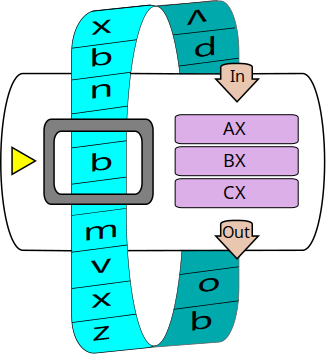
\includegraphics[width=0.5\columnwidth]{figures/methods/squishedCPU_extra.png}
\caption{\textbf{An example virtual CPU from Avida}, with a circular genome (blue), three registers (purple), input and output handlers (tan), and an instruction pointer (yellow) indicating the next instruction to be executed.%
}\label{fig:cpu}
\end{figure}

%=description of Avida organism
An Avida organism is composed of a circular genome of assembly-like computer instructions that are executed in a virtual CPU (Fig~\ref{fig:cpu}). Populations of these organisms are placed in a toroidal world in individual cells where they are allowed to execute, reproduce, compete for space, mutate, and evolve.

%=Avida are self-replicating, but without perfect fidelity
Organisms in Avida are self-replicating, and experience mutation. The genomes of the initial default organisms contain all of the instructions necessary for reproduction. However, the instructions are not copied into an offspring with perfect fidelity. By default, the reproductive copy instruction is faulty, meaning that it will probabilistically introduce errors (mutations) into the offspring genomes. These offspring organisms execute their own genomes even when different from their parent, and in turn pass on their inherited mutations, along with new mutations, to their own offspring (i.e., variation in the systems is heritable).

%=Avida worlds are constrained and thus competition
Avida worlds can be space- or resource-constrained. Avida allows the experimenter to configure many aspects of the environment, thus subjecting the organisms to various kinds of selective pressures.  In many cases, these environments will include resources that can be metabolized by performing specific functions or activities, resulting in a boost to execution speed that gives the organisms a competitive advantage. However, even without explicit external pressures, organisms still experience an implicit pressure to execute more quickly and efficiently. The organisms that run fastest are typically able to also reproduce fastest, and thus out-compete their peers for space.

%=Avida and paper download information
%=[ ] - TODO - populate the new git repos for the dis with data files, etc]
Avida is available for download without cost from \url{http://avida.devosoft.org/}, and specific versions along with data-files to reproduce the experiments described in this thesis may be found at \url{https://github.com/voidptr/avida} and \url{https://github.com/voidptr/dissertation}.


%%%%%%%%%%%%%%%%%%%%%%%%%%%%%%%%%%%%%%%%%%%%%%%%%%%%%%%%%%%%%%%%%%%%%%%%%%%%%%%%%%%%%%%%%%%
%%%%%%%%%%%%%%%%%%%%%%%%%%%%%%%%%%%%%%%%% CHAPTER 2 %%%%%%%%%%%%%%%%%%%%%%%%%%%%%%%%%%%%%%%
%%%%%%%%%%%%%%%%%%%%%%%%%%%%%%%%%%%%%%%%%%%%%%%%%%%%%%%%%%%%%%%%%%%%%%%%%%%%%%%%%%%%%%%%%%%

\chapter{Changing environments promote rapid adaptation in digital organisms}
\label{chap:ce-adaptation}

\section{Background}
The interaction between an environment and possible genomes can be mathematically expressed by a fitness landscape.
%=fitness landscapes are useful math but real-world landscapes are more complex than theory
Fitness landscapes are a mathematical tool to map genetic sequences to reproductive fitness. Many studies have examined the important role that different types of fitness landscapes play on evolutionary dynamics and outcomes, both in biological populations \cite{khan_negative_2011,szendro_quantitative_2013,weinreich_darwinian_2006,nahum_tortoisehare_2015} and in evolutionary computation settings \cite{merz_fitness_2000,humeau_paradiseo-mo:_2013,kallel_theoretical_2013}. However, real-world fitness landscapes are far more complex and varied than the limited or idealized models that are used in most of these studies. Neighboring regions of real landscapes can have starkly different properties from each other based on the effects of and interactions among mutations; as such, a local region of a fitness landscape around a genotype is commonly referred to as its mutational landscape.% (i.e., the mutational landscape).  

%=properties of landscapes depend on architecture
Examples of the type of properties that we are interested in include robustness, epistasis, and modularity, all of which are measurements of how information is organized inside of a genome and commonly categorized as components of an organism's ``genetic architecture''. Isolated pockets in a landscape can often be characteristically different from the landscape as a whole due to the amount and organization of genetic information.  In fact, in most natural fitness landscapes, the vast majority of neighborhoods consist entirely of non-replicating genomes with zero fitness (and thus no genetic information), making life itself appear to be a rare exception \cite{gavrilets_fitness_2004}.

%=evolution is limited to viable areas
Evolution on these convoluted landscapes is clearly limited to those regions that have non-zero fitness, with a selective pressure for fitness to increase. Beyond that, however, populations can evolve toward neighborhoods with specific local properties based on the evolutionary forces acting upon the populations.  For example, high mutation rates drive populations toward neighborhoods with a higher fraction of neutral mutations in an effect dubbed “survival of the flattest” \cite{wilke_evolution_2001}. Similarly, sexual populations tend toward regions of the fitness landscape with more modularity \cite{misevic_sexual_2006} and more negative epistasis \cite{misevic_experiments_2010} than otherwise equivalent asexual populations.

%=understanding dynamics is of broad interest
Understanding these dynamics is of broad interest.  It is important to evolutionary computation, given the strong influence of local landscape properties on the quality of the final solutions that an evolving population is able to obtain. Its relevance to evolutionary biology is equally obvious -- the local landscape that a population occupies will influence the selective forces at play in the population, creating a feedback cycle between these two important evolutionary factors \cite{zaman_coevolution_2014,meyer_repeatability_2012}. Disentangling such interactions is likely to provide further insights into fundamental evolutionary dynamics.  Computational artificial life systems have the advantage of being able to bridge these two realms: they have unconstrained evolutionary dynamics similar to natural systems, while maintaining the ability to rapidly perform experiments and collect any data we need about populations or their local landscapes.
% * <mjwiser@gmail.com> 2016-12-01T20:34:49.014Z:
%
% I can suggest other citations here, so we're not solely citing people out of Charles' and Rich's labs.
%
% ^ <mjwiser@gmail.com> 2017-01-30T18:26:00.719Z:
%
% A few suggested citations here, given Charles' agreement:
% Aita et al 2002.  Surveying a local fitness landscape of a protein with epistatic sites for the study of directed evolution
% Bershtein et al 2006 Robustness–epistasis link shapes the fitness landscape of a randomly drifting protein
% Martin and Lenormand 2006 THE FITNESS EFFECT OF MUTATIONS ACROSS ENVIRONMENTS: A SURVEY IN LIGHT OF FITNESS LANDSCAPE MODELS
% Kvitek and Sherlock 2009 Reciprocal Sign Epistasis between Frequently Experimentally Evolved Adaptive Mutations Causes a Rugged Fitness Landscape
%
% ^ <mjwiser@gmail.com> 2017-01-30T18:26:30.874Z:
%
% I can pick out a few more recent ones if these seem older than you'd prefer.
%
% ^.
% @CAO: Good call Mike!

\subsection{Evolvability and Genetic Architecture}
%=what is evolvability, to us
As described in Chapter~\ref{chap:introduction}, evolvability refers to a series of distinct but overlapping concepts that are generally concerned with adaptation, variation, and/or novelty generation \cite{pigliucci_is_2008}. Depending on your perspective, evolvability can describe the response to selection at the population level\cite{fisher_genetical_1930,houle_comparing_1992}, the ability of populations to adapt to changing conditions\cite{belle_code_2002}, larger phenomena such as variability generation\cite{gunter_p._wagner_perspective:_1996}, 
exploration of neutral spaces and robustness\cite{andreas_wagner_robustness_2005,kitano_biological_2004}, 
generation of novel features\cite{alberch_genes_1991,brookfield_evolution:_2001}, 
or even the potential to generate clade-level innovations\cite{kirschner_evolvability_1998} 
and major transitions\cite{smith_major_1995}. For the purposes this chapter, we will focus on evolvability as the capability of genomes to generate adaptive variation in response to mutation. 

%=how it affects short term evo
In the short-term, this kind of evolvability determines a population's response to selection. This kind of evolvability depends primarily on the organization and interrelation of information in the genome; that is, the genetic architecture, and the resulting genotype-to-phenotype map \cite{gunter_p._wagner_perspective:_1996}. An example of evolvable architecture can be found in some bacterial genomes that contain highly mutable genome regions, called contingency loci. Small sets of insertions or deletions to these regions create transcription frameshifts that alter the expression of nearby coding regions, thus allowing populations to easily switch phenotypes via minor mutations. Contingency loci are most often seen in the genomes of pathogens, which are subject to frequent environmental shifts caused by the host immune system \cite{bayliss_simple_2001}. Thus, these populations are able to produce large amounts of heritable variation despite the reduction in population diversity resulting from population bottlenecks.


\subsubsection{Mutational Landscapes}
%=how mutational landscapes relate
Properties of genetic architectures such as evolvability and robustness are determined by the shape of the resulting mutational landscape (local fitness landscape around a genotype, accessible in a single mutation) \cite{andreas_wagner_robustness_2008}. Robust genetic architectures that can tolerate more mutations without altering their phenotype reside in mutational landscapes that connect to more neutral mutants. Similarly, architectures that more easily switch phenotypes in response to mutation without substantial reduction in fitness, reside in more evolvable regions of genotype-space.

%=not all regions equally accessible
It is worth noting that not all regions of the mutational landscape are equally accessible. Some genome regions may be more resistant to mutation than others \cite{lee_rate_2012}, thereby altering \todo[noinline]{clarify} the probabilities of mutations occurring that lead into certain regions of the mutational landscape. This kind of differential probability may therefore moderate a population's diffusion through the mutational landscape.

% @CAO: How would it be altered?  I'm not sure I understand the last couple of sentences here...
% * <mjwiser@gmail.com> 2017-01-30T18:58:49.934Z:
%
% There are several ways I could interpret this sentence about the Lee paper, so I feel I need to read the paper.  Is it that there are certain regions of a genome that are harder to mutate, either because they are physically constrained or that they are more easily error-checked?  Is it that certain regions of the mutational landscape are more resistant to mutations?  If it's the latter, perhaps a rephrasing along the line of "Some regions of the mutational landscape are more resistant to mutations (preferably with some explanation of how).  As such, regions of the mutational landscape that are bordered by such mutation-resistant regions are less accessible, as the set of genotypes that are mutationally close to them are themselves resistant to mutations."
%
% ^.
% @RCK: Will look into it and clarify.

%=response to selection may be weaker/stronger
Further, response to selection is likely to be weaker in regions of the landscape where there are fewer available mutations that provide potentially adaptive traits, whereas response to selection will be stronger in regions where there are many adaptive variants available within a few mutational steps \cite{alberch_genes_1991,carter_role_2005}. This differential response to selection therefore constrains the ability of populations to diffuse across a fitness landscape.

In order to assess the potential of different regions of the fitness landscape to promote or hinder evolvability, we will use both the \textbf{Genomic Diffusion Rate} ($D_g$)\ref{eq:genomic_diffusion_rate} and the \textbf{Phenotypic Diffusion Rate} ($D_p$)\ref{eq:phenotypic_diffusion_rate}, as normalized across changing environments\ref{eq:expected_fitness_value}.




\section{Methods}

\subsection{Experimental Design}
%=design for experimental environment (CCE vs SCE, and short vs long)
In order to examine the dynamics and mechanisms of evolving populations in changing environments, we performed two sets of experiments. We subjected populations of evolving digital organisms to a set of cyclic changing environments, and a set stochastic changing environments. The cyclic environments were designed to simulate predictable cycles of change, such as day/night or seasonal cycles, whereas the stochastic environments represent less predictable oscillations in environmental states, such as random weather patterns, or climactic changes. These experiments allow organisms to adapt to a predictable set of environments, and explores short-term evolvability dynamics. See Table~\ref{ce-treatments-h}

\missingfigure{A diagram of how the environments are placed. stochastic as jumbled, cyclic as periodic. Harsh is red/blue, Benign is white/blue.}

%=[TABLE - experimental treatments]
\begin{table}[]
\centering
\caption{\textbf{Experimental Treatments}}
\label{ce-treatments-h}
\begin{tabular}{|c|c||c|c|}
\hline
\multirow{2}{*}{ \thead{Treatment} } & \multirow{2}{*}{ \thead{Changing \\ Environment} } & \multicolumn{2}{c|}{ \thead{Rewarded Tasks} } \\\cline{3-4}
& & XOR & EQU \\\hhline{|=|=|=|=|}
Control & \makecell{None \\ (static)} & \makecell{constant \\ $2^3$} & \makecell{constant \\ $2^5$} \\\hline
\makecell{CCE \\ Benign} & Cyclic & \makecell{constant \\ $2^3$} & \makecell{benign \\ fluctuating \\ 0 or $2^5$} \\\hline
\makecell{CCE \\ Harsh} & Cyclic & \makecell{constant \\ $2^3$} & \makecell{harsh \\ fluctuating \\ $-2^5$ or $2^5$} \\\hline
\makecell{SCE \\ Benign} & Stochastic & \makecell{constant \\ $2^3$} & \makecell{benign \\ fluctuating \\ 0 or $2^5$} \\\hline
\makecell{SCE \\ Harsh} & Stochastic & \makecell{constant \\ $2^3$} & \makecell{harsh \\ fluctuating \\ $-2^5$ or $2^5$} \\\hline
\end{tabular} 

\begin{flushleft} Experimental treatments. Four types of changing environment, plus a static control. In the first two treatments, the environment switches in a predictable cycle, whereas in the second two, the environment switches at random intervals. 
\end{flushleft}
\label{ce-treatments}
\end{table}


\subsubsection{Cyclic and Stochastic Changing Environments}
%=explanation of the changing environment treatments - cyclic
For the cyclic environment, we subjected a total of 150 replicate populations of digital organisms to two different treatments of two-phase cyclically changing environments, plus a static control. The environment cycles between 500 updates of reward, and 500 updates of punishment; as such each full cycle is 1,000 updates, or roughly 30 generations. We chose this cycle length after surveying a series of possible values in order to determine an optimal length of time. That is, long enough to allow adaptation to occur and spread through the population, but short enough to reduce the effects of drift destroying vestigial genetic information. For more details about this survey, please refer to Appendix \ref{appendix:ce_sweep}.

In the static control, there is no cycle. Rather, the rewards remain constant. The first phase of the experiment extends for 200 cycles, or 200,000 updates, approximately 6,000 generations.

%=stochastic
The stochastic changing environment experiment is similar to the cyclic environment, except that rather than the environment toggling every 500 updates, the environmental switch happens randomly, with a 0.002 probability of changing on every update. This averages, in the long term, to approximately one switch every 500 updates, but in the short term, the environmental switches are unpredictable.

%=tasks
We set up the system to detect organisms that performed XOR or EQU, two challenging bitwise logical tasks. In the static control, XOR is rewarded with a CPU speed (and thus fitness) multiple of 8, while EQU is rewarded with a CPU speed multiple of 32. In the harsh treatment, as the cycle progresses, the XOR reward remains constant, while the EQU reward cycles between a 32-fold bonus and a correspondingly harsh 32-fold penalty (i.e., CPU speed is divided by 32 when EQU is performed in the off cycle). The benign treatment is nearly identical to the harsh treatment, except that the reward merely goes away in the off-cycle as opposed to incurring a severe penalty.

%=differences between tasks
In both environments, we identify EQU as the \textit{Fluctuating Task}. XOR, because it is rewarded continuously, is the \textit{Backbone Task}, and is used as a background for comparing the separation or intertwining of functional genetic components in the evolution of EQU. Further, the 4-fold difference in reward level between XOR and EQU encourages the evolution and maintenance of EQU when possible.

%=the organisms are ...
For all of the experiments described in this section, we held the individual genomes at a fixed length of 121\footnote{As part of our initial controls, we hand-wrote an organism with separated sections that performed XOR and EQU. This hand-written organism had 121 instructions and as such we used this genome length as a constraint for the evolve organisms as well.} instructions, but tested the new genomes for mutations after each successful replication event at a substitution probability of 0.00075 per site. We configured the Avida world to have local interactions on a toroidal grid that is 60-by-60 cells (3600 cells in total), and we seeded the initial populations with an ancestor that was previously evolved to perform XOR and EQU under a static reward. The genetic architecture for performing XOR and EQU is tightly intertwined in this ancestral organism, as it was evolved with no selective pressure for modularity.


\section{Results and Discussion}
%=summary - we found that CE evolved populations are genetically distinct. Stochastic pretty similar to CCE
Our experiments demonstrate that digital organisms that were evolved in changing environments differ substantially from those that evolved in static environments in a number of ways. These differences include the number of mutations that fix in the lineage from the ancestor (the ``phylogenetic depth"), key metrics of their genetic architecture, and the presence of reservoirs of pseudogenes that change the nearby mutational landscape. These features represent adaptation to the larger regime of repeated environmental switching. We also show that while populations evolved in cyclic environments are slightly better adapted to change than those that evolved in stochastic environments, in most measures of adaptation and short-term evolvability, these differences are generally not significant. This result indicates that while regular periodicity may offer a slight advantage for adaptation, stochastic environments perform similarly in most respects. 
\todo[noinline]{look for un-anchored "this"s}

\subsection{Cyclic Changing Environments}
We will begin by examining the characteristics of populations evolved in cyclic changing environments.

\subsubsection{Evolutionary History and Population Structure}
%=more phylogenetic depth
Evolution in the harsh cyclic changing environment resulted in many more mutations fixing, and thus populations with substantially higher phylogenetic depth as compared to those evolved in static or benign environments. At each environmental shift, adaptive mutations rapidly swept and fixed in the populations. (Fig~\ref{fig:flamegraph})

%=[FIGURE - flamegraph]
\begin{figure}[!h]
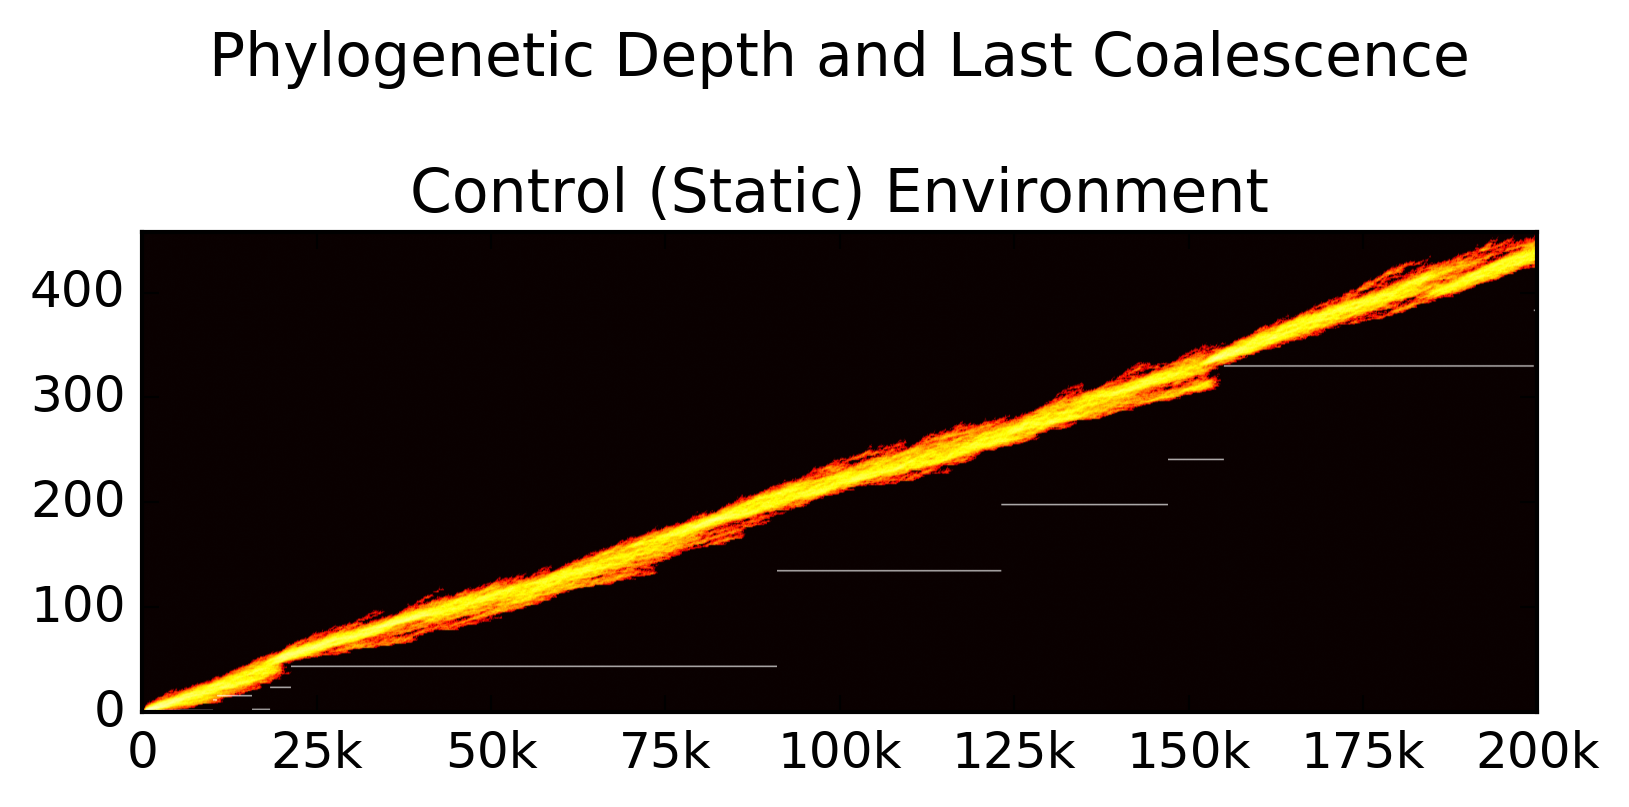
\includegraphics[trim={-0.88cm 0 0.25cm 0},clip,width=0.65\columnwidth]{figures/CE/control__phylodepth_with_coalescense.png}
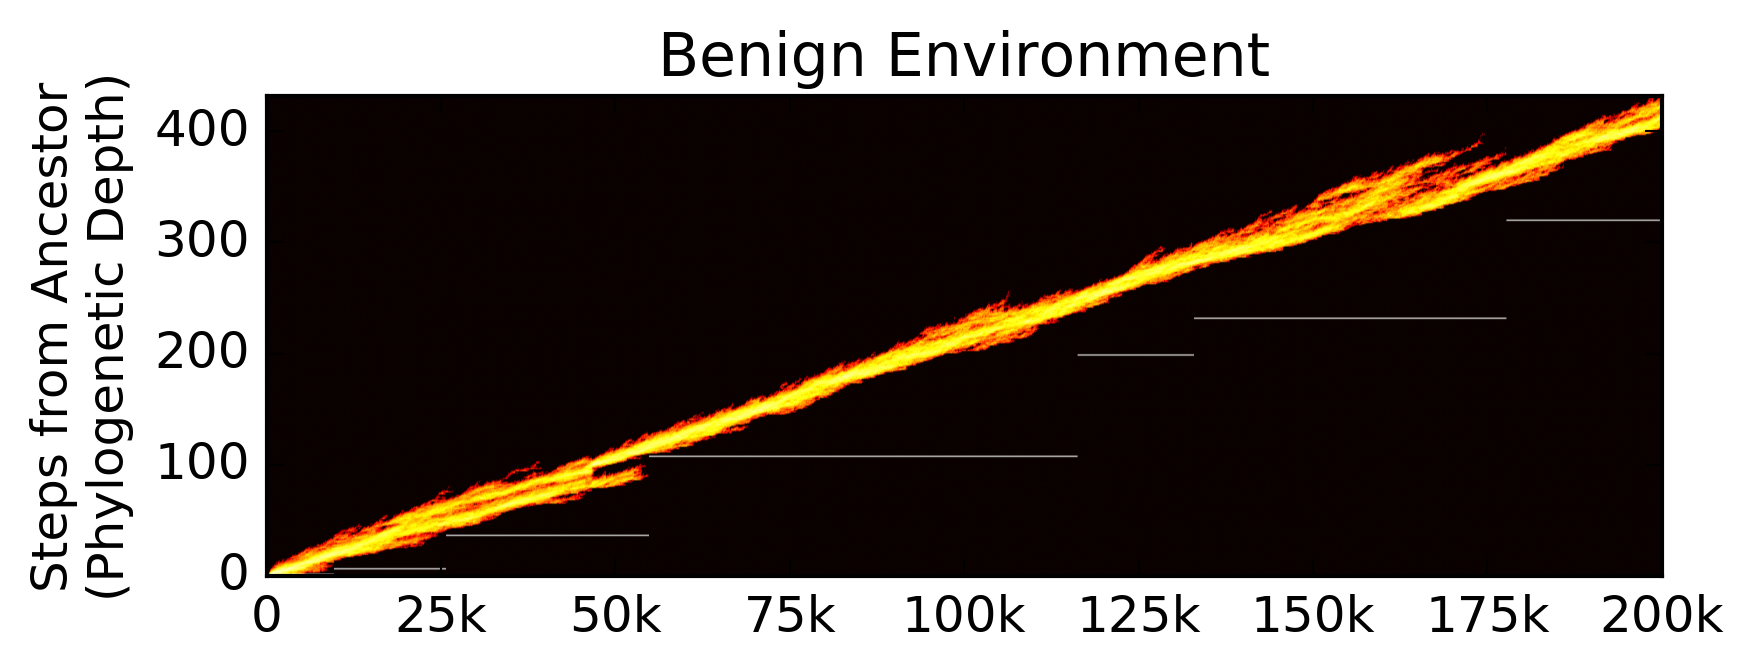
\includegraphics[trim={0.2cm 0 0.25cm 0},clip,width=0.65\columnwidth]{figures/CE/benign__phylodepth_with_coalescense.png}
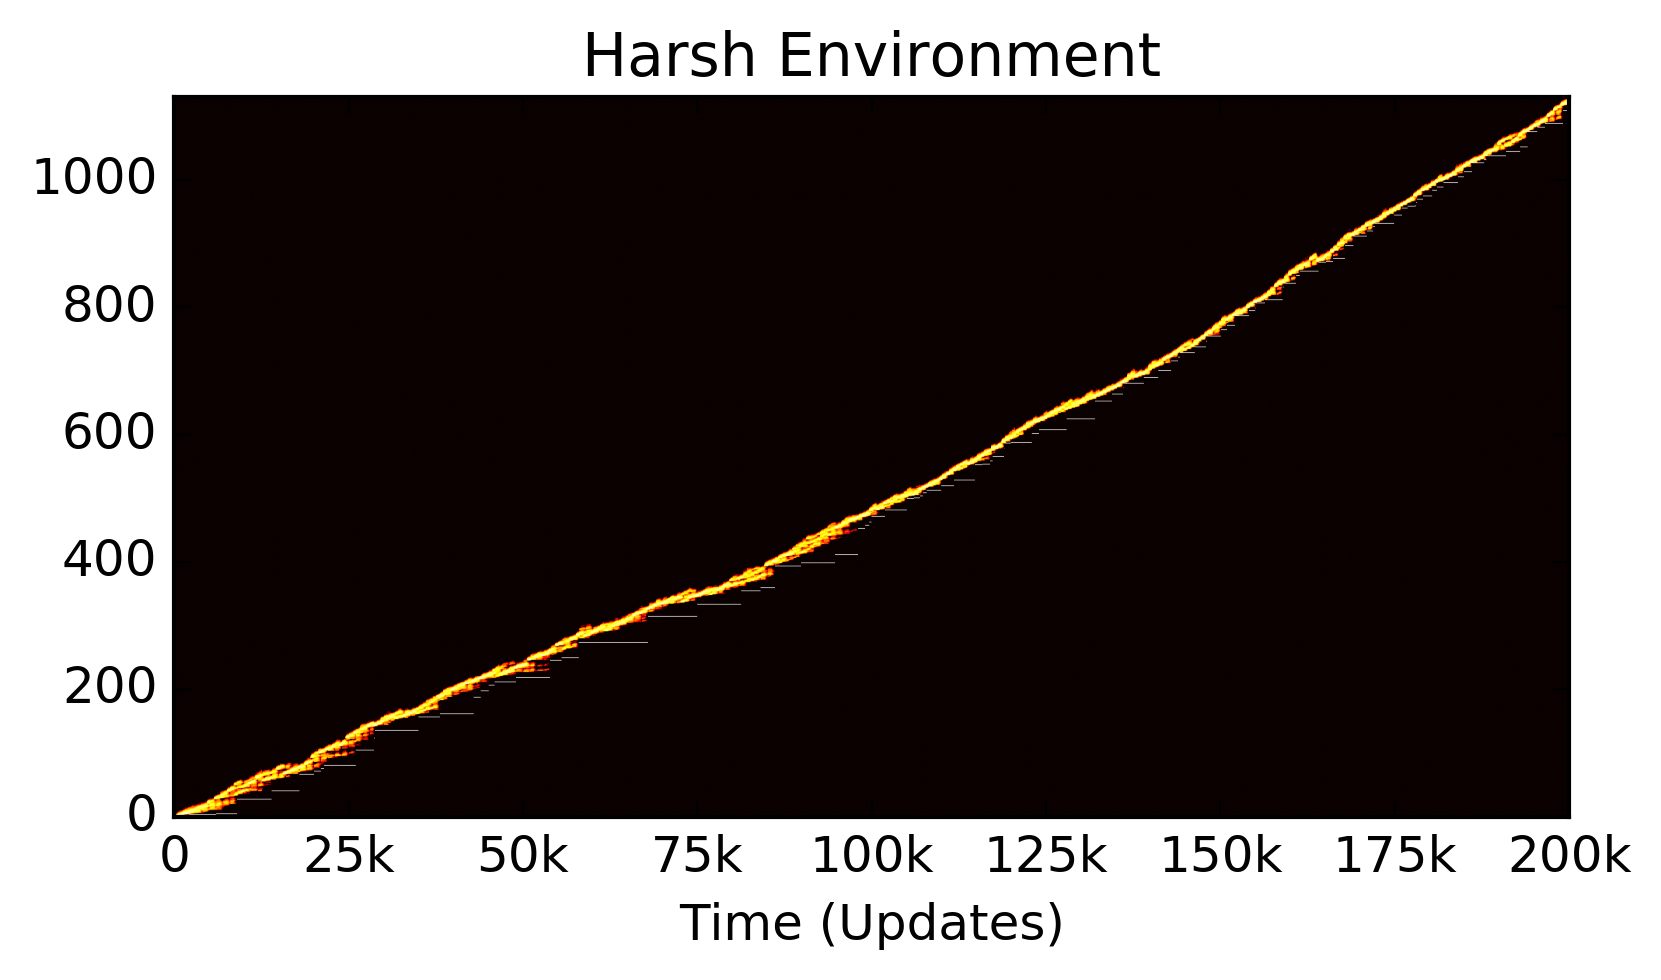
\includegraphics[trim={-0.63cm 0 0.25cm 0},clip,width=0.65\columnwidth]{figures/CE/harsh__phylodepth_with_coalescense.png}
\caption{\textbf{Phylogenetic depth over time} of a sample population evolved in each of the three treatments of the cyclic changing environments. White horizontal lines mark the depth of the most recent common ancestor, and discontinuities in this line indicate that the most recent common ancestor has changed, and thus that a sweep occurred, or that a competing clade went extinct. The control treatments had a mean of 18 sweeps (STD=9.05), the benign treatments had a mean of 21 (STD=19.05), and the harsh treatments had a mean of 88 sweeps (STD=23.37). Note the difference in scales between y-axes: the control-evolved population has a maximum depth of 400 mutational steps from ancestor, while the harsh-evolved has upward of 1100. %
}\label{fig:flamegraph}
\end{figure}

%=more genetic diversity
The populations that evolved in the control and benign environments displayed more genetic diversity as compared to those evolved in the harsh cyclic environment, which underwent a bottleneck at each cycle shift. Because a selective sweep reduces current diversity within a population, the smaller number of sweeps
% @CAO it looks like it wasn't just a smaller number of sweeps, but that the sweeps took MUCH longer to occur, to the point where it's hard to even dub them sweeps at all...  more fixation events?  Mike should weigh in here too.
in the benign and control treatments led populations in them to have higher standing diversity for most of their evolutionary history than those populations from the harsh changing environment.  Despite this higher standing diversity in the benign and control treatments, regions of low diversity are still evident in the genomes of these populations, implying purifying selection on the traits encoded at these sites (see Fig~\ref{fig:entropy}).
% * <mjwiser@gmail.com> 2017-01-30T19:39:00.542Z:
%
% I feel like this figure would be easier to talk about if you split it into three panels, and mention that each panel has both an upper and a lower part.  It would also probably be easier to read if the axes on the left were on the top panel, rather than the middle one; since you have two graphs in each panel, it doesn't make sense to just have a single axis label off to the side.  However, you probably *can* have only a single x axis label, since the axes are the same for all the panels, and for both graphs within a panel.
%
% ^.

\todo[inline]{fix figure below so that it's two separate figures. Separate the mean entropy to its own figure.}
	\begin{figure}[!h]
	%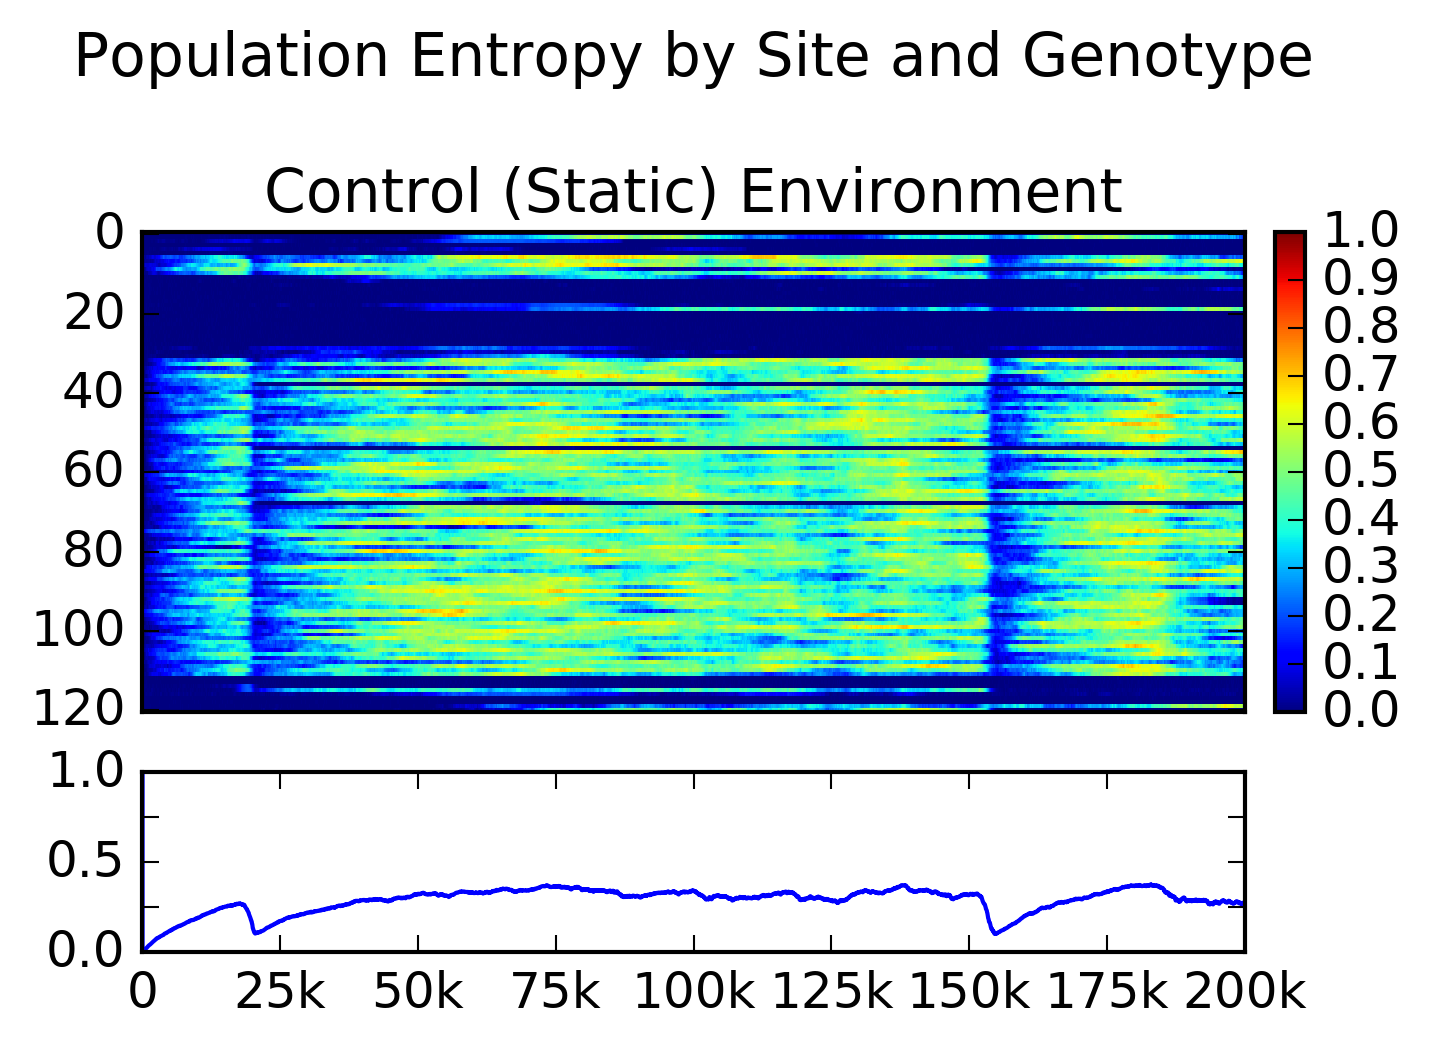
\includegraphics{figures/CE/control__entropy}
	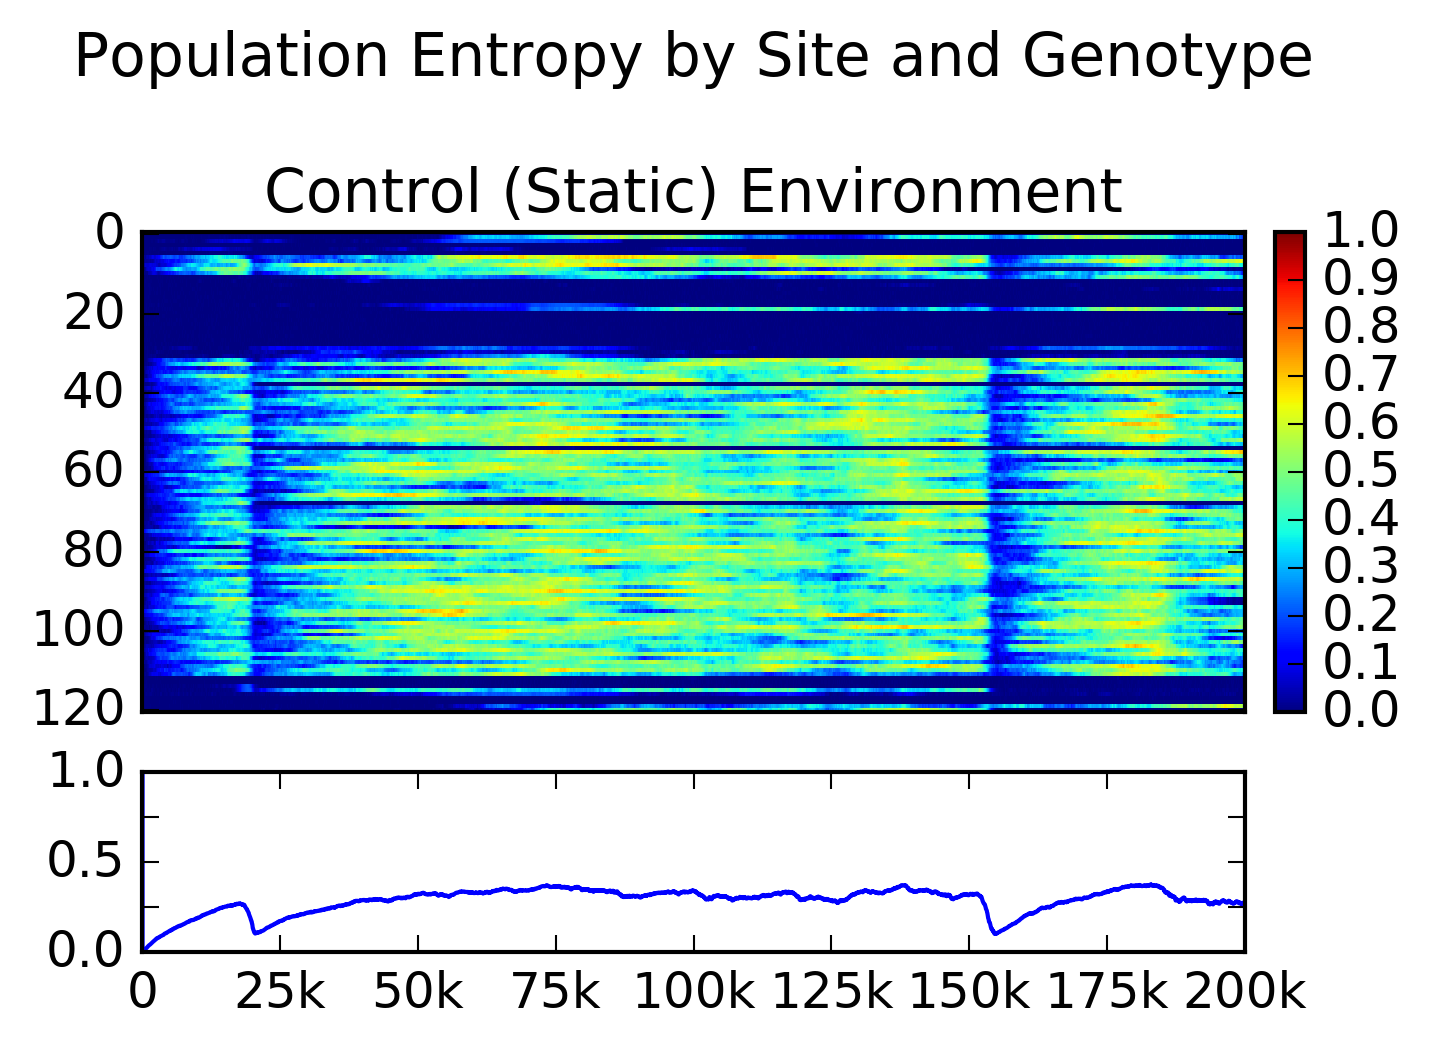
\includegraphics[trim={-0.85cm 0 0.1cm 0.2cm},clip,width=0.5\columnwidth]{figures/CE/control__entropy}
	%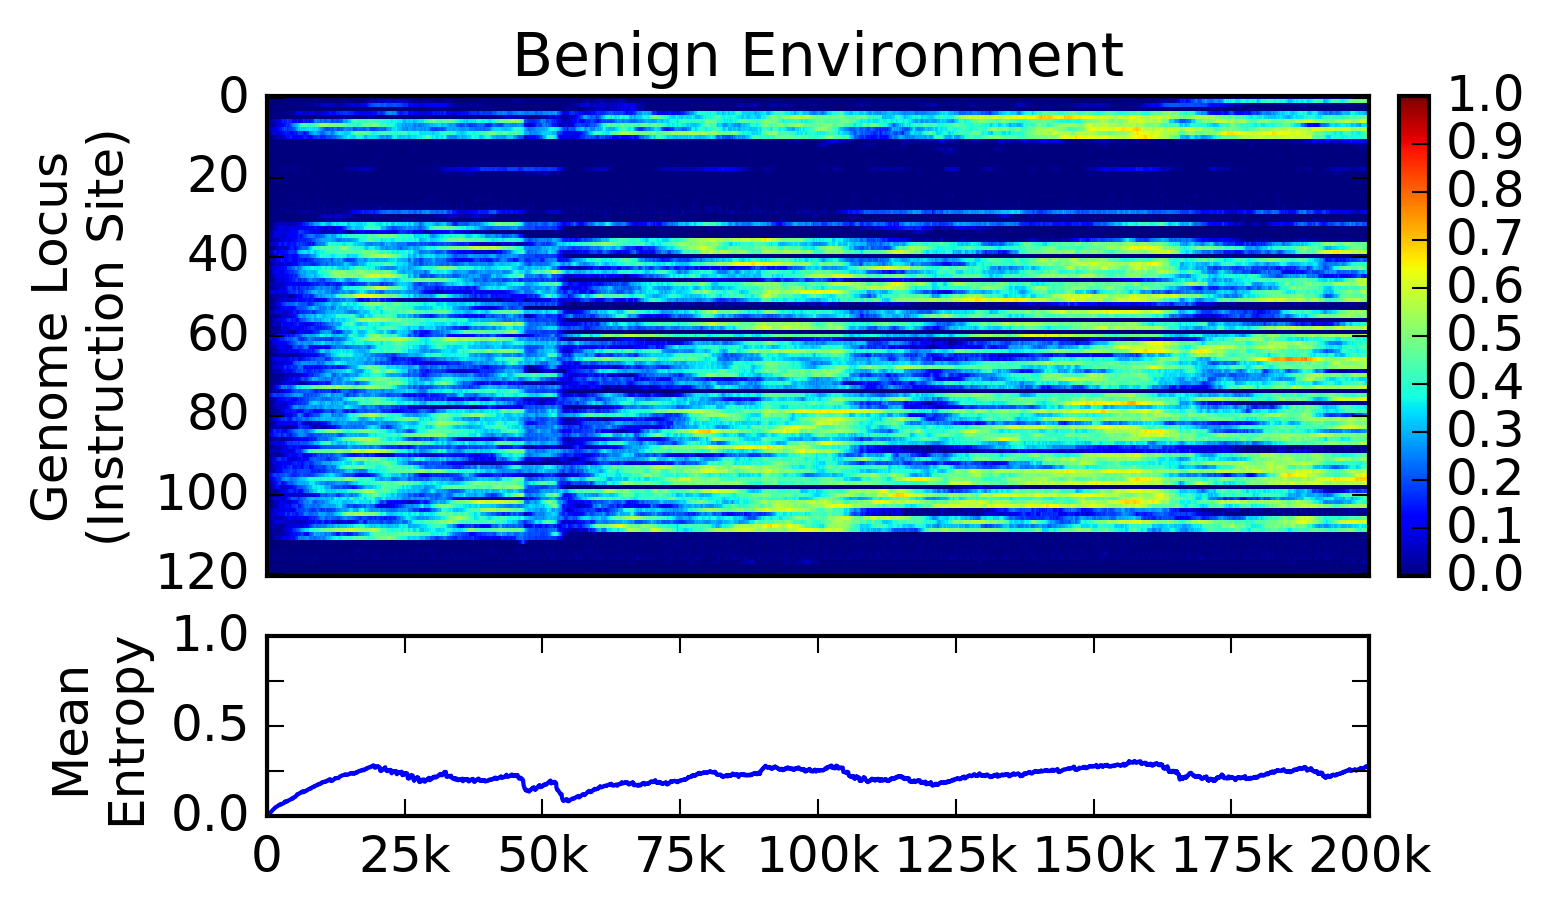
\includegraphics{figures/CE/benign__entropy}
	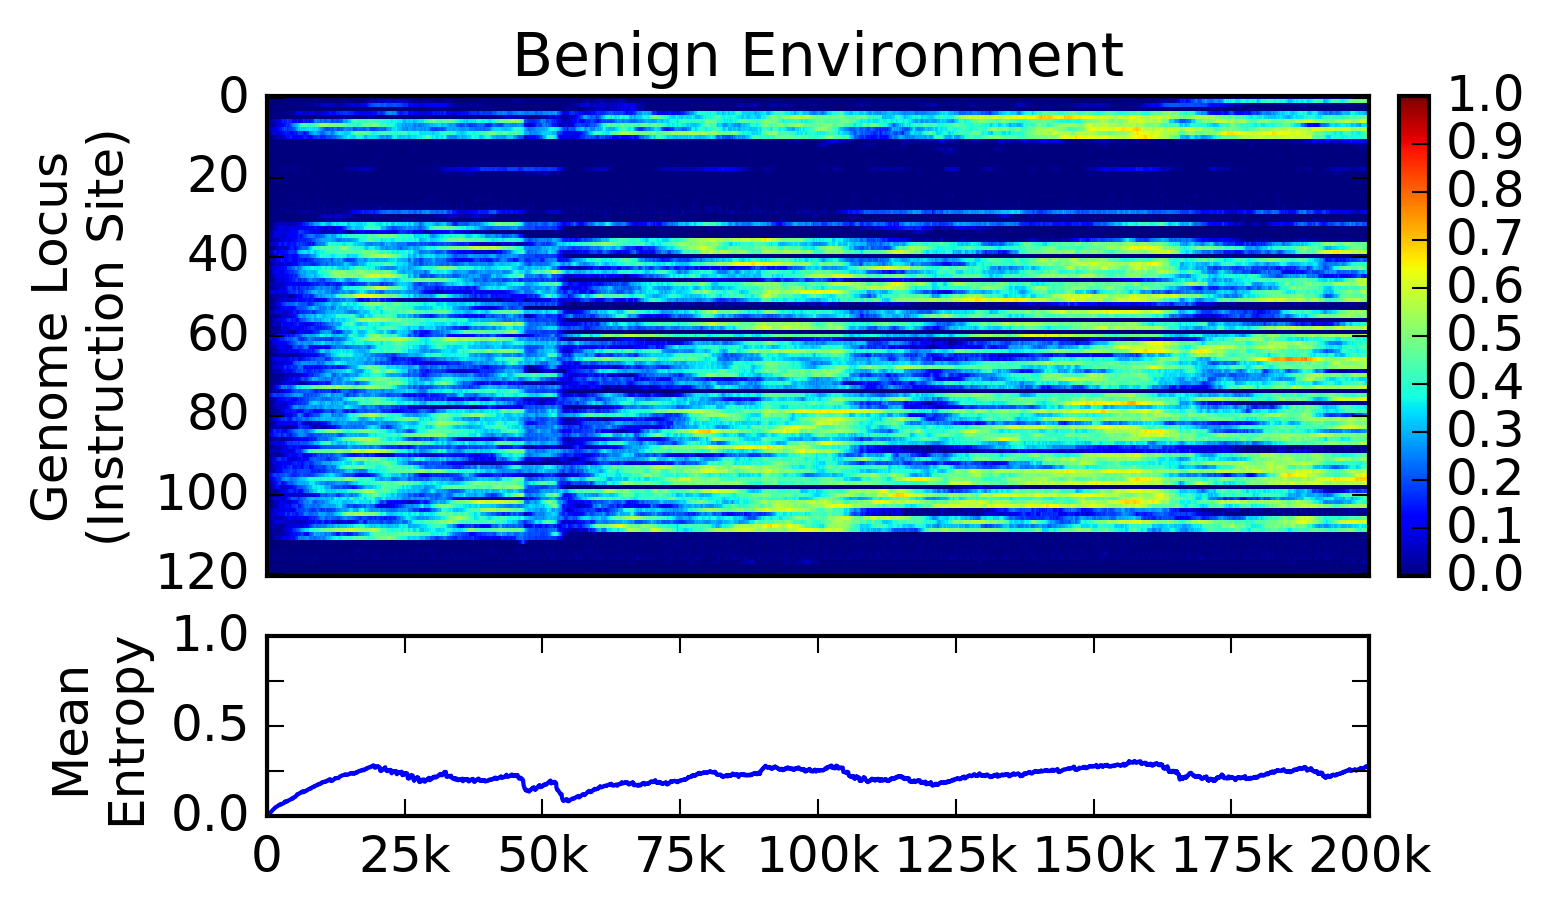
\includegraphics[trim={0.25cm 0 0.1cm 0},clip,width=0.5\columnwidth]{figures/CE/benign__entropy}
	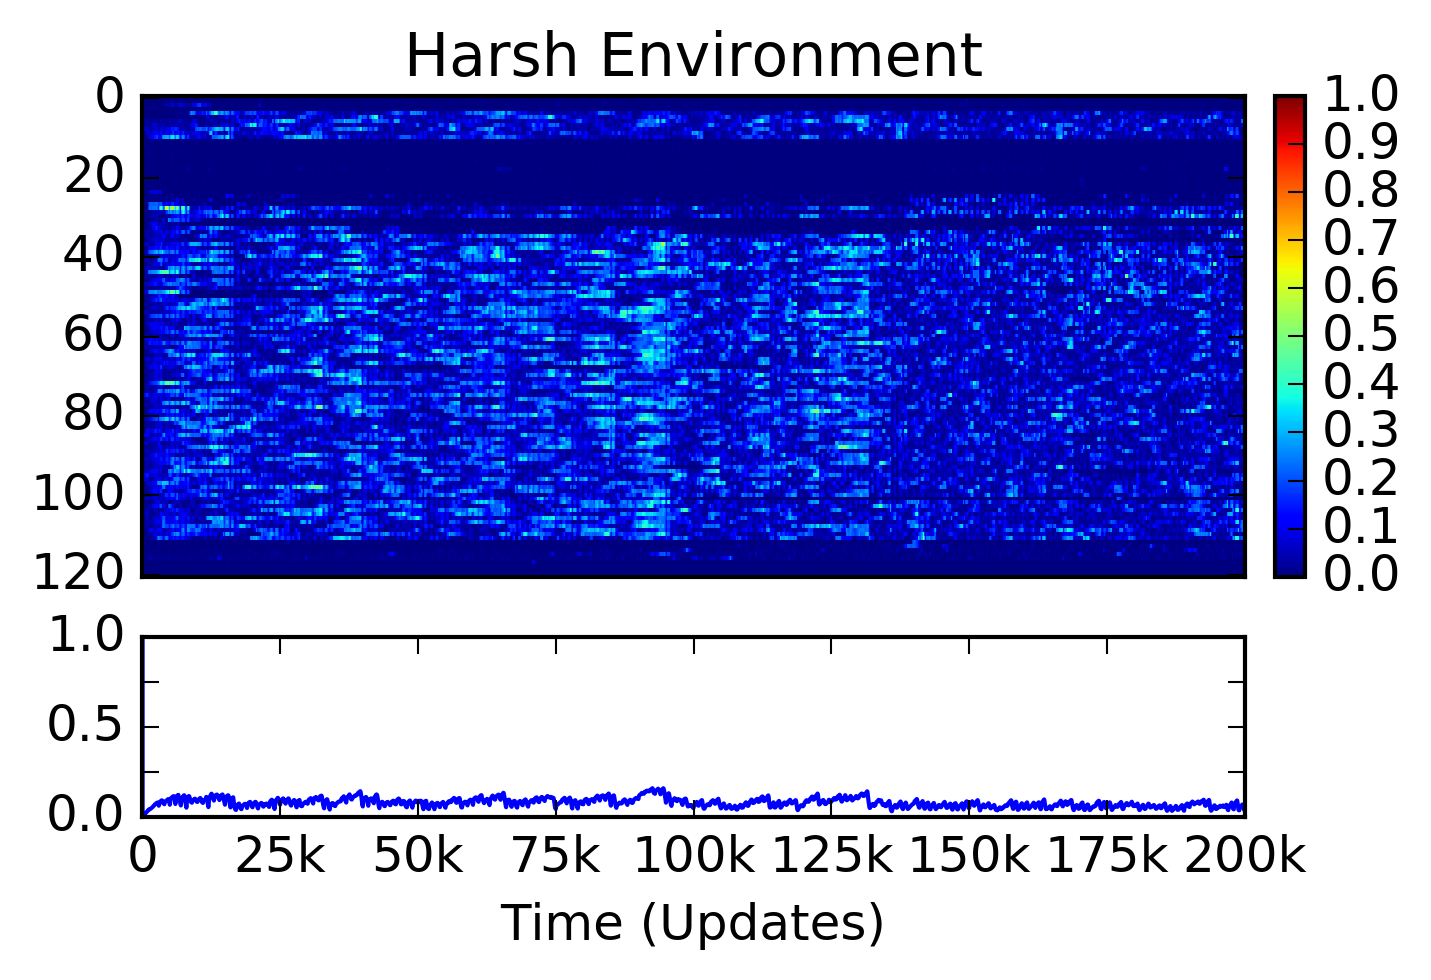
\includegraphics[trim={-0.85cm 0 0.1cm 0},clip,width=0.5\columnwidth]{figures/CE/harsh__entropy}
	\caption{\textbf{Population Per-site Entropy over time} of a representative sample population. Each vertical slice represents the per-site entropy of the population at each update, both by genetic locus (upper), and overall population mean (lower). Hotter colors (red/orange/yellow) indicate greater diversity at this locus, while cooler colors (blues) indicate the a locus is more consistent across the population. Mean population entropy indicates the relative diversity of the population at any given time, while the per-site entropy shows where in the genomes the population diversity is located.   %@CAO: I'm agreeing with Mike that we might want to make this two graphs.  I added a bit in the description about the cooler colors just to lead the reader by the hand as much as possible.
	}\label{fig:entropy}
	\end{figure}


\subsubsection{Genetic Architecture}
%=genetic architecture is different in benign and harsh vs control
\todo{clarify wording}
The selective shifts in both benign and harsh changing environments result in qualitatively different architectural styles from the static control environment. The task arrangements evolved under both experimental treatments are much more scattered throughout the genome than in the control. Specifically, the bulk of the sites responsible for performing the fluctuating task (EQU) did not overlap with the backbone task (XOR), except for a core region, which represents portions of the tasks that are shared between XOR and EQU. (Fig~\ref{fig:lineage})
% @CAO: I'm not positive I understand this description for how things are laid out.  It might be worth putting a bit more detail here, and highlighting also that there is a lot more separation in the harsh environment (or so it seems).  Should we talk more here about why all of this is the case (highlighting that we are speculating) or will that come later?

\todo{polish this figure, task layout, make three separate figures}
	\begin{figure}[!h]
	\setlength{\fboxsep}{0pt}%
	\setlength{\fboxrule}{0pt}%
	\fbox{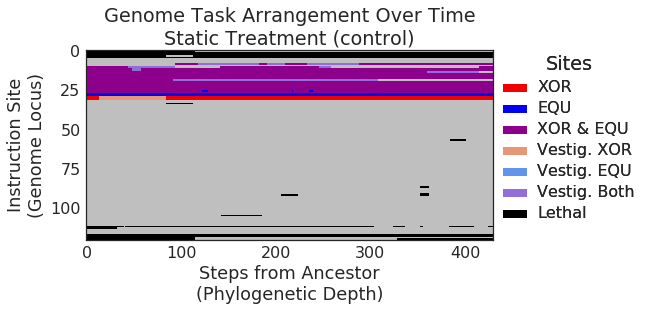
\includegraphics[width=0.5625\columnwidth,trim={-0.82cm 0 5.5cm 0.25cm},clip]{figures/CE/control__whole_taskmap.png}}\fbox{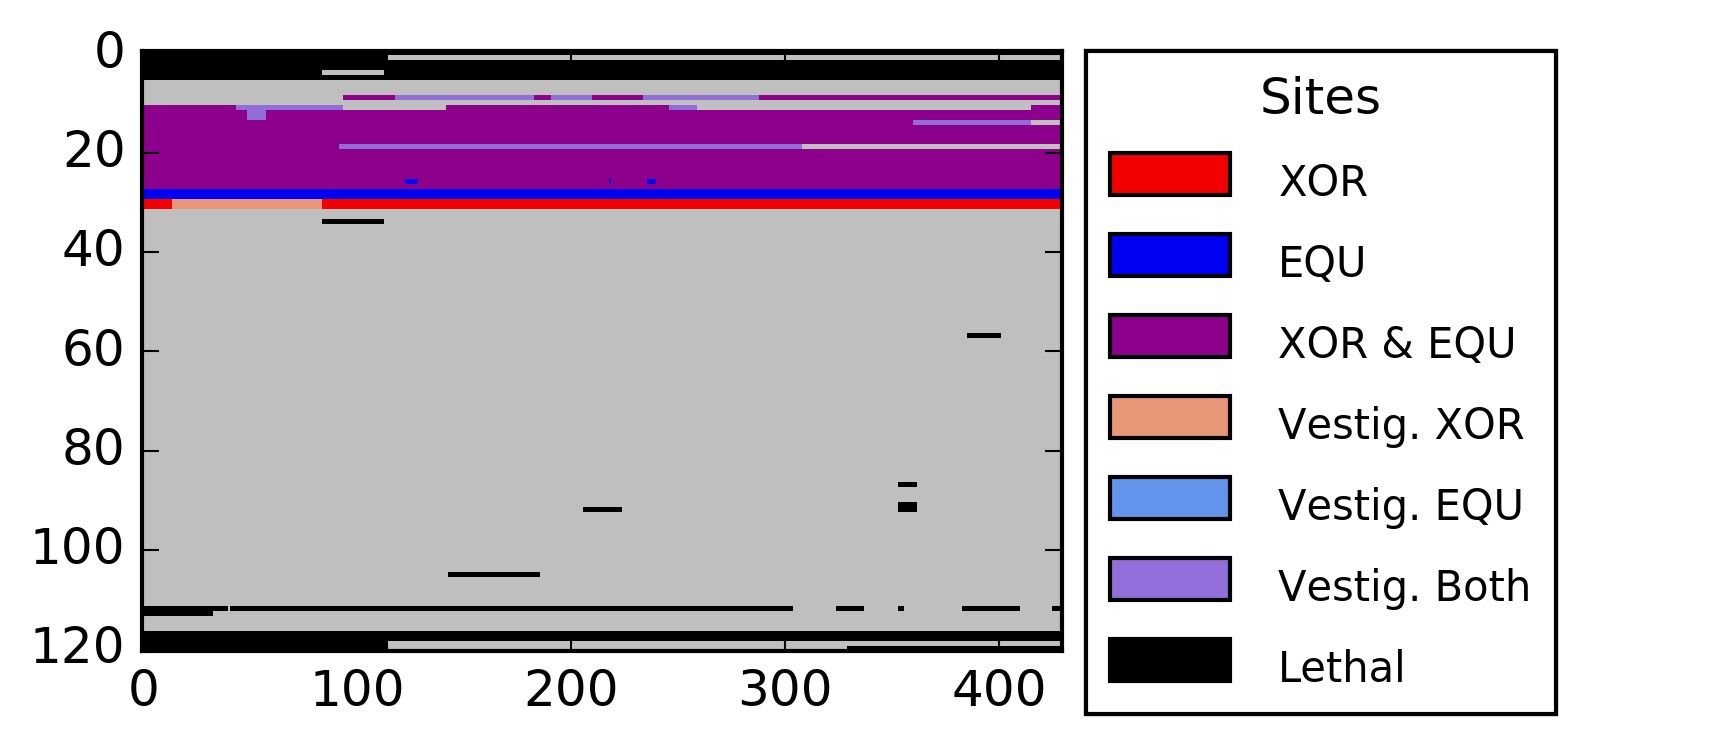
\includegraphics[width=0.1875\columnwidth,trim={9.1cm 0.15cm 1.3cm 0},clip]{figures/CE/legend__whole_taskmap.png}}
	\fbox{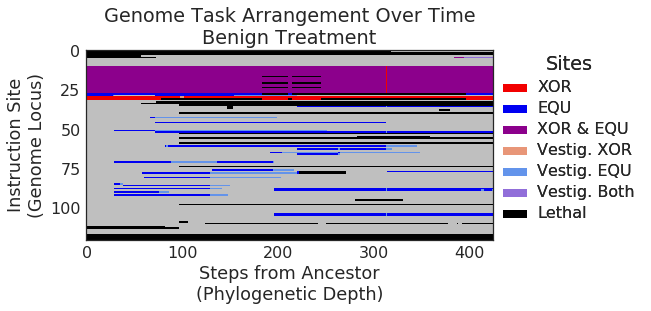
\includegraphics[width=0.75\columnwidth,trim={0.2cm 0 2.3cm 0},clip]{figures/CE/benign__whole_taskmap.png}}
	\fbox{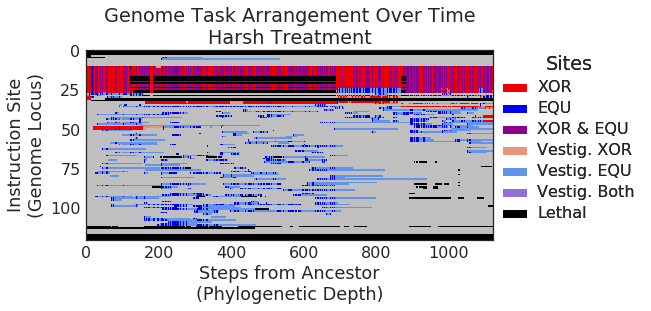
\includegraphics[width=0.5\columnwidth,trim={-0.82cm 0 5.2cm 0},clip]{figures/CE/harsh__whole_taskmap.png}}
	\caption{\textbf{Varying genetic architecture of XOR and EQU over time} for the final dominant genotype in a randomly selected replicate. Proceeding from the left of each figure, each vertical slice represents an organism along the line-of-descent to the final dominant.
	Positions along the Y-axis represent each genome locus; loci in an organism are colored based on the tasks that they code for. Sites in \textbf{red} are active sites that code for the XOR task only, sites in \textbf{blue} are active sites for the EQU task only, and \textbf{purple} sites code for both XOR and EQU. Knockouts to the sites in black are lethal to the organism. Sites in the lighter colors (tan, light blue, lavender) represent vestigial sites for XOR only, EQU only, or both tasks, respectively. As we proceed from left to right, we can see the evolutionary history of the final dominant genotype.}
	\label{fig:lineage}
	\end{figure}

%=arch of control, scattered XOR
In contrast, the architecture of XOR and EQU remain tightly intertwined in the control, and site positions do not change substantially over the course of the experiment. In the benign treatment, many more regions that perform the fluctuating task (XOR) are scattered throughout the genome, but site positions remain relatively fixed throughout the run after an initial adaptive phase. In the harsh treatment, not only are the active sites scattered, but the positions of active sites change and proliferate wildly over time.

%=reservoir of vestigial sites
Interestingly, populations evolved in both the benign and harsh treatments also show development of a large reservoir of formerly functional, now vestigial, sites; that is, sites that remain unchanged from when they were previously active in performing a task, but were disabled by a mutation elsewhere and are thus now neutral. These vestigial pseudogene-like sites appear to be important for allowing the organisms to quickly re-adapt as the fluctuations in the environment restore the previously-rewarded functions. (Fig~\ref{fig:CCE_func_vestigial})

%=[FIGURE - functional vs vestigial sites]
%\todo[color=green]{stats for figure}
	\begin{figure}[!h]
	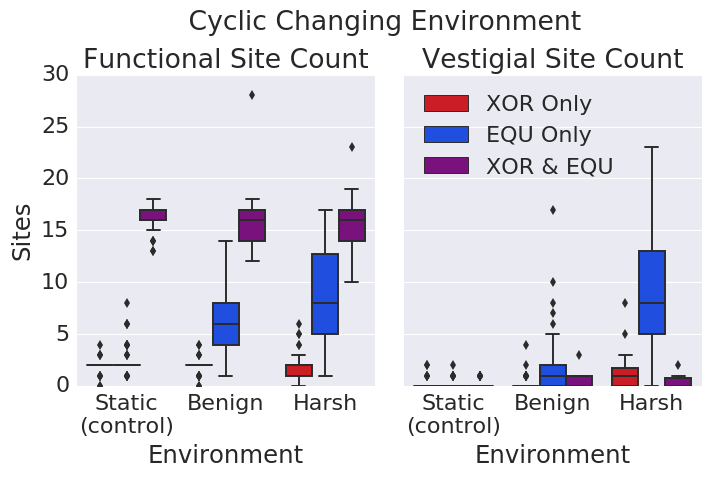
\includegraphics[trim={0 0 0 0}, clip, width=0.75\columnwidth]{figures/CE/CCE_func_vest__box.png}
	%% TODO - generate the stats
	\caption{\textbf{Number of functional and vestigial sites by treatment}. The harsh environment has a significantly larger number of vestigial sites for the fluctuating (EQU) task compared to the benign treatment or control (Wilcoxon Rank-Sum Z = -6.57 and -8.33, p $<<$ 0.0001).
%	\todo[inline]{stats}
	%\todo{stats}%
	%old --- (One-Way ANOVA F(2,132) = 54.35, p $<<$ 0.0001).
	% @CAO: Just a reminder to do the stats!
	}
	\label{fig:CCE_func_vestigial} %% FIGURE 5
	\end{figure}

\subsubsection{Nearby mutational landscape}
\todo[inline]{add figure of the nearby landscape showing how mutations relate 1 and 2 steps out., a couple of nice figures showing both changes in detrimental mutations and phenotypic distribution.}

%=one-step survey of the mutational landscape 
\todo{fix wording to clarify}
In order to identify the role that these pseudogene-like structures play, we performed a survey of the single-step mutational landscape surrounding the most abundant genotype at the end of the experiment for each replicate population. This landscape contained 3,025 distinct mutants (121 loci with 25 possible mutations per locus) in each of the 50 replicates per treatment, for a total of nearly 450,000 mutants surveyed. We found that the availability of reservoirs of vestigial sites shifted the change-evolved organisms' position in the mutational neighborhood, such that a task that was lost due to mutation remains more accessible via one or two additional mutational steps, beyond the single-step reversion mutation. (Fig~\ref{fig:CCE_single_step}, ~\ref{fig:CCE_two_step})
% @CAO: This last part doesn't make a lot of sense -- CLEARLY if a single mutation causes a task loss, the corresponding reverse mutation would cause that task to be regained.  As such, do you mean that there a MORE paths back to the task in the changing-environment treatments as compared to the static control?
% @RCK: Yes, that's what this means. "More often, above". I can clarify. -- TODO
\todo[inline]{Todo, clarify per Charles's comment above}

%=[FIGURE - Frac 1-step]
%\todo[color=green]{stats for figure}
	\begin{figure}[!h] %% FIGURE 6
	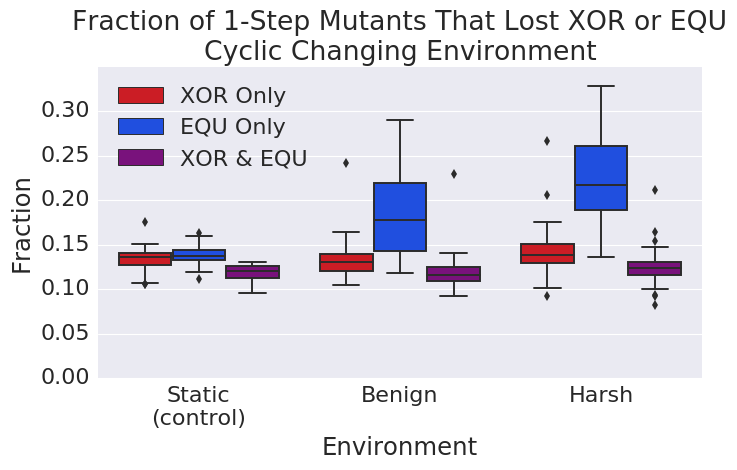
\includegraphics[trim={0.2cm 0 0 0.2cm},clip,width=0.75\columnwidth]{figures/CE/CCE_frac_1step__box.png}
	%% TODO - stats
	\caption{\textbf{A survey of the single-step mutational neighborhood} around organisms that performed the fluctuating task. Note that in both the benign and harsh treatments, there were significantly more mutants that lost the EQU task as compared to the control (Wilcoxon Rank Sum Test: Z = -5.46 and -7.80 respectively, p $<<$ 0.0001). This result indicates that it was easier for the organisms in both treatments to turn off the EQU task in response to one mutation. 
	%\todo[noinline]{TODO STATS}%
	% old -- (Wilcoxon Rank Sum Test: Z = -6.59 and -6.70 respectively, p $<<$ 0.0001)
	}\label{fig:CCE_single_step}

	\end{figure}
%=[FIGURE - Frac 2-step]
\todo[color=green]{stats for figure}
%@CAO - I wonder if it would be interesting to list the number of ways that this happened to be clear that we're not just talking about undoing the changes that caused the loss in the first place.
\todo{Add to caption per Charles's comment above}
	\begin{figure}[!h] %% FIGURE 7
	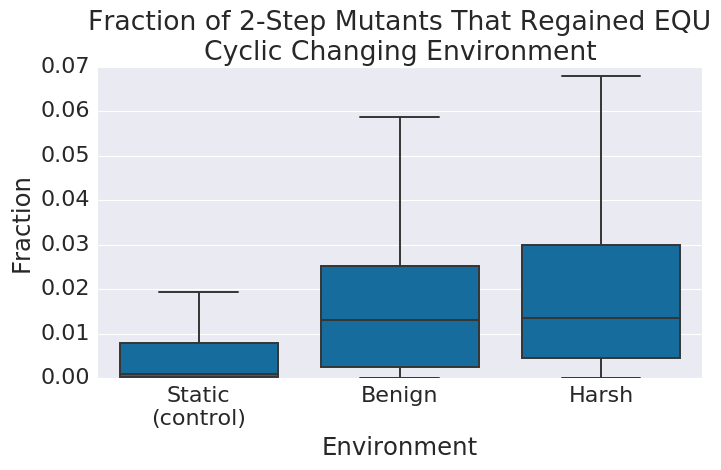
\includegraphics[trim={0.2cm 0 0.4cm 0.25cm},clip,width=0.75\columnwidth]{figures/CE/CCE_frac_2step__box.png}
	%TODO - stats

	\caption{\textbf{A survey of the two-step mutational neighborhood} of the organisms that lost EQU function in the one-step survey. We found that in both the harsh and benign treatments, there were significantly more organisms that regained function in response to mutation than the control. (Wilcoxon Rank Sum Test: Z = -47.9 and -57.82 respectively, p $<<$ 0.0001). This result indicates that it was easier for the organisms in both fluctuating environments to regain the task in response to one additional mutation, beyond a single reversion. 
	%\todo[noinline]{TODO STATS}
	%(Wilcoxon Rank Sum Test: Z = -6.11 and -7.38 respectively, p $<<$ 0.0001)
	}\label{fig:CCE_two_step}
	\end{figure}

%=measured D_g, D_p, found similarity in D_g, increase in D_p 
We also measured the proportion of non-deleterious mutants in the nearby fitness landscape. We found that between all treatments, this proportion
remained approximately the same. However, we found that the proportion of these mutants with different (potentially adaptive) phenotypes increased in the changing environments. In this way, the organisms from the changing environment treatments have an advantage over organisms from the control runs in terms of the short-term evolvability of the fluctuating task. This result indicates real adaptation, not only to resources in their local environment, but a direct adaptation to the environmental change. (Fig~\ref{fig:CCE_diffusion_rate})
\todo[color=green]{add stats for this paragraph}

\todo[inline, color=magenta]{TODO - add paragraph describing/speculating about why Benign loses EQU almost as well as Harsh}
% @CAO: I also get why we should expect to see EQU lost easily in the Harsh changing environment, but why is it also lost so easily in the benign environment.  Should we speculate here?  (Or do you below?)  More generally, why do you think this is the case?
% @CAO: One other thought for how this result may happen.  Maybe in the control there is a pressure for EQU to evolve to be more robust, whereas the changing environment just doesn't give it time to evolve robustness.  I can't think of a way to easily disentangle those explanations though...
% @RCK: clarify that benign are lost due to drift.
% @RCK - NOTE TO SELF -- see about joining vestigial sites paper with Matt's bias work. Are vestigial sites useful because they are random building blocks available (equivalent to mutational bias), or is there a deeper functional structure. Does order matter?

%=[FIGURE D_g D_p]
\todo[color=green]{stats}
	\begin{figure}[!h] %% FIGURE 8
	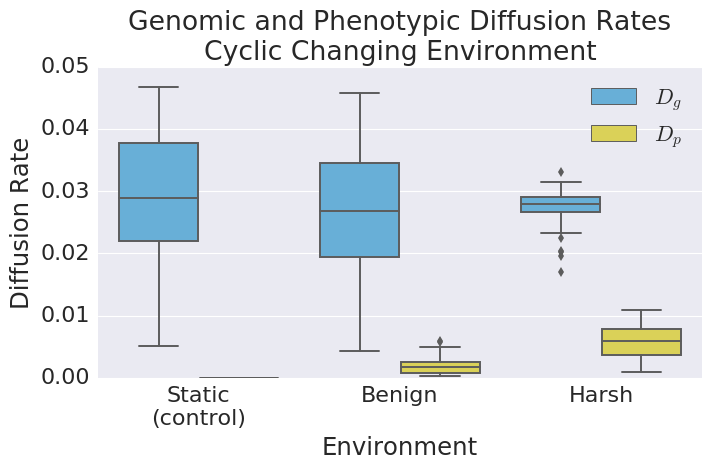
\includegraphics[trim={0.2cm 0 0.4cm 0.25cm},clip,width=0.75\columnwidth]{figures/CE/CCE_D_g_D_p__box.png}
	\caption{\textbf{Genomic and Phenotypic Diffusion Rates}, showing the probabilities of producing offspring that are genotypically ($D_g$) or phenotypically ($D_p$) distinct from the parent, while not reducing fitness.
	Note that while overall neutral exploration capacity remains relatively stable between treatments (Kruskal Wallis: H(2) = 1.4, p = 0.48), phenotypic exploration capacity is increased in both treatments, but especially in the Harsh treatment. (Wilcoxon Rank-Sum Test: Z = -7.42 and -7.77 respectively, p $<<$ 0.0001). This result indicates that changing environments promote the phenotypic evolvability of populations in particular.
	}\label{fig:CCE_diffusion_rate}
	\end{figure}




\subsection{Stochastic Changing Environments}
%= contrary to expectations, SCE weren't better at evolvability (D_g/p)
Contrary to our expectations, stochastic changing environments were, overall, no more effective at
%@CAO - Just "no more" effective, not less?
%@RCK - It was a mixed bag. I don't feel confident enough to definitively say less.
promoting evolvability than cyclically changing environments. Harsh environments performed slightly worse, whereas benign environments were slightly better, though neither result was consistently statistically significant. There was a slight but significant reduction in the Phenotypic Diffusion Rate ($D_p$) between the cyclic and stochastic harsh changing environments; $D_p$ settled on a lower median (Mdn = 0.0) in the stochastic harsh treatment as compared to the cyclic harsh (Mdn = 0.0058) (Wilcoxon Rank-Sum Test: Z = -6.19, p $<<$ 0.0001), indicating a lower probability of the population producing offspring that would switch phenotypes neutrally. In the Benign treatments, however, Stochastic environments fared slightly better than cyclic, though this result was only barely statistically significant (Wilcoxon Rank-Sum Test: Z = 2.2, p < 0.03). (Fig~\ref{fig:CSE_diffusion_rate}) 

%=[FIGURE - D_g/p]
	\begin{figure}[!h] %% FIGURE 12
	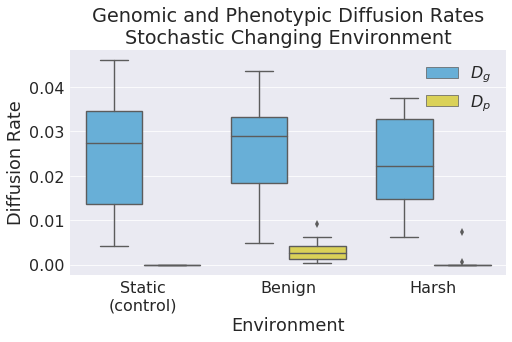
\includegraphics[trim={0.2cm 0 0.4cm 0.25cm},clip,width=0.75\columnwidth]{figures/CE/CSE_D_g_D_p__box.png}
	\caption{\textbf{Genomic and Phenotypic Diffusion Rates} in stochastic changing environments, showing the probabilities of producing offspring that are genotypically and phenotypically different from the parent, while remaining fitness neutral or better. As in the cyclic environment, $D_g$ remains stable for the Benign treatment, but drops slightly in the Harsh as compared to the control, though this drop isn't statistically significant (Kruskal Wallis H(2) = 1.11, p = 0.57). Harsh $D_p$ however, is significantly lower than seen in the cyclic environment treatment (Wilcoxon Rank-Sum Test: Z = -6.19, p $<<$ 0.0001). This result shows that harsh stochastic environments may not be as effective as cyclic environments at increasing the probability that organisms will produce phenotypically different, yet neutral offspring.
	}\label{fig:CSE_diffusion_rate}
	\end{figure}

%=1 and 2-step, slightly reduced
Despite the reduced $D_p$ in the harsh treatment, both the overall fraction of 1-step mutants that lost EQU, and the fraction of 2nd-step regaining of EQU, were only very slightly reduced in comparison to the cyclic treatments, and this effect was not statistically significant. This result indicates that stochastic harsh environments are certainly no more effective at promoting evolution toward areas of the mutational landscape where such mutations were common, and may, in fact perform worse. 

In contrast, we observed a very slight, but statistically significant increase in the fraction of 1-step mutants that lost EQU in the stochastic treatment versus the cyclic (Wilcoxon Rank-Sum Test: Z = -2.4, p = 0.015). This effect was matched by a slight increase in the fraction of 2-step mutants that regained EQU in the benign stochastic treatment vs cyclic (Wilcoxon Rank-Sum Test: Z = -18.42, p $<<$ 0.0001). This indicates that in stochastic changing environments, benign environments might possibly perform better than harsh environments for promoting evolvability. However, because the effect sizes were so small, we cannot conclusively find that stochastic environments performing any differently than cyclic at promoting evolvbility.
(Fig~\ref{fig:CSE_single_step},~\ref{fig:CSE_two_step})

%=[FIGURES - 1 & 2-step]
	\begin{figure}[!h] %% FIGURE 10
	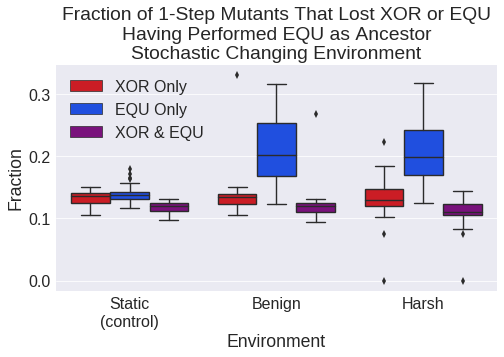
\includegraphics[trim={0.2cm 0 0 0.2cm},clip,width=0.75\columnwidth]{figures/CE/CSE_frac_1step__filtered__box.png}
	\caption{\textbf{A survey of the single-step mutational neighborhood} in the stochastic changing environment around organisms that performed the fluctuating task. Again, in the static and harsh treatments, values are comparable to the cyclic changing environment . However, in the benign treatment, the mean for the loss of the fluctuating task (\texttt{EQU}) was slightly higher in the stochastic treatment (Mdn = 0.2) than the cyclic (Mdn = 0.17), though the effect is barely statistically significant (Wilcoxon Rank-Sum Test: Z = -2.4, p = 0.015). This result indicates that stochastic environmental change is equivalently effective at moving organisms to areas of the fitness landscape where they can more easily switch task expression.%
	}\label{fig:CSE_single_step}
	\end{figure}
	\begin{figure}[!h] %% FIGURE 11
	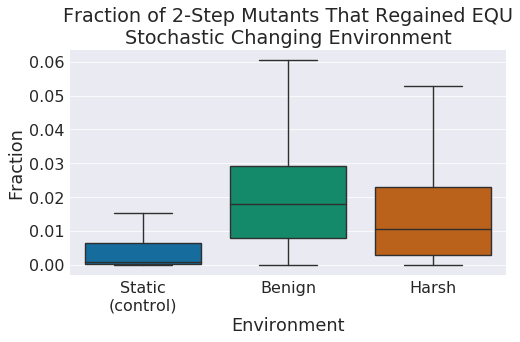
\includegraphics[trim={0.2cm 0 0.4cm 0.25cm},clip,width=0.75\columnwidth]{figures/CE/CSE_frac_2step__box.png}
	\caption{\textbf{A survey of the two-step mutational neighborhood} in the stochastic changing environment of the organisms that lost EQU function in the one-step survey. We found that the fraction of organisms regaining the fluctuating task (EQU) from a single additional mutation in the harsh treatment (Mdn = 0.013) were reduced compared to the cyclic harsh treatment (Mdn = 0.01) (Wilcoxon Rank-Sum Test: Z = 12.75, p $<<$ 0.0001) The opposite, however, was true of the Benign treatments. As in Fig~\ref{fig:CSE_single_step}, we find that stochastic outperforms cyclic (Wilcoxon Rank-Sum Test: Z = -18.43, p $<<$ 0.0001) This result confirms that the harsh stochastic environment is probably less effective than the cyclic harsh at promoting evolvability, but that the opposite may be true for a benign environment.
	}\label{fig:CSE_two_step}
	\end{figure}

%=discussion of function vs vestigial
Few differences between the cyclic and stochastic treatments also appeared in the number of functional and vestigial sites. Both the numbers of functional and vestigial sites in the stochastic environment were similar to those in the cyclic environment. In the stochastic harsh treatment, there was a small, but significant reduction in the number of XOR+EQU overlapping functional sites (Mdn = 14) as compared to the cyclic treatment (Mdn = 16) . (Fig~\ref{fig:CSE_func_vestigial}) 

%=[FIGURE - func vestigial sites]
%\todo[color=green]{stats}
	\begin{figure}[!h]
	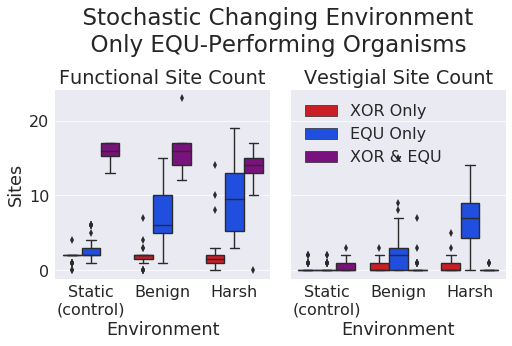
\includegraphics[trim={0 0 0 0}, clip, width=0.75\columnwidth]{figures/CE/CSE_func_vest__filtered__box.png}
	\caption{\textbf{Number of functional and vestigial sites by treatment} in a stochastic changing environment. The vestigial site counts for EQU-only remain comparable to the cyclic environment (Wilcoxon Rank-Sum Z = 0.46, 1.45, and -1.10, p = 0.6, 0.14, and 0.2). The functional sites were also comparable, however, there was a slight, but statistically significant decrease in the number of XOR \& EQU overlapping sites in the stochastic vs cyclic environments (Wilcoxon Rank-Sum Test: Z = -3.05, p < 0.01).
	%
	%-old (One-Way ANOVA F(2,132) = 54.35, p $<<$ 0.0001).
	}
	\label{fig:CSE_func_vestigial} %% FIGURE 9
	\end{figure}

%=hypothesyze these effect driven by variance in timespans
%We hypothesize that these effects were driven by the inconsistent time spans between the population experiencing a given environmental condition in the stochastic treatments. Especially long time spans without a reward for a task, even if rare, could allow vestigial sites to drift away, thus pushing subsequent evolution closer to the control treatment. However, due to the rarity of such events, the effects of drift would be relatively limited.
Together, from these measures, we conclude that stochastic environments exert similar evolutionary pressure to move toward regions of the mutational landscape that are more congenial to neutral phenotypic exploration and evolvability. However, the combination of the slight improvements in benign stochastic environments, matched by slight decreases in effectiveness in harsh stochastic environments, suggests that the periodicity of the cyclic environment provides a slight advantage to adapting to harsh environments. In the benign environments, however, the stochastic nature may be less of a disadvantage. We hypothesize that this dynamic may be due to the randomly-occurring environmental changes either occurring too rapidly for a response to selection, or too slowly, such that drift may cause the information contained in vestigial sites to mutate away. While the environment, on average, experiences as many changes as in the cyclic experiment, the distribution of the length of those environment periods may be very different. We conclude that our stochastic changing environment is not more effective than a cyclic changing environment, and under harsh conditions, may actually be slightly worse for promoting the evolution of evolvability.

%@CAO - If you want to talk about how to further explore this idea, you would probably do a range of runs with different cycle periods and show that the one we're using is somehow optimal. It might be that if we compared to a non-optimal cycle time, the stochastic would do better since it would sometimes bring changes into a more optimal range
%@RCK - One of my appendices recounts the runs we did to arrive at the 1000 update cycle time, so that wouldn't be a bad foundation for a comparison.

\section{Conclusion}
%=direction of selection drives exploration and gathers history
In cyclic changing environments, the direction of selection shifts frequently, and periodically drives populations to not only explore new regions of the genetic landscape, but also to carry with them vestigial genetic information about previous environmental conditions. Thus, the resulting populations are not only adapted to the current environment, but also to the meta-environment of cyclic change. Because of their evolutionary history, the genomes contain vestigial fragments of genetic material that were adapted to prior environments. As this exploration proceeds, mutations accumulate in the population, each creating a link to a new region of the mutational landscape. As these links accumulate, they form a reservoir of mobility for the population to quickly shift to new phenotypes as dictated by current selective conditions. In this way, the accumulation of vestigial or pseudogene-like regions acts as an indirect adaptation to the larger pattern of changing selective forces. 
%@CAO - This argument clearly implies that evolvability is not actually selected for. It's merely a by-product of how changing environments naturally alter genomes by creating genetic reservoirs. I feel like this is a point that we might want to hilight further.
%@RCK - agree. done.
Thus, architectural features that help with evolvabilty are the result of repeated hitchhiking on adaptive mutants.

%=by constrast static environments don't
By contrast, in static (non-changing) environments, the majority of neutral mutations do not connect to as many phenotypically-interesting regions of genotype-space. There are far fewer pseudogene-like regions available that could regain functionality should conditions change. Thus, populations evolved in static environments are less evolvable in the short-term.

%=SCE not more effective
Surprisingly, stochastically changing environments are not more effective at exploration
% @CAO: Are they really?  We've shown that they produce new phenotypes less often, but that's a very limited definition of exploration.  However, it's the one that we need to stick to.
% @CAO: That said (and this argument goes to static environments too), if we claim that stochastic environments produce new phenotypes less frequently we can argue WHY we hypothesize that they'll be less effective at exploration.  In thinking about it, it feels like we should use these as ancestors for an entirely new environmental shift.  If we show that the organisms previously experiencing a cyclically changing environment do better with the new environment THEN we have strong evidence that stochastically changing environments are less effective at exploration.
than cyclic changing environments, even if, on average, the amount of time spent in each environment was equal. We hypothesize that this result is because of more opportunity for drift to destroy the information contained in vestigial regions, as well as potentially fewer opportunities for populations to respond to selection.



%%%%%%%%%%%%%%%%%%%%%%%%%%%%%%%%%%%%%%%%%%%%%%%%%%%%%%%%%%%%%%%%%%%%%%%%%%%%%%%%%%%%%%%%%%%%%%
%%%%%%%%%%%%%%%%%%%%%%%%%%%%%%%%%%% CHAPTER 3 %%%%%%%%%%%%%%%%%%%%%%%%%%%%%%%%%%%%%%%%%%%%%%%%
%%%%%%%%%%%%%%%%%%%%%%%%%%%%%%%%%%%%%%%%%%%%%%%%%%%%%%%%%%%%%%%%%%%%%%%%%%%%%%%%%%%%%%%%%%%%%%


\chapter{Changing Environments and the Evolution of Horizontal Gene Transfer}
\label{chap:evo-hgt}
\section{Background}

%=HGT umbrella term
Horizontal Gene Transfer (HGT) is a broad term for the non-reproductive transfer of genetic material between organisms. Organisms may uptake genes directly from the environment (transformation via natural competence \cite{chen_dna_2004}), or else receive them via bacterial conjugation\cite{lederberg_gene_1946} or viral infection (transduction \cite{zinder_genetic_1952,lennox_transduction_1955}). In the case of transformation, the fragments may either be decomposed inside the recipient cell for their nutrients, or recombined into their genomes. 

%MJW: Being technical, just because this is a dissertation chapter:  The process by which organisms take up DNA directly is technically transformation; competence is the state of a cell capable of undergoing transformation.  You may or may not wish to mention gene transfer agents, which are essentially domesticated viruses encoded by certain types of bacteria -- their origins are viral, but they're now incorporated into the bacterial genome, and no longer capable of switching back to a viral lifestyle.
%@RCK: Corrected terminology

%=HGT profound impact
HGT has had a profound impact on the evolutionary history of both prokaryotes and eukaryotes, with one study showing approximately 81\% of genes in the sample "being involved in HGT at some point in their history" \cite{dagan_modular_2008}. For example, HGT appears to be the primary mechanism by which antibiotic resistance is conferred \cite{davies_origins_1997,martinez_antibiotics_2008} since most antibiotics are sourced from the environment, and the organisms that develop them are themselves resistant to the compounds.
However, the origins and evolution of HGT mechanisms remain unclear. 

\subsection{Origins of Horizontal Gene Transfer in nature}
\todo[inline, color=magenta]{More about how this question is still open}
% MJW: In line with your todo, you can hammer here the same thing I mentioned in your conclusions for this chapter -- it's really hard, and possibly even impossible, to test these things in non-digital systems.

%=natural competence in prokaryotes and why HGT happens
In prokaryotes, ''transformation'' is an HGT mechanism by which organisms spontaneously uptake the DNA of dead organisms in the environment. Competent organisms benefit in several ways. 1) DNA is composed of a 5-carbon sugar, a phosphate, and nitrogenous bases, materials that are useful for DNA synthesis and repair. 2) The organisms may also benefit from taking up
% MJW: You are inconsistent with hyphenation in uptake and up-taking.  I don't think you should have a hyphen here.
%@RCK: fixed everywhere it appears.
gene fragments that confer new adaptive functionality into the genome \cite{vos_why_2009}. However, it is unclear whether the origins of transformation functions were developed solely in order to obtain nutrients (the Grazing Hypothesis), or if the acquisition of new functionality was selected for as well. While grazing for gene fragments as nutrients certainly conveys an advantage, the possibility of integrating these gene fragments is likely to be deleterious to organisms more often than it is beneficial \cite{redfield_evolution_1997}. For example, since the DNA would be originating from dead organisms, DNA fragments may be of low quality, and recombine deleterious mutations, or even remove competence altogether \cite{redfield_evolution_1997}. Alternately, errors in homologous recombination may apply fragments to random locations in the genome.    
% MJW: I suggest expanding on this last sentence: why is it that integrating these fragments is likely to be disruptive more often than it is beneficial?  Also, how do either of those probabilities compare to it having no effect?
% @RCK: Added additional sentence explaining the reasoning from Redfield's paper for this claim.

%=statement of hypotheses - grazing CE elevates HGT
In order to test the Grazing Hypothesis,
% MJW: Identify what hypothesis you are testing.
%@RCK: fixed
, and address the question of whether there are circumstances where gene fragment 
% MJW: I don't think that gene fragment is hyphenated
%@RCK: fixed
integration may be beneficial, we subjected populations of evolving digital organisms to a harsh changing environment,
% MJW: For the dissertation, this is probably fine, since you have a chapter about changing environments immediately before this one.  For a paper, we'll need to define what we mean by a harsh changing environment -- it's pretty standard nomenclature in the field of people who look at changing environments, but not all readers will know it.
where there is a strong selective pressure to quickly switch phenotype. We supplied organisms with an instruction that performs Horizontal Gene Transfer (\texttt{HGT-Uptake}).
% MJW: I added the "(HGT)" because this is the first time you use the term.  However, I don't know if you'd rather include the specific command names, typeset in the way that we typically do for instructions.  But I think you either need an "(HGT)" or you need to the underline the appropriate captial letters, since you use the acronym in the last sentence of the paragraph.
% MJW: UPDATE: I now see an HGT before this, though used without defining the acronym.
%@RCK: fixed all
That is, the instruction triggers uptake of a genetic fragment from the environment, and there is a probability that, rather than metabolizing the fragment for a bonus to execution speed, the fragment will instead be homologously recombined into the organism's genome. We show that in harsh changing environments, without any kind of bonus, organisms increase use of HGT as compared to execution in a static environment.


\section{Methods}
In this chapter, we use Avida to test hypotheses about the origins of Horizontal Gene Transfer. 

\subsection{HGT in Avida}
%=HGT triggered by instruction, and uptakes
In Avida, HGT is triggered by the \texttt{HGT-Uptake} instruction that, when executed, attempts to uptake a genome fragment from the individual cell reservoirs in the environment. As organisms die in Avida runs with HGT enabled, fragments of their genomes will accumulate in reservoirs. The fragments in the reservoirs will deteriorate over time, with older genomes disappearing from the reservoir as new ones enter. Fragments for uptake will be randomly selected from the reservoir.  

\todo[inline]{look for and hunt down passive voice}
% MJW: I'll point out that the entire previous paragraph is passive voice. Because it's you, Rose, I offer that often the easiest way to test whether a sentence is passive voice is if you can append "by zombies" to the end of it.  "Fragments for uptake will be randomly selected from the reservoir...by zombies."  It's slightly tortured for a few of the sentences, but it's something that is likely to stick with you.
%=HGT uptake may recombine or be metabolized
%Upon uptake, there is a configurable probability that the fragment is not metabolized;
We have implemented a configurable probability that, when a fragment is taken up, it is not metabolized;
% MJW: This probability doesn't come into being upon uptake.  Maybe something more like "We have implemented a configurable probability that, when a fragment is uptaken (or, if you prefer, taken up), it is not metabolized;" (Since the rest of this chapter, at least, is being written in first person plural.  In reality, *you* implemented this, but it would be jarring to switch repeatedly between "I" and "we" within a chapter)
%@RCK: fixed
instead, homologous recombination may occur (Figure \ref{fig:hgtprocess}). We performed experiments to derive bonus levels, fragment sizes, and recombination probabilities to arrive at a maximum use level for the HGT instruction. See Appendix~\ref{appendix:hgt_sweep} for more details. 

%=HGT and homologous recombination
\todo{Citation TODOs}
For all experiments described in this chapter, we used a 10\% recombination probability. Please refer to Appendix~\ref{appendix:hgt_sweep} for more information about the selection of this probability value. We also required three instructions as the minimal homologous match length on either side of the fragment. Three instructions on either side of the fragment ($26^3$ unique sequences) approximates the number of unique values keyed by 7 nucleotides ($4^7$ unique sequences). For the purposes of homologous recombination in plasmid cloning in E. coli, 20bp is enough to assume identity\cite{jacobus_optimal_2015}.   

% MJW: Beyond merely citing something about number of nucleotides needed, I think it's worth explaining how we therefore chose 3 instructions in Avida.  26^3 is ~ 4^7, so if you're talking about an average of 300 nucleotides matching on each end, that would be way more restrictive than what we're doing.  A recent citation you can use is Optimal Cloning of PCR Fragments by Homologous Recombination in Escherichia coli by Ana Paula Jacobus and Jefferson Gross in PLOS ONE.  https://doi.org/10.1371/journal.pone.0119221  That one mentions in its abstract how 20bp is enough to assume identity.
%@RCK: Applied

\begin{figure}[h!]
\begin{center}
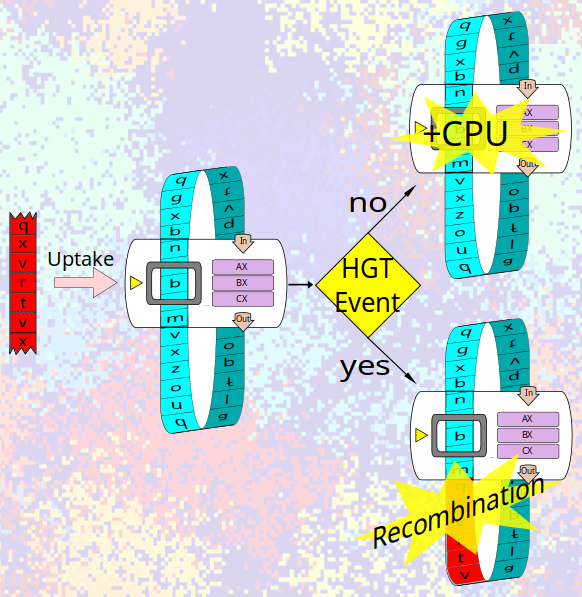
\includegraphics[width=0.7\columnwidth]{figures/HGT/hgt_figure.png}
\caption{\textbf{The HGT process}. Organisms can execute instructions that trigger uptake from the environment. When uptake occurs, there is an experimenter-defined chance that either it will yield a boost to speed of execution or, alternatively, that the fragment will be integrated into the genome.
}\label{fig:hgtprocess}
\end{center}
\end{figure}

\subsubsection{Environmental Conditions}
%=environmental rewards
All experiments in this chapter compare outcomes between static environments, and harsh changing environments. In a similar manner to the experiments listed in the previous chapter (Chapter~\ref{chap:ce-adaptation}, Table~\ref{ce-treatments-h}), task rewards in the harsh changing environment switch from a positive to a negative reward. For the HGT experiments, we did not establish a backbone task that was always rewarded. Rather, we divided the Logic-9 environment into two halves, and alternated positive and negative rewards for each task in each set. There are four pairs of tasks of equivalent complexity, and we randomly allocated one from each pair to an experimental group. We also assigned \texttt{EQU}, which is the most complex task, and has no equivalent, to a random group. Thus, for the first phase of the cycle, we punished the \texttt{NOT}, \texttt{AND}, \texttt{OR}, \texttt{NOR}, and \texttt{EQU} instructions at $-2^1$, $-2^2$, $-2^3$, $-2^4$, and $-2^5$ respectively, while rewarding \texttt{NAND}, \texttt{ORN}, \texttt{ANDN}, and \texttt{XOR} at $2^1$, $2^2$, $2^3$, and $2^4$. In the second phase of the cycle, these rewards flip, such that we reward \texttt{NOT}, \texttt{AND}, \texttt{OR}, \texttt{NOR}, and \texttt{EQU}, and punish \texttt{NAND}, \texttt{ORN}, \texttt{ANDN}, and \texttt{XOR}.

% MJW: I suggest explaining how you chose to divide the tasks; ie, there are 4 pairs of tasks of equivalent complexity, and for each pair you arbitrarily assigned one task to set 1 and the other task to set 2, and then EQU had to go somewhere.  Also, you can switch "were/are punished" with "we punished" and the like to remove passive voice.
%@RCK: fixed

%=cycle length
Each complete cycle lasts 1,000 updates, and the whole experimental run continues for 200,000 updates.

%=static environment
The static environment rewards executions of all the Logic-9 tasks at their default levels, with no reward switching.

% MJW: Why are the cycle length, static environment, and last sentence of the preceding paragraph in present tense, when the chapter in general is in past tense?

\subsection{Experimental Design}
%\subsubsection{Evolution of HGT - Alternatives to the Grazing Hypothesis}
%=we subject populations for testing the grazing hypothesis
For the treatments corresponding to the first set of hypotheses on the origins of horizontal gene transfer, we subjected four populations of evolving digital organisms with HGT to harsh changing environments (Table~\ref{hgt-treatments-h}), plus a fifth non-HGT control. The treatments correspond to the combination of two factors: static vs changing environment, and grazing bonus vs no bonus.

% MJW: You're switching between past and present tense again.

%=[TABLE - experimental treatments part 1]

\begin{table}[]
\centering
\caption{\textbf{Experimental Treatments - Evolution of HGT}}
\label{hgt-treatments-h}

\begin{tabular}{|c|c|c|c|}
\hline
\thead{Treatment} & \thead{Changing \\ Env. \\ Type} & \thead{HGT \\ Action} & \thead{Bonus} \\\hhline{|=|=|=|=|}
Control & Static & None & n/a \\\hline
\makecell{HGT \\ B0.0 \\ (Natural Competence \\ No Bonus)} & Static & \makecell{10\% \\ Recombination \\ Probability} & n/a \\\hline
\makecell{HGT \\ B0.0 \\ CE \\ (Natural Competence \\ No Bonus)} & \makecell{Harsh \\ Cyclic} & \makecell{10\% \\ Recombination \\ Probability} & n/a \\\hline
\makecell{HGT \\ B0.8 \\ (Natural Competence \\ with Bonus)} & Static & \makecell{10\% \\ Recombination \\ Probability \\ otherwise \\ Bonus \\ Allocation} & \makecell{$2^{0.8}$ per \\ Uptake} \\\hline
\makecell{HGT \\ B0.8 \\ CE \\ (Natural Competence \\ with Bonus)} & \makecell{Harsh \\ Cyclic} & \makecell{10\% \\ Recombination \\ Probability \\ otherwise \\ Bonus \\ Allocation} & \makecell{$2^{0.8}$ per \\ Uptake} \\\hline
\end{tabular} 

\begin{flushleft} Experimental treatments. Four treatments corresponding to the combination of two factors: Static vs Changing Environment, and Grazing Bonus vs No Grazing Bonus, plus a non-HGT control, where the HGT instruction is inert.  
\end{flushleft}
\label{hgt-treatments}
\end{table}

%=we test for the mechanisms of why CE promotes HGT
For the second set of hypotheses, where we identify the mechanisms that promote the use of HGT, we manipulate the content of the reservoirs to contain fragments drawn from specific phases in the cyclically changing environment, such that fragments either match or do not match the environment (Table~\ref{hgt-treatments-h-reservoir}. We then measure HGT use, as well as average fitness effects of the HGT mutations, and the fraction of mutations that lead to beneficial phenotype switches.

%=[TABLE - experimental treatments]
\todo{rename table}
\begin{table}[]
\centering
\caption{\textbf{Experimental Treatments - Effects of HGT}}
\label{hgt-treatments-h-reservoir}

\begin{tabular}{|c|c|}
\hline
\thead{Treatment} & \thead{Fragment\\Source} \\\hhline{|=|=|}
HGT & organism death \\\hline
\makecell{HGT-Both} & sampled from organisms from both phases \\\hline
\makecell{HGT-OnPhase} & sampled from organisms from the matching phase \\\hline
\makecell{HGT-OffPhase} & sampled from organisms from the non-matching phase \\\hline
\end{tabular} 

\begin{flushleft} Experimental treatments. Four treatments corresponding to the sources of fragments. The first treatment uses the default fragment source (dead organisms from the environment). The second treatment samples a population for organisms corresponding to both phases, and injects those into the reservoirs. The third and fourth treatments sample the population, but only inject fragments from the matching and non-matching phases, respectively.  
\end{flushleft}
\label{hgt-treatments-reservoir}
\end{table}


\section{Results and Discussion}
\todo[inline]{clarify whether a summary paragraph like this is even useful. or if it should be framed differently}
Our results show that both an uptake bonus and changing environment promote the use of HGT, and that the increases in uptake are largely additive. Further, we found that while on average, HGT mutations are neutral, that the majority of the benefits conveyed by HGT in changing environments come from fragments originating in periods of the cycle where the environment matched the current environment. This result indicates that it is the information content of the fragment that is valuable. Finally, we find that providing only fragments from the matching cycle elevates uptake rates significantly.
% MJW: This paragraph is essentially a bunch of numerical claims with no stats.  I'll be on the lookout for stats in the coming results -- I didn't see a statistical methods section in the methods -- but if they don't exist we need them; if they do, we probably want some sort of "(see below)".
%@RCK: It's intended as the tip of the pyramid type summary paragraph. Should I even have something like this?

%\subsection{Alternatives to the Grazing Hypothesis}
\subsection{Changing environments elevate HGT use}
%Measured HGT fragment uptake in four conditions - 0Static, BStatic, 0CE, BCE.
%* No bonus, static - uptake remains low
%* Bonus, static - uptake increases
%* No bonus, CE - uptake higher than no bonus static
%* Bonus, CE - uptake higher than either BonusStatic or NoBonusCE

%=measured fragment uptake, results summary
We measured HGT fragment uptake in four conditions (see Table~\ref{hgt-treatments-h}), plus of pair of non-HGT controls. Without a bonus, in a static environment, fragment uptake is depressed to a low level as compared to the rate of the non-HGT control, where the \texttt{HGT-Uptake} instruction does nothing. This indicates that HGT in a static environment is largely deleterious (Figure~\ref{fig:hgt_inst_execution}). However, in a harsh changing environment, fragment uptake is elevated. This shows that in the context of a harsh changing environment, the integration of new genetic material is more beneficial than in the static environment. We also found that, regardless of whether the environment is static or changing, when a bonus to fragment uptake is provided (analogous to the nutritive benefit granted by natural competence in biological organisms), fragment uptake also increases. 

%=measured fragment uptake wrl to bonus
In order to investigate the relationship between the effects granted by a nutritive bonus and the benefit of fragment recombination in a changing environment, we selected a bonus level that increased fragment uptake in a static environment to a level comparable to the increase seen in changing environments without a bonus. We then combined these factors, giving a bonus, plus using a changing environment. We saw that the resulting uptake level increases largely additively. This indicates that the benefits granted by a grazing bonus are largely independent of the benefits conveyed by integrating new genetic material. 
% MJW: The preceding paragraph reads like methods, no?
%@RCK: Eh. I don't know. It's what we measured. Yes, we did a specific experiment, so that should be documented in methods. But I don't mind explaining the measure here.
\todo[inline]{document the additive measuring thing in methods, per note}

%We thus conclude that not only is HGT evolution possible absent a grazing bonus, but that should a changing environment occur, that there are additional incentives to perform HGT.
%=conclusion sentence - hgt is promoted by HGT
Thus, not only is HGT evolution possible absent a bonus, the benefit stacks with that of a grazing bonus, proving a more likely scenario by which HGT might evolve. %bleh

\todo[color=green]{stats}
% MJW: Ding ding ding!  :)
\begin{figure}[h!]
\begin{center}
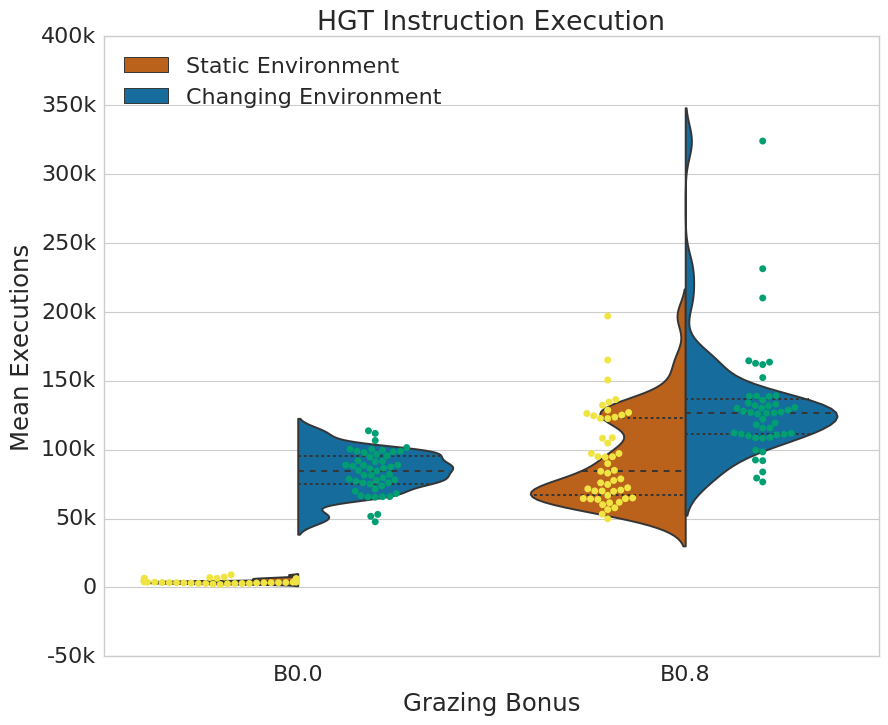
\includegraphics[width=0.7\columnwidth]{figures/HGT/hgt_inst_execution.png}
\caption{bleh%\todo{stats}\todo{caption}
}\label{fig:hgt_inst_execution}
\end{center}
\end{figure}




\subsection{HGT derives most benefit from on-cycle fragments, but not all}
%Measured fitness effects of HGT fragments that originated in a matching phase in a previous cycle vs fragments originating in the non-matching phase of the cycle.

%=understanding why HGT is used
In order to understand the basis of the beneficial nature of HGT in changing environments, we performed a series of treatments where we replaced the fragments in the cell reservoirs with fragments that originated at the end of the matching phase of the cycle, the off-phase of the cycle, and from both phases, plus a non-replaced control. (Figures~\ref{fig:fitness_effect_heatmap}, \ref{fig:hgt_use_by_cycle_phase_source}, \ref{fig:fitness_effect_by_cycle_phase_source}, \ref{fig:beneficial_fraction_by_cycle_phase_source})
We then measured the levels of HGT use, the fitness effect of HGT mutations, as well as the fraction of beneficial phenotype-switching mutations. In the both-phase and non-replaced control, the mean fitness effect was largely neutral, while the on-phase fragments had a significantly positive mean fitness benefit as compared to both the both-phase and non-replaced controls\todo{stats}. The off-phase fragments were largely negative when compared to the both-phase and non-replaced controls\todo{stats}. Further, the control, both-phase and on-phase all had a larger fraction of beneficial phenotype-switching mutants
% MJW: compared to what?  Than other treatments?  Than non-beneficial phenotype switches?  Than mutations which don't switch phenotypes? I don't actually know what comparison you're making here.
than the the off-phase treatment, which had few to no beneficial phenotype switches\todo{stats}. This indicates that it is not only genetic disruption that is beneficial, but that the majority of the benefit of HGT derives from taking up and integrating useful fragments of information from time-periods where organisms were already adapted to the environment, thus bypassing the need to evolve a new phenotype from scratch.

\subsubsection{Expected Fitness Effects}

%=measured fitness effect in normal HGT
We calculated the average fitness effects of fragments in a randomly selected replicate of the non-replaced HGT control treatment at the end of the last environmental cycle, and generated a distribution of fragments sorted the fragments by age and fitness-effect (Figures~\ref{fig:fitness_effect_heatmap}). We can see a clear pattern of more beneficial fitness effects from fragments of organisms originating in the matching cycle phase. 
% MJW: Have we done this for only one replicate?
%@RCK: yes. It's an example of what they look like. Maybe we don't care that they look this way, but I like the figure :P

\todo[color=green]{stats}
\begin{figure}[h!]
\begin{center}
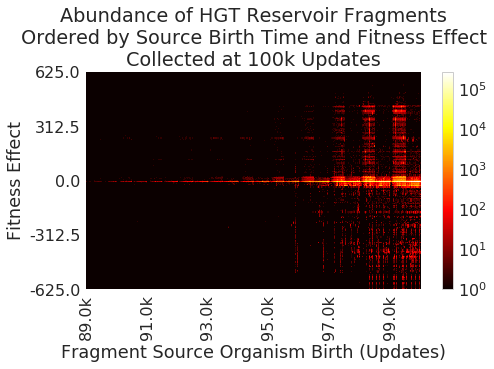
\includegraphics[width=0.7\columnwidth]{figures/HGT/fitness_effect_heatmap.png}
\caption{bleh%\todo{stats}\todo{caption}
}\label{fig:fitness_effect_heatmap}
\end{center}
\end{figure}

%=manipuated reservoir to match or not match phase - measured effects 
In order to quantify this result, we performed experiments where we replaced the fragments in the reservoir to contain only fragments originating in the matching phase, the off-phase, and mixture of both phases. We measured the mean fitness 
% MJW: Why "expected" fitness?
%@RCK: fixed
effects of fragments in these treatments (Figure~\ref{fig:fitness_effect_by_cycle_phase_source}). We found that HGT mutations are, on average, neutral in both the non-replaced control and the replaced-"both" treatment. The average fitness effect in the "on-phase" treatment was mildly beneficial, while in the "off-phase" treatment, the effect was strongly deleterious\todo{stats}. 

\todo[color=green]{stats}
\begin{figure}[h!]
\begin{center}
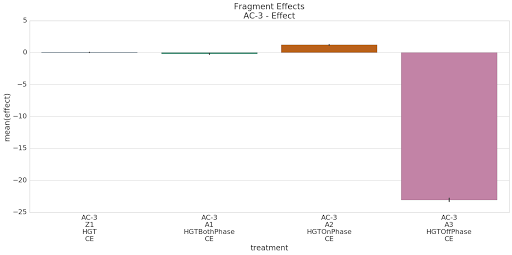
\includegraphics[width=0.7\columnwidth]{figures/HGT/fitness_effect_by_cycle_phase_source.png}
\caption{bleh%\todo{stats}\todo{caption}
}\label{fig:fitness_effect_by_cycle_phase_source}
\end{center}
\end{figure}

%=measured phenotypic change
In our environments, mutations that convey phenotypic change should have the largest impact. Specifically, the largest fitness benefits should occur when a mutation leads to the acquisition of a new rewarded task, or the loss of a punished task.  
% MJW: Slightly redundant; you just specified which pheotypic changes have the largest impacts, and then said that things that result in phenotypic changes have the largest impacts.  If you change the order of these sentences, you can put the "In our environments" on what is currently the second sentence, and then lead in with "Specifically, " for what is currently the first sentence.
%@RCK: fixed
We quantified 
% MJW: Isn't this quantification, not identification?
%@RCK: fixed
the phenotypic effect of each fragment by counting the number of times that fragments produced a beneficial phenotype change, vs all HGT mutations (Figure~\ref{fig:beneficial_fraction_by_cycle_phase_source}). We see that a significantly larger proportion of fragments in the "on-phase" treatment produce beneficial phenotype changes, as compared to fewer in the normal HGT and "both" treatments, and virtually zero in the "off-cycle" treatment\todo{stats}. 

\todo[color=green]{stats, caption}
\begin{figure}[h!]
\begin{center}
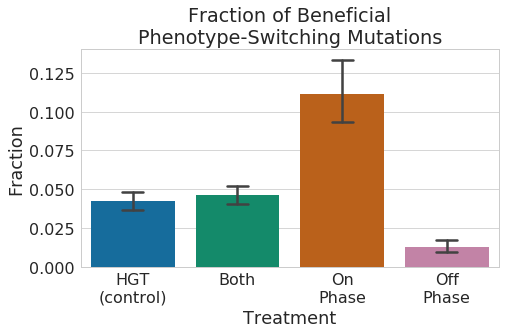
\includegraphics[width=0.7\columnwidth]{figures/HGT/beneficial_fraction_by_cycle_phase_source.png}
\caption{bleh%\todo{stats}\todo{caption}
}\label{fig:beneficial_fraction_by_cycle_phase_source}
\end{center}
\end{figure}

%=benefit results from matching environment and information conveyed
These results suggests that any direct benefit of using HGT derives from taking up fragments that match the cycle phase of the environment of the affected organism, and thus likely contains information that relates to that environment. %otherwise, it wouldn't matter where the fragment came from

%=see uptick in use when fragments match phase only.
Further, if fragments from the matching phase are indeed beneficial, we would expect to see an increase in HGT use in those treatments, as compared to those where the fitness effects are mixed or deleterious. And indeed (Figure~\ref{fig:hgt_use_by_cycle_phase_source}), we do observe just such an increase. Thus we can conclude that HGT in our
% MJW: I suggest adding the word "our" here; it's hard to conclude that this is a universal from studying one system.
%@RCK: fixed
changing environments is most beneficial when the fragments in the environment contain information that would be beneficial in that environment. However, even when no such information is available, HGT use is not significantly depressed as compared to the control treatment. This suggests that despite the lack of exclusively matched environmental information, that fragments could still provide some benefit. 

\todo[color=green]{stats}
\begin{figure}[h!]
\begin{center}
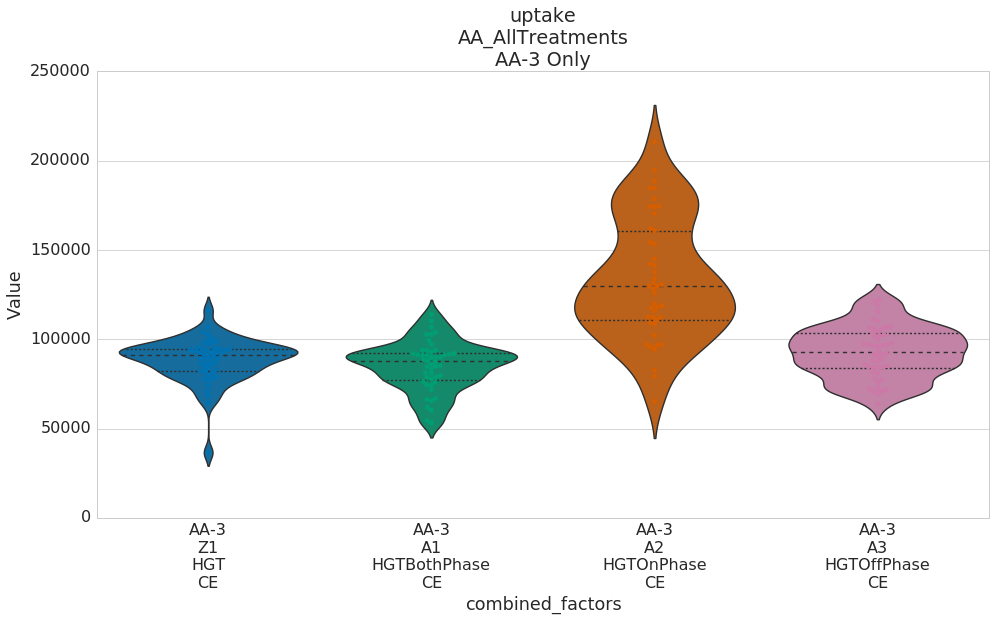
\includegraphics[width=0.7\columnwidth]{figures/HGT/hgt_use_by_cycle_phase_source.png}
\caption{bleh%\todo{stats}\todo{caption}
}\label{fig:hgt_use_by_cycle_phase_source}
\end{center}
\end{figure}


%%%%%%%%%% EXTRA SECTION IF HAVE TIME
%\subsection{Information content of fragments predicts HGT benefit}
%\todo[inline, color=magenta]{fill this in - info theory predicts HGT benefit}
%%%%%%%%%%%%%%%%%%%%%%%%%%%%%%%%%%%%%%%

\section{Conclusion}
%@CAO - Start with a comment along the lines of Avida confirming our expectations about HGT, and matching what we'd expect to see in natural populations.
% CE selects for evolvability 
% * When sufficiently beneficial mechanisms exist, and 
% * When change is directly selected for, as in a changing environment
% * Because HGT is much more beneficial than other types of mutation
% Under Stress, Natural Competence increases
% * In natural organisms, Natural Competence tends to be up-regulated, and recombination rates increase [cite]. 
% * This effect may occur because of loss of fidelity of DNA copying and repair mechanisms due to stress. 
% * Avida has no such mechanism, so lack of fidelity does not account for an increase in HGT use. Instead, HGT can only increase due to selection. 
Our experiments confirm our expectations about the evolution of horizontal gene transfer, and match what we would expect to see in nature. First, we find that grazing bonuses, such as those conveyed by the uptake of nutrient-rich DNA fragments in natural systems, cause an elevation of use of the horizontal gene transfer instruction, regardless of the potential risk of recombining uptaken gene fragments. 

Further, when there is direct selection for phenotypic change - such as in a changing environment - we observe an increase in the use of the HGT instruction, even when no grazing bonus is offered. This indicates that the possibility of recombination itself is being selected for. Beyond this, we find that it is not only the fact of the recombination that is beneficial, but the information contained in the fragment. We found that 
% MJW: "not only" is getting a bit repetitive.  
%@RCK: fixed
most of the benefit conveyed by HGT derived from fragments that match the current environment, but also that when we filter so that only those fragments are available, that use of the HGT instruction increases even further. 

In natural systems, this pattern in evident in the acquisition of antibiotic resistance in bacteria, where resistance is acquired by the spread of resistance genes via horizontal gene transfer. Therefore, our results provide a key insight into how horizontal gene transfer mechanisms could be selected for, and evolve in natural systems.

\todo[inline]{review the below. too strong? too informal?}
It is worth noting that most prior studies of HGT have been observational studies that look at existing traits and phylogenies and attempt to make inferences about the evolution of those traits on that basis. Performing experimental evolution studies of the evolution of HGT in organic systems is something that, to a first approximation, we simply can't study in a wet system. Digital evolution, on the other hand, allows us to test many hypotheses about the evolution of HGT, such as the explicit benefits and consequences of different types of mutations, as well as gives us an opportunity to compare granular fragment grazing bonuses and quantify their effects on evolutionary outcomes. These are experiments that we would not be able to perform any other way.   
% MJW: I suggest explicitly making what probably seems like a really obvious point: Digital systems like Avida let us test things -- like the benefits and consequences of certain types of mutations being allowed -- in ways that are essentially impossible in organic systems.  This is something that, to a first approximation, we *can't* study in a wet system -- we can't create otherwise-identical systems in which one has HGT as a possibility and the other doesn't.  If we want experimental results to test theoretical predictions, digital systems are arguably the best way to do this -- any wetlab system would involve other differences between the environments too.
%@RCK: Added something to that effect. Somebody give it a read-over?

%%%%%%%%%%%%%%%%%%%%%%%%%%%%%%%%%%%%%%%%%%%%%%%%%%%%%%%%%%%%%%%%%%%%%%%%%%%%%%%%%%%%%%%%%%%%%%
%%%%%%%%%%%%%%%%%%%%%%%%%%%%%%%%%%%%%%%%%% CHAPTER 4 %%%%%%%%%%%%%%%%%%%%%%%%%%%%%%%%%%%%%%%%%
%%%%%%%%%%%%%%%%%%%%%%%%%%%%%%%%%%%%%%%%%%%%%%%%%%%%%%%%%%%%%%%%%%%%%%%%%%%%%%%%%%%%%%%%%%%%%%

\chapter{Horizontal Gene Transfer vs Other Types of Mutation}
\label{chap:hgt-preferred}
\section{Background}

In both natural and artificial systems, populations evolve mechanisms to reduce or eliminate mutation\cite{wielgoss_mutation_2013}, despite evidence that higher mutation rates may be optimal\cite{clune_natural_2008}.
% MJW: Possible citations: Jeff Clune's Avida work on reduction in mutation rate; Wielgoss et al 2013 PNAS paper that shows two independent clades in one of the LTEE populations that reduce the mutation rate in the hypermutator background.
%@RCK: applied
In artificial systems, prior research has failed to show an increase in endogenously-controlled mutation rates, when such an increase would be beneficial for long-term evolution, such as in a changing environment\todo{[TODO CITE]}. However, Horizontal Gene Transfer through transformation seems to be exception to this rule.  
% MJW: I don't think natural competence is capitalized, either here or in the next sentence.

%Why should HGT mutations be different? 
In nature, transformation is a highly regulated and refined mechanism for taking up DNA fragments from the environment \cite{solomon_whos_1996,seitz_cues_2013,fontaine_novel_2010}. 
% MJW: Here are the DOIs for some citations: https://doi.org/10.1016/0168-9525(96)10014-7 ,  https://doi.org/10.1111/j.1574-6976.2012.00353.x , and also a 2009 J of Bacteriology paper titled A Novel Pheromone Quorum-Sensing System Controls the Development of Natural Competence in Streptococcus thermophilus and Streptococcus salivarius
%@RCK: applied
Clearly, evolution
% MJW: Why use natural as an adjective here?
%@RCK: removed
is acting to maintain and preserve these functions, despite the risk of bad recombinations. In the previous chapter, we showed that HGT is directly selected for in harsh changing environments. Despite the neutral to slightly deleterious fitness effects of recombination, HGT use is upregulated.
% MJW: I don't think there is a hyphen here.
%@RCK: removed hypen
What makes HGT different from other types of mutations?
% MJW: Pretty sure you mean mutation.
%@RCK: fixed
Is it the fitness effect? The information content of fragments? The probability for beneficial phenotype changes? 
% MJW: Maybe probability instead of potential?  I mean, pretty much any mutation has the *potential* to have a beneficial phenotypic change...
%@RCK: changed
How does HGT compare to other types of mutations in these respects?
% MJW: I think you mean mutation here too.
%@RCK: fixed
Can these differences account for the increased selection for HGT? 

In order to address these question, we created instructions that create different kinds of mutational effects with similar per-instruction impact to HGT. We then performed experiments with these mutagenic instructions under the same conditions as our evaluation of HGT, in static vs. changing environments. We found that not only are these instructions are triggered at significantly lowered rates as compared to HGT, but that the use rate correlates significantly with the amount of useful information conveyed by the mutation. 


\section{Methods}
In this chapter, we use Avida to compare mutational effects of HGT to other types of mutations. As in the previous chapter, HGT is triggered by the \texttt{HGT-Uptake} instruction, and fragments are uptaken from reservoirs in the environment. 

All experiments in this chapter compare outcomes between static environments and harsh changing environments. Similarly to the experiments in the previous chapter, task rewards in the harsh changing environment switch from a positive to a negative reward between the divided set of tasks in the Logic-9 environment. Please refer to Table~\ref{hgt-treatments-h} for more details. Each complete cycle lasts 1,000 updates, and the whole experimental run continues for 200,000 updates.
% MJW: I think if you use the comma for 200,000, you probably need it for 1,000 too.
%@RCK: fixed
Also as in the previous chapter, the static environment rewards executions of all the Logic-9 tasks at their default levels, with no reward switching.
% MJW: I think in most Avida work, Logic-9 is hyphenated
%@RCK: fixed everywhere

\subsection{Experimental Design}

\subsubsection{Alternative Mutagenic Instructions}
% MJW: I think this paragraph is mutations, not mutagens, again.
%@RCK: fixed
In order to perform experiments comparing HGT to other types of mutagens, we modified the functioning of the HGT instruction to perform a new set of mutagenic functions which should have the same raw, per-instruction effect as the normal HGT instruction. All mutagens have the same 10\% execution probability and viable recombination site requirements as the default HGT instruction.

\begin{itemize}
	\item \textbf{HGT (Intact Fragment)}: The default HGT operation. We uptake a fragment from the environment. We apply a 10\% probability that the fragment is recombined into the organism's executing genome. The recombination occurs homologously - that is, three instructions at the beginning and end of the fragment must match exactly with locations on the genome. We use the first valid match. We find valid matches by selecting a random location on the genome, then search from there. We loop around the whole genome, past the end and into the beginning, until we find a for the front three instructions of the fragment. Then, we begin searching for a match for the back three instructions of the fragment, starting at the edge of the front match. If a valid back-end match site is not found, we scan forward, looking for the next front-end match and repeat the process until all possible match sites on the genome are exhausted.
% MJW: What, exactly, does this mean?  Do you start from a random place in the genome and find the first match?  Do you always start at position 1 (or 0, I suppose) and find the first match, which would bias you towards recombining earlier in the genome?  Can the matching three bases span across the first and last instructions?  Also: you probably want "valid", not "viable", since we use viable to mean something specific in Avida.  This applies to several of the other items in this list too.
%@RCK: clarified to show random starting point, searching
If no match is found, the recombination fails. If recombination succeeds, it replaces the content between the selected beginning and end match sites. This may result in the genome growing or shrinking, depending on the distance between the matches, and the length of the fragment.
% MJW: Likewise here.  When searching for a match for the end of the fragment, do you always start from, say, exactly where the front edge perfect match stops?  Is there some formula that determines the first point at which you search for something? Do you assign all of the sites in the host genome a number, randomly permute that list of numbers, and then try each of them in turn as the starting point for a possible perfect match?
%@RCK: yes, we start looking for the back-end match at the edge of the front match. We loop all the way around the genome looking for a viable spot.
	
	\item \textbf{HGT Shuffle}: We uptake a fragment from the environment, and a valid recombination site is found, as above.
% MJW: I assume the same way as in the base?  Probably best to just say that.  Repeat this comment for the rest of the entries.
%@RCK: fixed
Prior to recombination, we shuffle the fragment, with the order of each instruction randomized. We then insert the fragment at the selected site.
% MJW: I suggest being more explicit about what you mean by shuffled.  Even if it's just "such that the inserted fragment has the exact same instructions as the originally chosen fragment, but the order of those instructions has been randomized".  Except that that, like this existing bit, is passive voice.
%@RCK: fixed
	\item \textbf{HGT Random}: We uptake a fragment from the environment, and find a valid recombination site, as above. Prior to recombination, we entirely replace the fragment with an equal number of randomly selected instructions, and insert it at the selected site.
    % MJW: Passive
	%@RCK: fixed
	\item \textbf{Mutation Event - Sampled}: We uptake a fragment from the environment, and find a valid recombination site, as above. Rather than recombine, we apply a number of point mutations in random locations throughout the genome. The number of applied mutations matches the number of instructions in the fragment. The mutations applied are sampled, with replacement, from the selected fragment. This mutagenic instruction is analogous to the the \textbf{HGT Shuffle} mutagen, except that instead of having a shuffled fragment be applied in a single location, the instructions from the fragment are sampled and applied randomly throughout the genome.
    % MJW: Sampled with no modifiers generally implies "with replacement". So if, say, the fragment were xgds, one possible result would be 4 new mutations in the genome: x, x, d, s (no g).  This may be what you did, but I want to be sure that it is.
	%@RCK: clarified, sampled with replacement

	\item \textbf{Mutation Event - Random}: We uptake a fragment from the environment, and find a valid recombination site, as above. Rather than recombine, we apply a number of random point mutations, matching the number of instructions in the fragment. This mutagenic instruction is analogous to the \textbf{HGT Random} mutagen, except that, again, its effects are applied randomly throughout the genome instead of at a single location.
    % MJW: I think these are mutations again, not mutagens.
    %@RCK: fixed

	\item \textbf{Mutation Rate Increase}: We uptake a fragment from the environment, and find a valid recombination site, as above. Rather than recombine, we increase the point-mutation rate for the organism, such that it will experience an expected additional number of point mutations matching the number of instructions in the uptaken fragment.
    % MJW: Is it that the it will experience this number of mutations, or that the expected number of mutations will be equal to the fragment size?
    %@RCK: expected. clarified.

	\item \textbf{Die}: We uptake a fragment from the environment, and find a valid recombination site, as above. Rather than recombine, the organism dies.	
    % MJW: Why find a valid recombination site, if you're just going to kill it?  Is it that if it fails to find a valid site, this doesn't kill the organism?
    %@RCK: Yup. We want to be able to compare the use rates, and that has to include all the times that instructions could and do fizzle.
\end{itemize}	

\subsubsection{Comparing HGT to Other Mutation Types}

For the experiments comparing the mutational effects of different types of mutations, we provided populations of evolving digital organisms with instructions that endogenously trigger different kinds of mutation events (see above), then subjected them to both static and harsh changing environments (Table~\ref{hgt_mut-treatments-h}).  

%=[TABLE - experimental treatments]
\begin{table}[]
\centering
\caption{\textbf{Experimental Treatments - Mutation Types}
}
\label{hgt_mut-treatments-h}

\begin{tabular}{|c||c|c|}
\hline
\thead{Treatment} & \thead{Environment} & \thead{Mutagenic Instructions} 
% MJW: I think these are mutations again.
%@RCK: fixed
\\\hhline{|=|=|=|}
HGT & Static & \multirow{2}{*}{ HGT } \\\cline{1-2}
HGT CE & Changing & \\\hline
HGT-Shuffle & Static & \multirow{2}{*}{ \makecell{HGT-Shuffle} } \\\cline{1-2}
HGT-Shuffle CE & Changing & \\\hline
HGT-Random & Static & \multirow{2}{*}{ \makecell{HGT-Random} } \\\cline{1-2}
HGT-Random CE & Changing & \\\hline
ME-Sampled & Static & \multirow{2}{*}{ \makecell{Mutation Event - Sampled} } \\\cline{1-2}
ME-Sampled CE & Changing & \\\hline
ME-Random & Static & \multirow{2}{*}{ \makecell{Mutation Event - Random} } \\\cline{1-2}
ME-Random CE & Changing & \\\hline
MRI & Static & \multirow{2}{*}{ \makecell{Mutation Rate Increase} } \\\cline{1-2}
MRI CE & Changing & \\\hline
Die & Static & \multirow{2}{*}{ \makecell{Die} } \\\cline{1-2}
Die CE & Changing & \\\hline
\end{tabular} 

\begin{flushleft} Experimental treatments. Two types of environment (static vs changing environment), for each mutagen. No bonus was given for performing any of the mutagen instructions.
\end{flushleft}
\label{hgt_mut-treatments}
\end{table}

%\todo[inline, color=magenta]{TODO - more discussion of what each treatment is intended to cover.}
The goal of each treatment is to compare the use rates of each of the different mutagenic instruction across several factors. We can examine the effects of localization (concentrating mutations in a single area) by comparing the \texttt{HGT-Random} vs the \texttt{ME-Random} treatments. We can measure the effect of time-concentration (all mutations happening at once vs spread out over time) by comparing the \texttt{ME-Random} and \texttt{MRI} treatments. We can examine the effect of information content by comparing the \texttt{HGT}, \texttt{HGT-Shuffle}, and \texttt{ME-Sampled} treatments. We can identify a basement-level for mutagenic instruction use by comparing against the use of the entirely deleterious \texttt{Die} instruction.  Finally, we can compare all these factors with their environment by comparing the static vs changing environment treatments.

\section{Results and Discussion}
Our research shows that only mutations containing useful information are elevated in response to changing environments. Intact-fragment HGT is used most, with shuffled-fragment (\texttt{HGT-Shuffle}) used less, and the other, non information-bearing mutagen types used at the lowest levels.  Further, we find a positive correlation between expected fitness and mutagenic instruction use. That is, mutagenic instructions that have higher expected fitness effects are used more. Finally, we see a strong positive correlation between the fraction of mutations from a mutagenic instruction that provides a beneficial phenotype-altering change, and the use of that instruction.
% MJW: I still think these are mutations, not mutagens.
%@RCK: fixed

\subsection{Other mutation types are not elevated in response to HGT}
% Measured use of mutagen instruction in static and changing environments
In order the compare the use of HGT against other kinds of mutation, we compared rates of non-bonus HGT fragment uptake against a execution of series of other mutation types, in both static and changing environments.\ref{fig:mutagen_execution} As expected, in the static environment, endogenously-controlled performance of all types of mutation (including HGT) is strongly suppressed. However, in harsh changing environment, HGT use dominates the other mutation types. Of particular interest is how the use of the HGT-like instructions are used most by order of information content. The intact-HGT instruction is used most, followed by the \texttt{HGT-Shuffle} instruction, and then followed by {HGT-Random}, where no information remains.\todo{stats}
% MJW: I don't know what you mean by "first" and "and then", since both commands presumably don't exist in the same treatment.
%@RCK: clarfied
The latter performs comparably to the remaining mutation types: Mutation Events: \texttt{ME-Sampled}, \texttt{ME-Random}
% MJW: You don't have anything currently called Mutation Event: Biased.  I assume this is the Sampled one?
%@RCK: fixed
, \texttt{MRI} (Mutation Rate Increase), and the \texttt{Die} control.\todo{stats} This indicates that the information content of the fragment is an important predictor of the use of HGT. 

Also of note is that the only difference between the \texttt{ME-Sampled} and \texttt{HGT-Shuffle} treatments is the localization of the mutation effect
% MJW: This statement strongly implies that the Sampled is "Without replacement".
(\texttt{HGT-Shuffle} fragment insertion is applied to a single location, whereas with \texttt{ME-Sampled}, the instructions are scattered randomly throughout the genome), however their use rates are significantly different. This indicates that not only is information content important, but that localization (clustering) of the mutation effect also matters.
% MJW: Consider expanding on this with speculation as to why it might matter.
%@RCK: speculated :)
We speculate that this effect may synergize with the level of modularity in a genome. If a genome is even slightly modular, there are gradients of relatedness between loci that decrease with physical distance. A single mutation is enough to disrupt a function. Thus, if all mutations are concentrated in one region, they would be more likely to affect fewer total functions.  Thus, concentrating mutations to a single area may limit the reach of the damage, so to speak, as opposed to hitting many different locations at once. We would expect this effect to increase as modularity of a genome increases.
%This indicates that a combination of information content and localization of the mutation event matter for the beneficial nature of HGT.

\todo[color=green]{stats}
\todo{caption}
\begin{figure}[h!]
\begin{center}
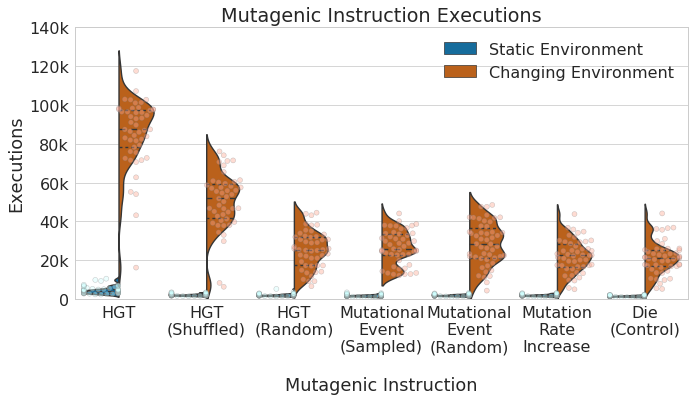
\includegraphics[width=0.7\columnwidth]{figures/HGT/mutagen_execution.png}
\caption{bleh
}\label{fig:mutagen_execution}
\end{center}
\end{figure}



\subsection{Mutation fitness effect correlate with mutagen use}
% Measured HGT fragment uptake in four conditions - 0Static, BStatic, 0CE, BCE.
% * Measured fitness effects of different types of mutagens
%   * Spatially-Dispersed Mutation Event
%   * Localized Mutation Event
%   * Shuffled-Fragment HGT
%   * HGT
%   * CE

Prior research has failed to show an increase in endogenously-controlled mutation rates, when such an increase would be beneficial for long-term evolution, such as in a changing environment\cite{clune_natural_2008}.
% MJW: This sentence demands citations.  Presumably Jeff Clune's Avida work?
%@RCK: fixed
Why should HGT mutations be different? In order to address this question, we measured the average fitness effect of each mutation, and compared it to that mutation's usage rate in changing environments. We observed a positive correlation between the average fitness effect, and the use of the mutagenic instruction\todo{stats}. We observed many more positive or neutral fitness effects from HGT-like instructions than the other mutagenic instruction types, which exhibited primarily neutral or negative mutation effects. This indicates that mutagenic instruction use is under direct selection (Fig~\ref{fig:mutagen_use_vs_fitness_effect}).
% MJW: I think these are mutations, again.

\todo[color=green]{stats}
\todo{caption}
\begin{figure}[h!]
\begin{center}
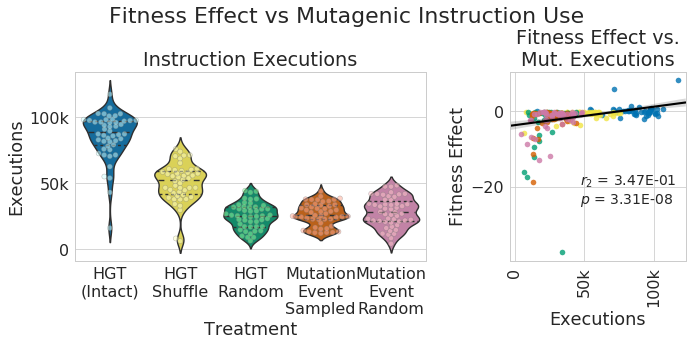
\includegraphics[width=0.7\columnwidth]{figures/HGT/mutagen_use_vs_fitness_effect.png}
\caption{bleh
}\label{fig:mutagen_use_vs_fitness_effect}
\end{center}
\end{figure}

%Fitness effects correlate with use of the mutagen.

\subsection{HGT mutations increase evolved probability of beneficial phenotype switching}
% Measured proportion of mutations that convey beneficial phenotype change (with an increase in fitness) for different types of mutagens
% * Spatially-Dispersed Mutation Event
% * Localized Mutation Event
% * Shuffled-Fragment HGT
% * HGT

%Further, 
% MJW: I would recommend against starting the first sentence of a section or subsection with "Further", since the break pushes that antecedent substantially further away.
%@RCK: fixed
We measured the proportion of mutations that produce beneficial phenotype changes.\ref{fig:mutagen_use_vs_fraction_beneficial} In the context of a changing environment, a mutation that switches an organism's phenotype to match the environment should be strongly selected for. Indeed, we found that this proportion was significantly and substantially higher for HGT-like mutations than other mutation types\todo{stats}, and that there was strong correlation between the proportion of beneficial phenotype-switching mutations and mutagen use\todo{stats}. This correlation is much stronger than the correlation with fitness effect, indicating that the magnitude of the fitness effect is less important to selection than the sign of the effect.

\todo[color=green]{stats}
\todo{caption}
\begin{figure}[h!]
\begin{center}
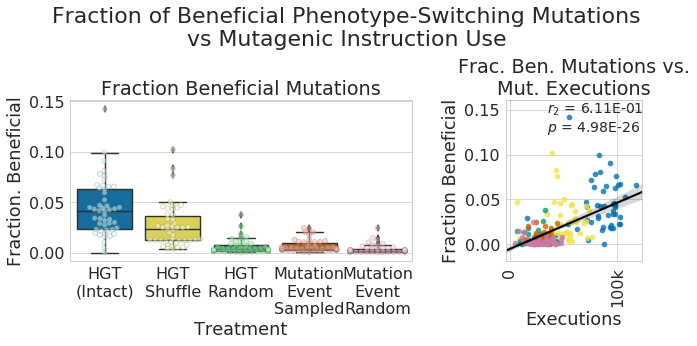
\includegraphics[width=0.7\columnwidth]{figures/HGT/mutagen_use_vs_fraction_beneficial.png}
\caption{bleh
}\label{fig:mutagen_use_vs_fraction_beneficial}
\end{center}
\end{figure}

%HGT conveys greater proportions of beneficial phenotype-changing mutations than other mutagens.


\section{Conclusion}
%CE selects for evolvability 
%* Because HGT is much more beneficial than other types of mutation
%Under Stress, Natural Competence increases
Our experiments expand on our understanding of the evolution of horizontal gene transfer, and how it relates to other types of mutations in the context of changing environments. As expected, we find that the fitness effects of different types of mutations vary significantly, and that they predict the levels of use of that mutagen. In particular, we find a strong correlation between the fraction of mutations that produce a beneficial phenotype change, and the use of that mutagen. Thus, in the context of a changing environment, where there are strong selective pressures to change your phenotype, levels of HGT are elevated, while levels of other mutagens remain low.

This result matches prior research that shows that populations will tend to depress the use of mutagens, even though, in the long-term, higher mutation rates are optimal [CITE]. This result is further evidence that selection tends to act in the short term. Thus, even though certain kinds of mutagens and architectural features may promote long-term evolvability, these features are hitchhiking on short-term adaptive benefits. Thus, our research shows that even though evolvability may evolve, it is not necessarily selected for in the long-term. 

\todo{add a takeaway, as per the note below}
% MJW: Since this is a conclusion section, it's worth taking a bit of space to drive home the major points, even if this seems a bit repetitive with the discussion section.  If I'm remembering the results correctly: Simply boosting the mutation rate doesn't cause the instruction to be notably enriched.  That means that the higher effective mutation rate caused by these HGT events is not what's driving things.  Causing that number of mutations to all localize to one region does cause the instruction's use to be elevated, so there's some advantage to this localization.  But there's a *much* higher use if there is also information content involved, either by enriching for those instructions in the actual fragment, or even moreso if the order of those instructions is preserved.  This means that primary beneficial effect of HGT we see is that it results in mutation events that contain more information content than other types of mutation events.

\todo{does this (below) read ok?}
As in the experiments described in the previous chapter, performing these kinds of experiments in an organic system would be extremely difficult. In particular, comparing the effects of different kinds of mutations, measuring their use, and isolating their fitness effects would be extremely difficult or even impossible. Digital evolution allows us to perform these kinds of experiments that otherwise could not be done in natural systems. 
% MJW: And, like in the previous chapter, either in this conclusion or at the end of the Discussion, and almost certainly in the Background section, you can hammer home "Yay digital evolution" by pointing out how unbelievably difficult this work would be in a physical system.
%@RCK: Added something. Someone please read over!

%%%%%%%%%%%%%%%%%%%%%%%%%%%%%%%%%%%%%%%%%%%%%%%%%%%%%%%%%%%%%%%%%%%%%%%%%%%%%%%%%%%%%%%%%%%%%%
%%%%%%%%%%%%%%%%%%%%%%%%%%%%%%%%%%%%%%%%%% CHAPTER 5 %%%%%%%%%%%%%%%%%%%%%%%%%%%%%%%%%%%%%%%%%
%%%%%%%%%%%%%%%%%%%%%%%%%%%%%%%%%%%%%%%%%%%%%%%%%%%%%%%%%%%%%%%%%%%%%%%%%%%%%%%%%%%%%%%%%%%%%%



\chapter{Changing Environments and Long Term Evolvability}
\label{chap:ce-longterm}
\section{Background}

%=how it affects long-term evo
For longer timescales, evolvability is concerned more with variability generation and exploration of neutral spaces. Populations that exhibit this kind of evolvability would possess genomes with genetic architectures that more easily traverse the mutational landscape along neutral roads and thereby discover new fitness peaks while avoiding crossing fitness valleys. This kind of evolvability would allow populations to more easily colonize new ecological niches and form new clades\cite{kirschner_evolvability_1998,brookfield_evolution:_2001}.

%=connection between short/long term evo non-obvious
Despite some common features, the relationship between short-term and long-term evolvability is not obvious. Architectural features and evolutionary pressures that might convey short-term evolvability may not be the same as those that confer longer-term evolvability\cite{pigliucci_is_2008}. For example, features that promote rapid adaptation to a harsh fluctuating environment might reduce fitness in constant or benign fluctuating environments as compared to that of wild-type invaders. Alternately, the adaptation to harsh fluctuating environments and the resulting bottlenecks would potentially reduce diversity to the point where large amounts of neutral novelty generation could not occur.

\todo[color=magenta,inline]{ch5 - background - fill this in about the prior research done in this area}
Prior research has shown that...

In this chapter, we examine how changing environments or novel mutagens affect long-term evolutionary potential. We introduce change-evolved populations from prior experiments with changing environments, and the evolution of HGT, to an entirely new environment, where we can assess long-term variability generation in the form of new task discovery and exploration.

\section{Methods}
% For most experiments described in this chapter, we use populations of Avida organisms that were originally evolved in other experimental treatments with changing environments. We use populations evolved in Chapter~\ref{chap:ce-adaptation} to survey long-term evolutionary potential that originate in simple changing environments with a single fluctuating task. We use populations evolved in Chapter~\ref{chap:evo-hgt}, in a more complex changing environment, with the presence of the HGT instruction, evolved both with and without a bonus. And finally, we evolve a new set of populations that originate in a complex changing environment, but without exposure to HGT. 

\subsection{Experimental Design}
%=design for experimental environment (CCE vs SCE, and short vs long)
In order to examine the long-term dynamics and mechanisms of evolving populations in changing environments, we performed three sets of experiments. For each set of experiments, we take populations evolved in conditions where short-term evolvability pressures dominate, and we introduce the resulting populations to a completely new environment, with a new set of rewarded bitwise tasks to perform: Logic-77. These new tasks use three bitwise inputs rather than two, and are each rewarded with a constant 1.2-fold bonus to execution. This reward structure provides a mild selective pressure to evolve these task, but the benefits to performing them do not overwhelm the existing selective pressure to continue performing the tasks rewarded by the original changing or static environment. 

The first set of experiments examines the dynamics of organisms that originally evolved in simple changing environments. These are a continuation of the experiments described in Chapter~\ref{chap:ce-adaptation}. The second set of experiments takes populations evolved in a more complex changing environment where we evolve the organisms to switch back and forth between two halves of the Logic-9 task set. For the final set of experiments, we take populations that evolved in a complex changing environment, similar to the second set, but with the addition of the HGT mutagen. These are a continuation of experiments described in Chapter~\ref{chap:evo-hgt}.

With these experiments, we will explore the characteristics of these populations, and how different kinds of environmental conditions do or do not produce long-term evolvability.  

\subsubsection{Simple Cyclic Changing Environments}
%=explanation of the changing environment treatments - cyclic
We took populations evolved under the experimental conditions detailed in Chapter \ref{chap:ce-adaptation}, and introduced them to an entirely new set of rewarded bitwise logical tasks: the Logic-77 environment. 

\todo[inline, color=magenta]{CH5 methods - more details about each treatment}

	%=[TABLE - experimental treatments]
	\begin{table}[]
	\centering
	\caption{\textbf{Experimental Treatments - Simple Cyclic Changing Environment}}
	\label{cel-treatments-h}

	\begin{tabular}{|c|c||c|c||c|c|c|}
	%\begin{tabular}{ccccccc}
	\hline
	\multirow{3}{*}{ \thead{Treatment} } & \multirow{3}{*}{ \thead{Changing \\ Env. \\ Type} } & \multicolumn{5}{c|}{ \thead{Rewarded Tasks} } \\\cline{3-7}
	& & \multicolumn{2}{c||}{ \thead{Phase 1 \\ (0-200,000 Updates)} } & \multicolumn{3}{c|}{ \thead{Phase 2 \\ (200,000-400,000 Updates)} } \\\cline{3-7}
	& & XOR & EQU & XOR & EQU & \makecell{Logic-77 \\ (all)} \\\hhline{|=|=|=|=|=|=|=|}
	Control & \makecell{None \\ (static)} & \makecell{constant \\ $2^3$} & \makecell{constant \\ $2^5$} & \makecell{constant \\ $2^3$} & \makecell{constant \\ $2^5$} & \makecell{constant \\ $2^{0.3}$} \\\hline
	Benign & Cyclic & \makecell{constant \\ $2^3$} & \makecell{benign \\ fluctuating \\ 0 or $2^5$} & \makecell{constant \\ $2^3$} & \makecell{benign \\ fluctuating \\ 0 or $2^5$} & \makecell{constant \\ $2^{0.3}$} \\\hline
	\makecell{Benign \\ Quiesce} & Cyclic & \makecell{constant \\ $2^3$} & \makecell{benign \\ fluctuating \\ 0 or $2^5$} & \makecell{constant \\ $2^3$} & \makecell{constant \\ $2^5$} & \makecell{constant \\ $2^{0.3}$} \\\hline
	Harsh & Cyclic & \makecell{constant \\ $2^3$} & \makecell{harsh \\ fluctuating \\ $-2^5$ or $2^5$} & \makecell{constant \\ $2^3$} & \makecell{harsh \\ fluctuating \\ $-2^5$ or $2^5$} & \makecell{constant \\ $2^{0.3}$} \\\hline
	\makecell{Harsh \\ Quiesce} & Cyclic & \makecell{constant \\ $2^3$} & \makecell{harsh \\ fluctuating \\ $-2^5$ or $2^5$} & \makecell{constant \\ $2^3$} & \makecell{constant \\ $2^5$} & \makecell{constant \\ $2^{0.3}$} \\\hline
	%\makecell{Harsh \\ to \\ Benign} & Cyclic & \makecell{constant \\ $2^3$} & \makecell{harsh \\ fluctuating \\ $-2^5$ or $2^5$} & \makecell{constant \\ $2^3$} & \makecell{benign \\ fluctuating \\ 0 or $2^5$} & \makecell{constant \\ $2^{0.3}$} \\\hline
	\end{tabular} 

	\begin{flushleft} Experimental treatments. Four types of cyclic changing environment, plus a static control. Each is split into two phases. The first phase is a normal changing environment like those found in Chapter~\ref{chap:ce-adaptation}, Table~\ref{ce-treatments-h}. The second phase introduces an additional set of tasks (Logic 77) that are rewarded at a lower rate.
	\end{flushleft}
	\label{cel-treatments}
	\end{table}


%=the organisms
As in Chapter \ref{chap:ce-adaptation}, we held the individual genomes at a fixed length of 121 instructions, and applied mutations after each successful replication event at a substitution probability of 0.00075 per site. Again, we configured the Avida world to have local interactions on a toroidal grid that is 60-by-60 cells (3600 cells in total), and continued the evolution of populations where we left off in Chapter~\ref{chap:ce-adaptation}.

\subsubsection{Complex Cyclic Changing Environment}
The second set of experiments looks at the evolution of populations of organisms with variable-length genomes, evolved in a more complex cyclic changing environment. This environment and genetic structure derives from the experiments described in \ref{chap:evo-hgt}. However, these populations were evolved without a working HGT instruction.

\todo{update table to match HGT}
	%=[TABLE - experimental treatments]
	\begin{table}[]
	\centering
	\caption{\textbf{Experimental Treatments - Complex Cyclic Changing Environment}}
	\label{cel-treatments-h}

	\begin{tabular}{|c|c||c|c||c|c|c|}
	%\begin{tabular}{ccccccc}
	\hline
	\multirow{3}{*}{ \thead{Treatment} } & \multirow{3}{*}{ \thead{Changing \\ Env. \\ Type} } & \multicolumn{5}{c|}{ \thead{Rewarded Tasks} } \\\cline{3-7}
	& & \multicolumn{2}{c||}{ \thead{Phase 1 \\ (0-200,000 Updates)} } & \multicolumn{3}{c|}{ \thead{Phase 2 \\ (200,000-400,000 Updates)} } \\\cline{3-7}
	& & XOR & EQU & XOR & EQU & \makecell{Logic-77 \\ (all)} \\\hhline{|=|=|=|=|=|=|=|}
	Control & \makecell{None \\ (static)} & \makecell{constant \\ $2^3$} & \makecell{constant \\ $2^5$} & \makecell{constant \\ $2^3$} & \makecell{constant \\ $2^5$} & \makecell{constant \\ $2^{0.3}$} \\\hline
	Benign & Cyclic & \makecell{constant \\ $2^3$} & \makecell{benign \\ fluctuating \\ 0 or $2^5$} & \makecell{constant \\ $2^3$} & \makecell{benign \\ fluctuating \\ 0 or $2^5$} & \makecell{constant \\ $2^{0.3}$} \\\hline
	\makecell{Benign \\ Quiesce} & Cyclic & \makecell{constant \\ $2^3$} & \makecell{benign \\ fluctuating \\ 0 or $2^5$} & \makecell{constant \\ $2^3$} & \makecell{constant \\ $2^5$} & \makecell{constant \\ $2^{0.3}$} \\\hline
	Harsh & Cyclic & \makecell{constant \\ $2^3$} & \makecell{harsh \\ fluctuating \\ $-2^5$ or $2^5$} & \makecell{constant \\ $2^3$} & \makecell{harsh \\ fluctuating \\ $-2^5$ or $2^5$} & \makecell{constant \\ $2^{0.3}$} \\\hline
	\makecell{Harsh \\ Quiesce} & Cyclic & \makecell{constant \\ $2^3$} & \makecell{harsh \\ fluctuating \\ $-2^5$ or $2^5$} & \makecell{constant \\ $2^3$} & \makecell{constant \\ $2^5$} & \makecell{constant \\ $2^{0.3}$} \\\hline
	%\makecell{Harsh \\ to \\ Benign} & Cyclic & \makecell{constant \\ $2^3$} & \makecell{harsh \\ fluctuating \\ $-2^5$ or $2^5$} & \makecell{constant \\ $2^3$} & \makecell{benign \\ fluctuating \\ 0 or $2^5$} & \makecell{constant \\ $2^{0.3}$} \\\hline
	\end{tabular} 

	\begin{flushleft} Experimental treatments. Four types of cyclic changing environment, plus a static control. Each is split into two phases. The first phase is a normal changing environment similar to those found in Chapter~\ref{chap:ce-adaptation}, Table~\ref{ce-treatments-h}. The second phase introduces an additional set of tasks (Logic 77) that are rewarded at a lower rate.
	\end{flushleft}
	\label{cel-treatments}
	\end{table}

\todo[color=magenta,inline]{TODO fill this in with more detail of each treatment}

\subsubsection{Complex Cyclic Changing Environment with HGT mutagen}
The last set of experiments looks at the evolution of populations of organisms that evolved in a more complex cyclic changing environment, while having access to the HGT mutagen. These experiments are continuations of those described in \ref{chap:evo-hgt}, and continue the evolution of the populations evolved there.

%=[TABLE - experimental treatments]
\begin{table}[]
\centering
\caption{\textbf{Experimental Treatments - Complex Cyclic Changing Environments with HGT}}
\label{cel-treatments-h}
\todo[color=red, inline]{correct second half of the table with info about the bonus structures B0 and B0.8}
	\begin{tabular}{|c|c||c|c||c|c|c|}
	%\begin{tabular}{ccccccc}
	\hline
	\multirow{3}{*}{ \thead{Treatment} } & \multirow{3}{*}{ \thead{Changing \\ Env. \\ Type} } & \multicolumn{5}{c|}{ \thead{Rewarded Tasks} } \\\cline{3-7}
	& & \multicolumn{2}{c||}{ \thead{Phase 1 \\ (0-200,000 Updates)} } & \multicolumn{3}{c|}{ \thead{Phase 2 \\ (200,000-400,000 Updates)} } \\\cline{3-7}
	& & XOR & EQU & XOR & EQU & \makecell{Logic-77 \\ (all)} \\\hhline{|=|=|=|=|=|=|=|}
	Control & \makecell{None \\ (static)} & \makecell{constant \\ $2^3$} & \makecell{constant \\ $2^5$} & \makecell{constant \\ $2^3$} & \makecell{constant \\ $2^5$} & \makecell{constant \\ $2^{0.3}$} \\\hline
	Benign & Cyclic & \makecell{constant \\ $2^3$} & \makecell{benign \\ fluctuating \\ 0 or $2^5$} & \makecell{constant \\ $2^3$} & \makecell{benign \\ fluctuating \\ 0 or $2^5$} & \makecell{constant \\ $2^{0.3}$} \\\hline
	\makecell{Benign \\ Quiesce} & Cyclic & \makecell{constant \\ $2^3$} & \makecell{benign \\ fluctuating \\ 0 or $2^5$} & \makecell{constant \\ $2^3$} & \makecell{constant \\ $2^5$} & \makecell{constant \\ $2^{0.3}$} \\\hline
	Harsh & Cyclic & \makecell{constant \\ $2^3$} & \makecell{harsh \\ fluctuating \\ $-2^5$ or $2^5$} & \makecell{constant \\ $2^3$} & \makecell{harsh \\ fluctuating \\ $-2^5$ or $2^5$} & \makecell{constant \\ $2^{0.3}$} \\\hline
	\makecell{Harsh \\ Quiesce} & Cyclic & \makecell{constant \\ $2^3$} & \makecell{harsh \\ fluctuating \\ $-2^5$ or $2^5$} & \makecell{constant \\ $2^3$} & \makecell{constant \\ $2^5$} & \makecell{constant \\ $2^{0.3}$} \\\hline

	Control & \makecell{None \\ (static)} & \makecell{constant \\ $2^3$} & \makecell{constant \\ $2^5$} & \makecell{constant \\ $2^3$} & \makecell{constant \\ $2^5$} & \makecell{constant \\ $2^{0.3}$} \\\hline
	Benign & Cyclic & \makecell{constant \\ $2^3$} & \makecell{benign \\ fluctuating \\ 0 or $2^5$} & \makecell{constant \\ $2^3$} & \makecell{benign \\ fluctuating \\ 0 or $2^5$} & \makecell{constant \\ $2^{0.3}$} \\\hline
	\makecell{Benign \\ Quiesce} & Cyclic & \makecell{constant \\ $2^3$} & \makecell{benign \\ fluctuating \\ 0 or $2^5$} & \makecell{constant \\ $2^3$} & \makecell{constant \\ $2^5$} & \makecell{constant \\ $2^{0.3}$} \\\hline
	Harsh & Cyclic & \makecell{constant \\ $2^3$} & \makecell{harsh \\ fluctuating \\ $-2^5$ or $2^5$} & \makecell{constant \\ $2^3$} & \makecell{harsh \\ fluctuating \\ $-2^5$ or $2^5$} & \makecell{constant \\ $2^{0.3}$} \\\hline
	\makecell{Harsh \\ Quiesce} & Cyclic & \makecell{constant \\ $2^3$} & \makecell{harsh \\ fluctuating \\ $-2^5$ or $2^5$} & \makecell{constant \\ $2^3$} & \makecell{constant \\ $2^5$} & \makecell{constant \\ $2^{0.3}$} \\\hline

	\end{tabular} 

	\begin{flushleft} Experimental treatments. Four types of cyclic changing environment, plus a static control. Each is split into two phases. The first phase is a normal changing environment similar to those found in Chapter~\ref{chap:ce-adaptation}, Table~\ref{ce-treatments-h}. The second phase introduces an additional set of tasks (Logic 77) that are rewarded at a lower rate.
	\end{flushleft}
	\label{cel-treatments}
	\end{table}

\todo[color=magenta,inline]{TODO fill this in with more detail of each treatment}

\subsection{Measuring Task Discovery and Task Performance}
In order to assess how populations adapt to a brand new environment, we measure Task Performance and Task Discovery.

\subsubsection{Task Performance}
Task Performance is measured by counting the number of unique non-ephemeral tasks that a population is performing. Each task may be performed only once per organism, yielding a maximum task count of 3600 at any given time. Thus, we define a non-ephemeral task as one that a population is performing at equal to or more than 0.1\% level, or 3.6 times per sampling. 

\subsubsection{Task Discovery}
We measure task by counting the number of unique non-ephemeral tasks that have been discovered by a population, starting at a defined point in time. Once a task is discovered, it may not become "undiscovered." Thus, task discovery counts will always increase monotonically. We measure "Overall" task discovery, counting all possible tasks - including Logic-77 which were available, but not rewarded in the first phase of experiments - and also "Post-Reward" task discovery, where we begin counting new tasks from the beginning of the second phase of the experiment, once Logic-77 rewards are applied. 

\section{Results and Discussion}

Our experiments demonstrate that the harshness of fluctuation has a dramatic effect on long-term evolvability, landscape exploration and task discovery. We find that while harsh changing environments were most effective at driving short-term adaptation, these environments depress long-term evolvability once rewards are in place. In all experiments, we find that benign environments produce the highest levels of task discovery, far outperforming harsh changing environments. We also find that the HGT mutagen, which helps with short-term evolvability in cyclic environments, does not appear to have a beneficial effect.

\subsection{Long-Term Evolvability in Simple Cyclic Changing Environments}

\subsubsection{Benign changing environments outperform harsh environments in task discovery}
We found that once the Logic-77 reward structure is introduced, populations evolving in harsh changing environments discover many fewer tasks that those evolving in benign changing environments (Fig~\ref{fig:postreward_task_discovery})\todo{stats}. We hypothesize that this effect is due to the relative differences in the strength of selection between the harsh changing environment and the directional selection toward the logic-77 tasks. The pressure to gain and lose the fluctuating task is much stronger than the pressure to acquire the logic-77 tasks, thereby depressing the rate at which they are found.
%and keeping it comparable to the pre-phase 2 rate. 
In contrast, the benign environment, with its comparatively weaker strength of selection for EQU task gain and loss, experiences a comparatively stronger selective pressure to acquire logic-77 tasks, while still benefiting from the increased exploration rate conveyed by the benign changing environment.

	%=[FIGURE - postreward task discovery]
	\todo[color=green]{stats}
	\todo{caption}
	\begin{figure}[!h]
	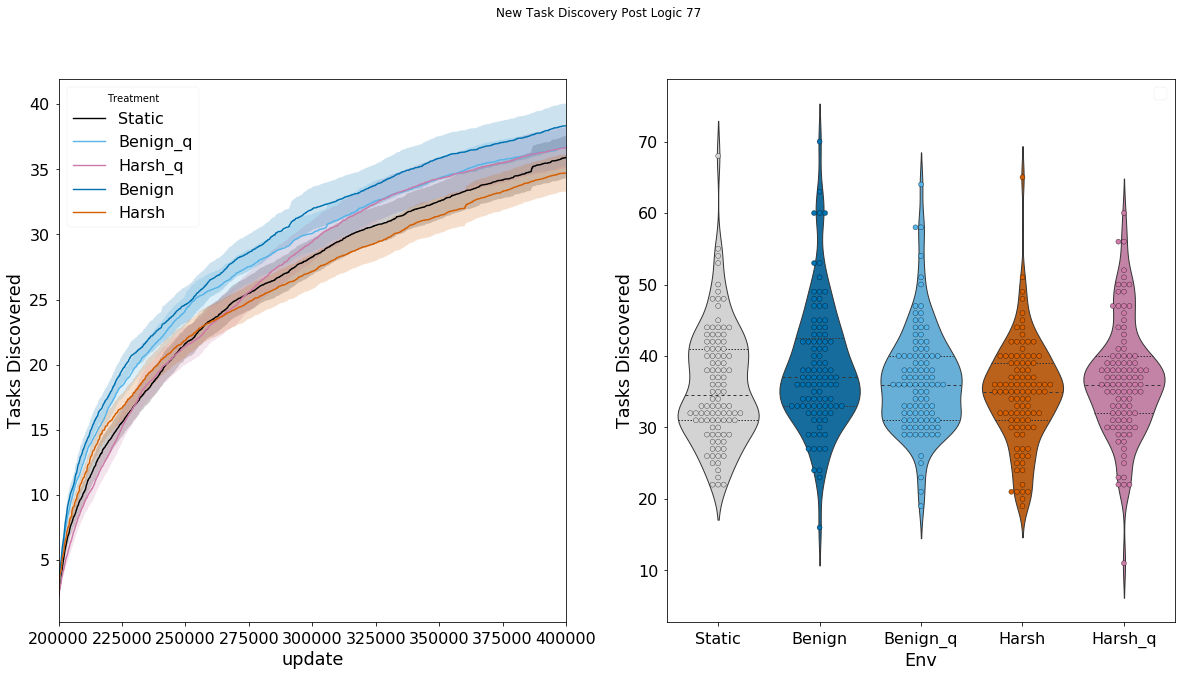
\includegraphics[trim={0 0 0 0}, clip, width=0.75\columnwidth]{figures/LTE/lte-simple-post_reward_task_discovery.png}
	\caption{\textbf{Number of new logic-77 tasks discovered beginning in phase 2}.%
	}
	\label{fig:postreward_task_discovery}
	\end{figure} 

Interestingly, in those populations where we removed the harsh environmental change as we introduce Logic-77, we see that task exploration recovers somewhat and reaches a comparable level to the control\todo{stats}. This suggests that it is the active pressures of the harsh environment that depress task exploration, and not a penalty conveyed by architectural features that persist after selective pressures have changed.

%=disentangling direct effects from architectural byproducts
Of similar interest is the comparison of task discovery rates between the benign changing environment populations BenignCE and BenignQuiescent.\todo{make a figure to highlight this?}\todo{rename the populations A and B} The BenignCE populations continue to be subject to the benign changing environment, where as the BenignQuiescent populations are only subject to directional selection toward the evolution of XOR, EQU, and the Logic-77 tasks. The task discovery rate for the BenignCE population is slightly higher than for BenignQuiescent, but the effect is not statistically significant\todo{stats}. Both, however, still perform better than the control treatment\todo{stats}. Thus, this result suggests that there may be architectural features conferred by evolution in the changing environment that are helpful for long-term evolvability, even after the environmental changes have stopped, and that this effect is distinct from the direct effects of the changing direction of selection. %Further research is needed to fully untangle these effects.

 

\subsubsection{Benign changing environments outperform harsh environments in task performance}
Similar to task discovery, populations evolving in harsh changing environments perform far fewer distinct tasks than either the benign-evolved or control populations (Fig~\ref{fig:lte-task_performance})\todo{stats}. While the Benign-evolving populations seem to outperform the control, this effect is not statistically significant.\todo{stats} 

	%=[FIGURE - postreward task performance]
	\todo[color=green]{stats}
	\todo{caption}
	\begin{figure}[!h]
	%\missingfigure{lte-task_performance - Long Term Evolution Task Performance}
	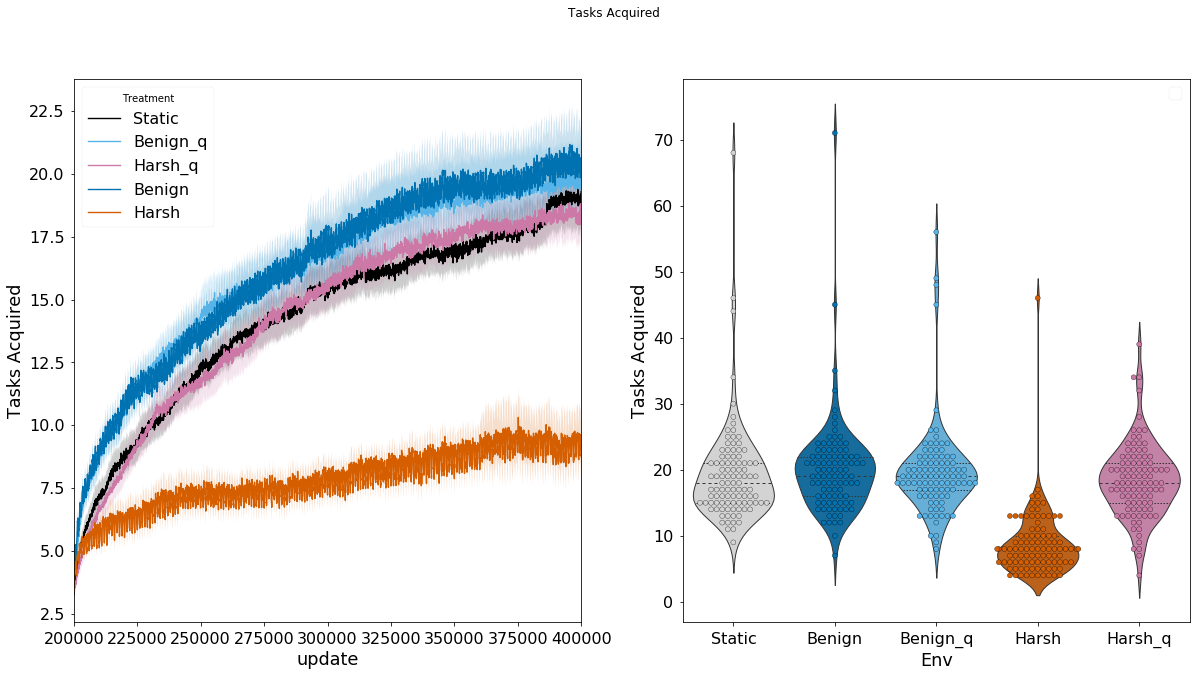
\includegraphics[trim={0 0 0 0}, clip, width=0.75\columnwidth]{figures/LTE/lte-simple-post_reward_task_performance.png}
	%\missingfigure{Long Term Evolution Task Performance}
	\caption{\textbf{Number of new logic-77 tasks performed beginning in phase 2}.%
	}
	\label{fig:lte-task_performance}
	\end{figure}  


\subsubsection{Harsh changing environments drive populations across the mutational landscape}
%=choice of CE has dramatic effects - forced march
In the first phase of the experiments, despite the logic-77 tasks not being rewarded, both changing-environment treatments discover more new tasks than the control\todo{stats}. The harsh changing environment treatments in particular discover significantly more Logic-77 tasks than either the benign treatment\todo{stats}, or the control, despite these tasks not being rewarded (Fig~\ref{fig:overall_task_discovery}. We hypothesize that this effect may be due to the large phylogenetic depth of the harsh-evolved populations, where the repeated bottlenecks drive the populations along a kind of forced march across the mutational landscape. However, as the experiment proceeds, and Logic-77 rewards are introduced, this effect disappears, and benign environments quickly dominate in task discovery.\todo{stats}

%=[FIGURE - overall task discovery]
\todo[inline]{REPLACE THIS WITH THE ONE THAT HAS THE VIOLIN PLOT?}
\todo[color=green]{stats}
\todo{caption}
	\begin{figure}[!h]
	\includegraphics[trim={0 0 0 0}, clip, width=0.75\columnwidth]{figures/LTE/901_overall_task_discovery.png}
	\caption{\textbf{Number of new logic-77 tasks discovered over time}. [TODO DESCRIPTION AND STATS]%
	}
	\label{fig:overall_task_discovery}
	\end{figure}

%=post-reward exploration - strength of selection differences
% Despite the initial success of the harsh-evolved populations' random walk across the fitness landscape, once selection for the logic-77 tasks is engaged at the start of phase 2, the benign and control treatments out-perform the harsh-evolved populations in task discovery. In particular, those populations where the harsh changing environment continues, significantly under-perform in task exploration as compared to the benign-evolved populations, and are comparable to the control rate. (Fig~\ref{fig:postreward_task_discovery}). 
% (Fig~\ref{fig:composite_task_discovery} lower left)







% %=[FIGURE - overall task discovery]
% \todo[color=green]{stats}
% \todo{caption}
% \begin{figure}[!h]
% 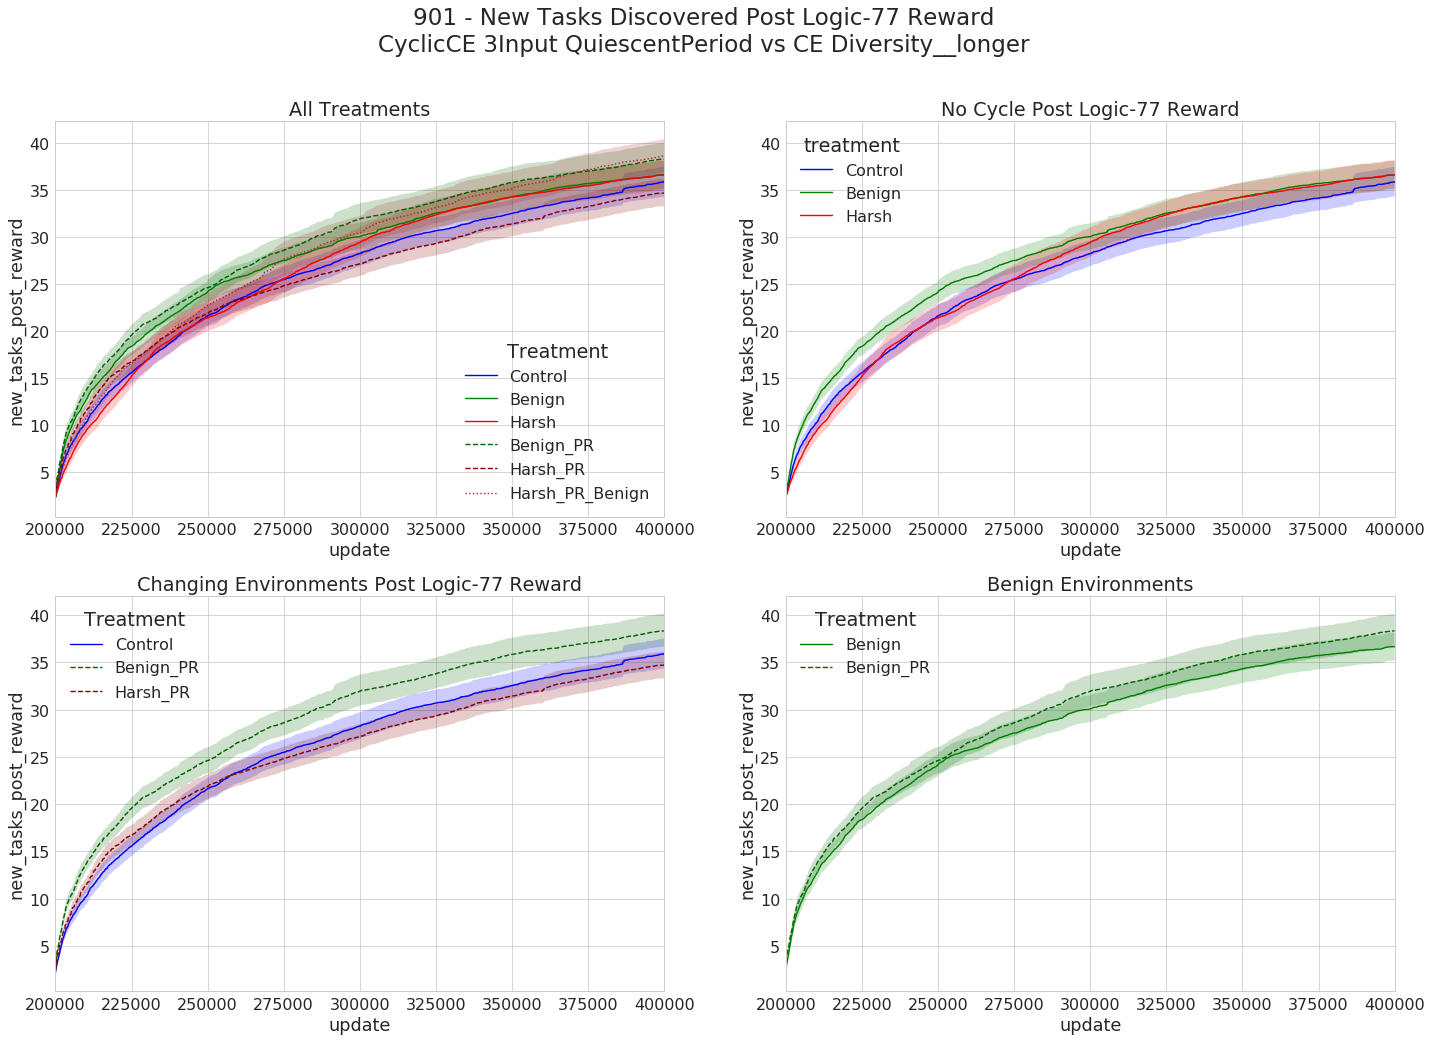
\includegraphics[trim={0 0 0 0}, clip, width=1\columnwidth]{figures/CE/901_postreward_composites_task_discovery.png}
% \caption{\textbf{Detail of task discovery rates over time}. %
% }
% \label{fig:composite_task_discovery}
% \end{figure}

\subsection{Long Term Evolvability and Complex Changing Environments}

\subsubsection{Benign changing environments outperform harsh environments in task discovery and task performance}
Similar to the results of the simple environments, Benign-evolved populations out-perform Harsh-evolving populations in complex changing environments in measures of Task Performance (Fig~\ref{fig:complex-task_performance}) and Task Discovery (Fig~\ref{fig:complex-task_discovery}). Again, this result suggests that, despite the differences in genome composition and environmental complexity, Benign changing environments, with their gentler selective pressures, or possibly with more intact chunks of undisturbed functionality in their genomes, leave more room for populations to acquire new tasks without the risk of harsh punishments. 
%MAYBE NOT?
%Both types of Benign-evolved environment appear to out-perform the control, but the effect is not statistically significant.

%=[FIGURE - complex environment task performance]
\todo[color=green]{stats}
\todo{caption}
	\begin{figure}[!h]
	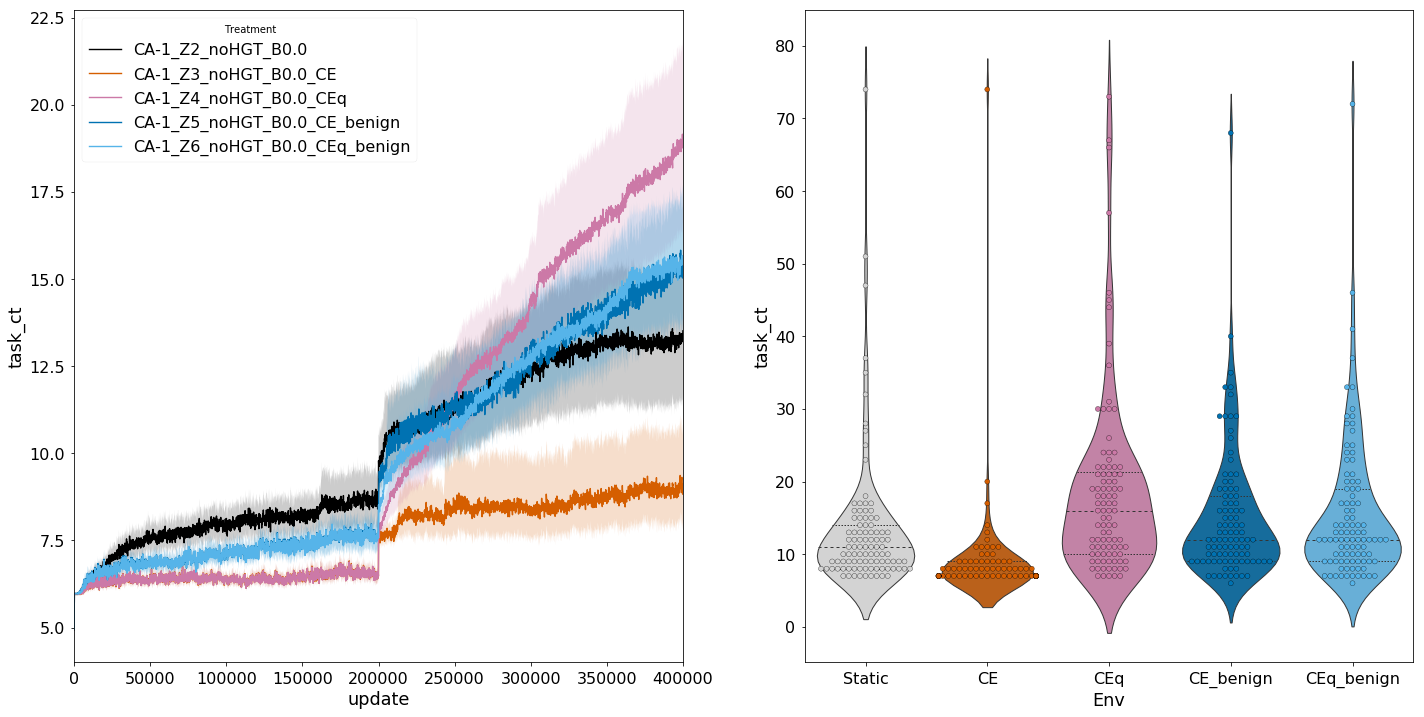
\includegraphics[trim={0 0 0 0}, clip, width=0.75\columnwidth]{figures/LTE/lte-complex-task_performance.png}
	%\missingfigure{Complex CCE Task Performance}
	\caption{\textbf{Number of logic-77 tasks performed over time}. [TODO DESCRIPTION AND STATS]%
	}
	\label{fig:complex-task_performance}
	\end{figure}

%=[FIGURE - complex environment task discovery]
\todo[color=green]{stats}
\todo{caption}
	\begin{figure}[!h]
	%\missingfigure{Complex CCE Task Discovery}
	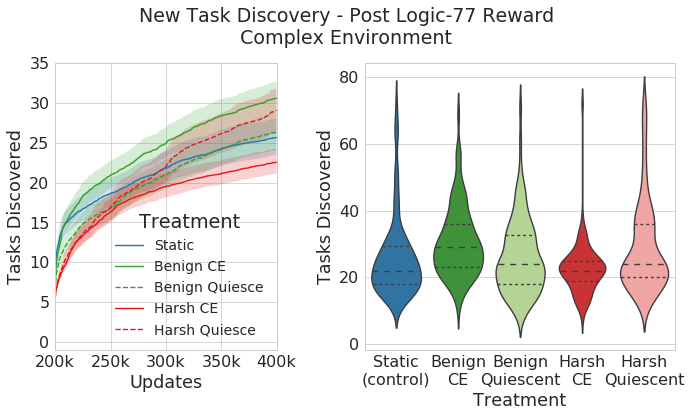
\includegraphics[trim={0 0 0 0}, clip, width=0.75\columnwidth]{figures/LTE/lte-complex-post_reward_task_discovery.png}
	\caption{\textbf{Number of new logic-77 tasks discovered post-reward}. [TODO DESCRIPTION AND STATS]%
	}
	\label{fig:complex-task_discovery}
	\end{figure}

% below is speculative!!!
Interestingly, populations that were initially evolved in a harsh changing environment and then change ceased upon introduction of Logic-77 rewards (HarshQuiescent) seem to out-perform all other environment types in task performance (Fig~\ref{fig:complex-task_performance}) \todo{stats}. This effect may be due to a lingering architectural effect of evolving in harsh changing environments. Further research is needed to identify a mechanism for this effect.



\subsection{Long Term Evolvability and Horizontal Gene Transfer}
\todo{move below to the introduction about why we care about HGT}
The addition of mutagens are thought to promote long-term evolvability[CITE] In this section we examine the long-term evolutionary dynamics of adding an HGT mutagen to populations introduced to a brand new, complex environment.

\subsubsection{New environments do not promote the use of HGT}
Contrary to our expectations, none of our populations previously evolved to use HGT showed a significant increase in HGT fragment uptakes as a result of being introduced to a new environment\todo{stats}. In general, levels remain constant, and in one notable example, levels appear to decrease, though this effect is not statistically significant (Fig ~\ref{fig:lte-hgt_use}.

%=[FIGURE - complex environment task discovery]
\todo[color=green]{stats}
\todo{caption}
	\begin{figure}[!h]
	\missingfigure{HGT Use Bonus 0, split by pre and post introduction of new logic-77 tasks}
	%\includegraphics[trim={0 0 0 0}, clip, width=0.75\columnwidth]{figures/CE/901_overall_task_discovery.png}
	\caption{\textbf{HGT Use, pre and post introduction of new logic-77 tasks}. [TODO DESCRIPTION AND STATS]%
	}
	\label{fig:lte-hgt_use}
	\end{figure}

\subsubsection{Fragment grazing bonus reduces task discovery and task performance}
In most of our environmental treatments, applying an HGT Uptake grazing bonus results in reduced levels of both task performance and task discovery\todo{stats} as compared to non-Bonus treatments (Fig~\ref{fig:lte-hgt_task_performance}, and Fig~\ref{fig:lte-hgt_task_discovery}).
\todo{hypothesis here?}
%We hypothesize that this reduction may occur because populations may already be adapted and resistant to performing HGT, and thus, performing it is an easy way to increase fitness. 

%=[FIGURE - complex environment task discovery]
\todo[color=green]{stats}
\todo{caption}
	\begin{figure}[!h]
	%\missingfigure{HGT Use}
	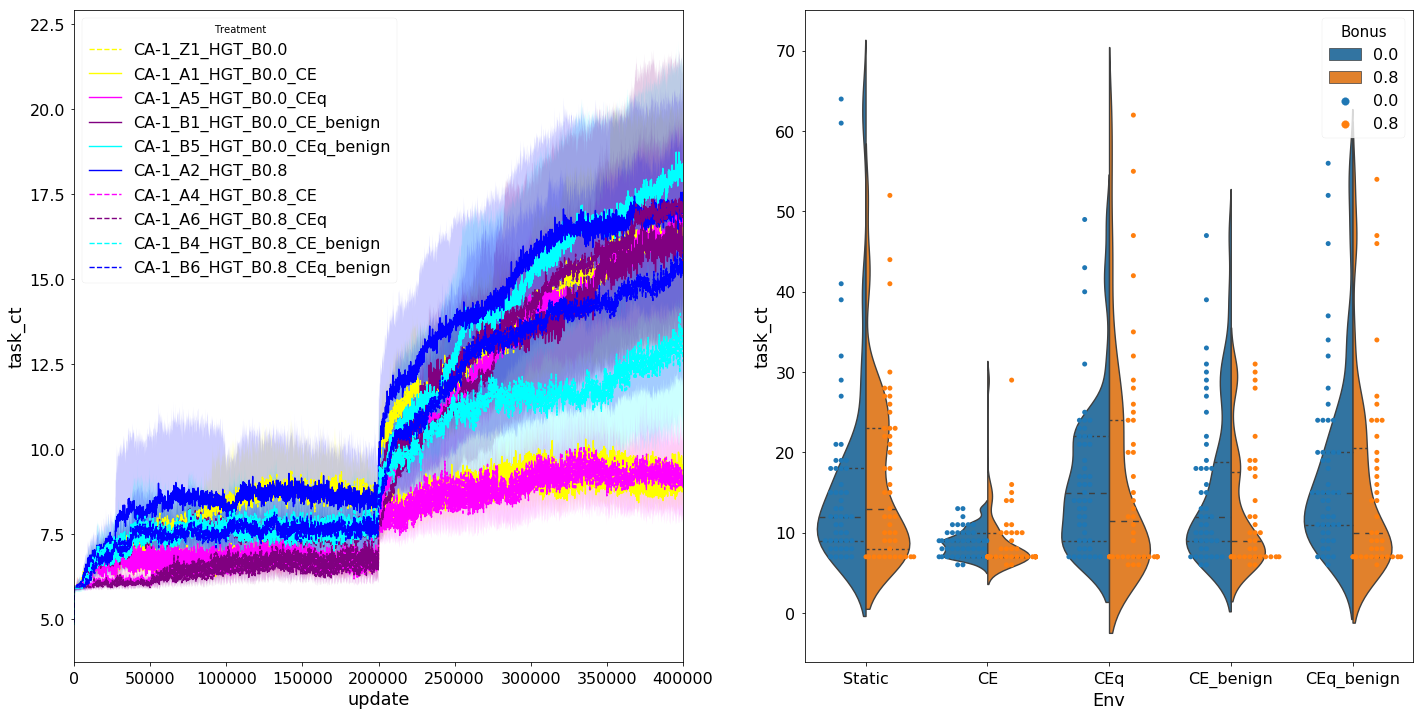
\includegraphics[trim={0 0 0 0}, clip, width=0.75\columnwidth]{figures/LTE/lte-hgt-task_performance.png}
	\caption{\textbf{Task Performance, with and without HGT Grazing Bonus}. [TODO DESCRIPTION AND STATS]%
	}
	\label{fig:lte-hgt_task_performance}
	\end{figure}

%=[FIGURE - complex environment task discovery]
\todo[color=green]{stats}
\todo{caption}
	\begin{figure}[!h]
	%\missingfigure{HGT Use}
	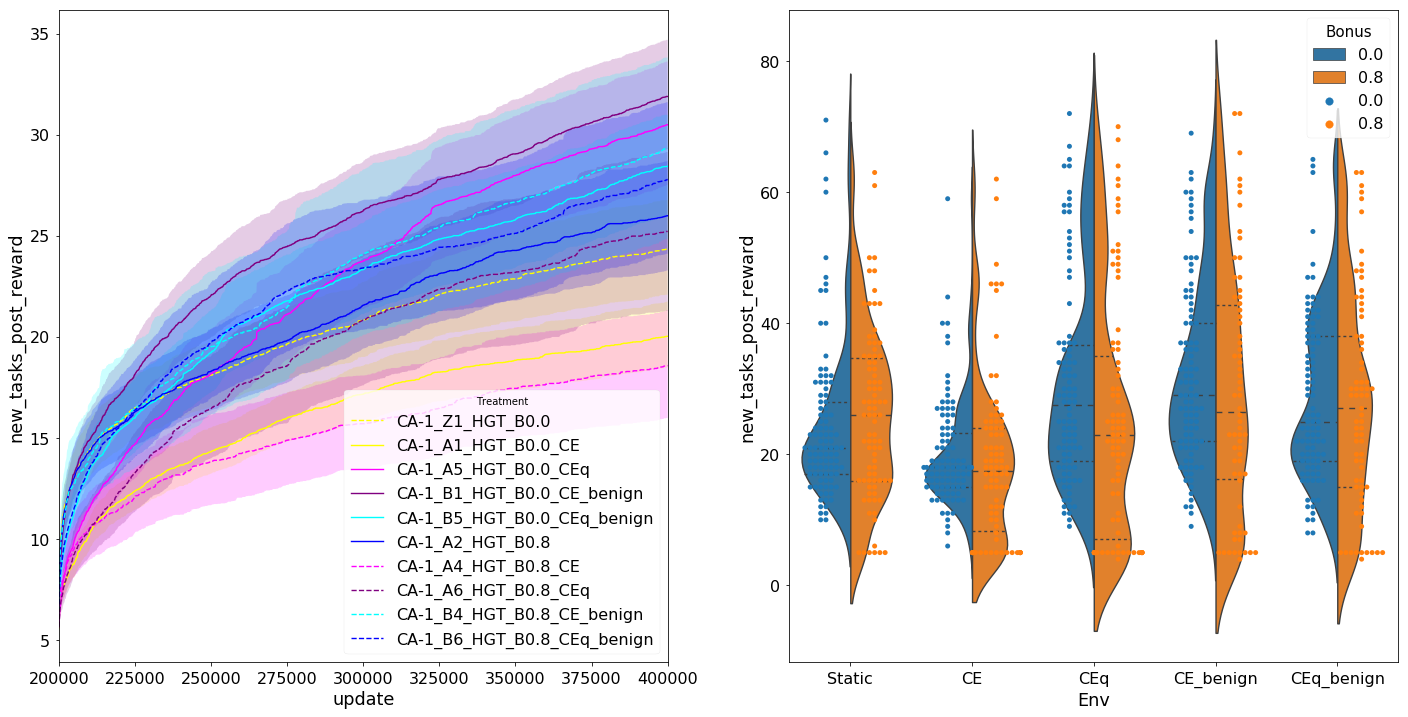
\includegraphics[trim={0 0 0 0}, clip, width=0.75\columnwidth]{figures/LTE/lte-hgt-task_discovery.png}
	\caption{\textbf{Task Discovery, with and without HGT Grazing Bonus}. [TODO DESCRIPTION AND STATS]%
	}
	\label{fig:lte-hgt_task_discovery}
	\end{figure}

Further, we see a strong negative correlation between task discovery and task performance in populations where an HGT grazing bonus is applied, regardless of environmental treatment (Fig~\ref{fig:lte-bonus_hgt_vs_task_performance}. We see no such correlation in non-Bonus HGT populations (Fig~\ref{fig:lte-no-bonus_hgt_vs_task_performance}). This result suggests that there is potentially an intrinsic architectural difference between populations evolved to perform HGT for a grazing bonus vs populations that use HGT without a bonus. Or it is possible that the selective pressure to perform HGT outweighs the pressure to acquire new tasks when a simple bonus is available simply by executing a single instruction. More experiments will be required to identify the mechanism behind this effect.

%=[FIGURE - complex environment task discovery]
\todo[color=green]{stats}
\todo{caption}
	\begin{figure}[!h]
%	\missingfigure{HGT Bonus vs Task Performance and Discovery}
	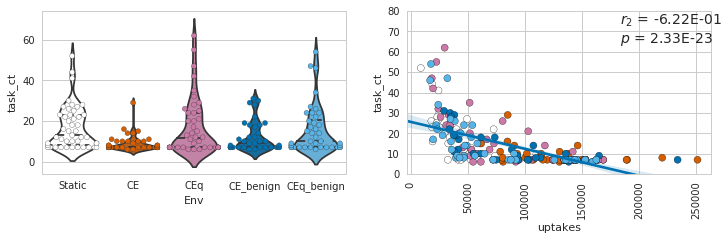
\includegraphics[trim={0 0 0 0}, clip, width=0.75\columnwidth]{figures/LTE/lte-bonus_hgt_vs_task_performance.png}
	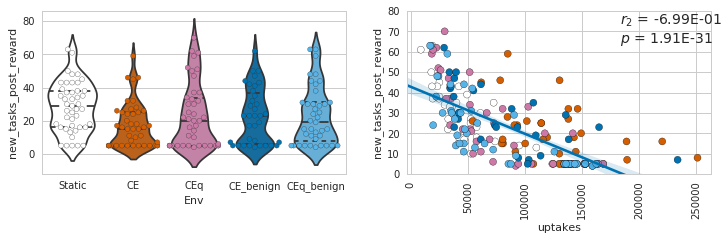
\includegraphics[trim={0 0 0 0}, clip, width=0.75\columnwidth]{figures/LTE/lte-bonus_hgt_vs_task_discovery.png}
	\caption{\textbf{HGT-Bonus vs Task Performance and Discovery}. [TODO DESCRIPTION AND STATS]%
	}
	\label{fig:lte-bonus_hgt_vs_task_performance}
	\end{figure}

%=[FIGURE - complex environment task discovery]
\todo[color=green]{stats}
\todo{caption}
	\begin{figure}[!h]
	%\missingfigure{HGT noBonus vs Task Performance and Discovery}
	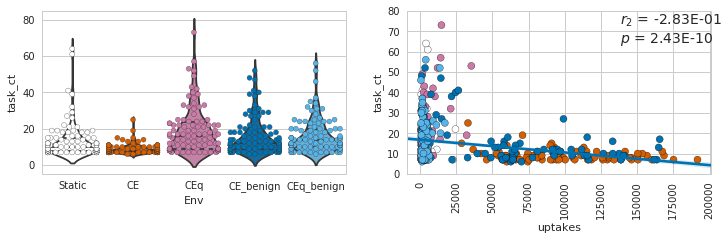
\includegraphics[trim={0 0 0 0}, clip, width=0.75\columnwidth]{figures/LTE/lte-no-bonus_hgt_vs_task_performance.png}
	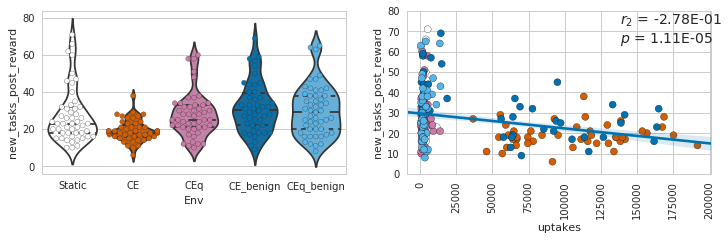
\includegraphics[trim={0 0 0 0}, clip, width=0.75\columnwidth]{figures/LTE/lte-no-bonus_hgt_vs_task_discovery.png}
	\caption{\textbf{HGT-noBonus vs Task Performance and Discovery}. [TODO DESCRIPTION AND STATS]%
	}
	\label{fig:lte-no-bonus_hgt_vs_task_performance}
	\end{figure}	

\subsubsection{Benign changing environments outperform harsh environments in task discovery and task performance in populations with HGT}
Again, consistent with earlier results, populations with HGT follow the same pattern as the earlier experiments. Benign-evolved populations strongly outperform Harsh-evolving in measures of Task Discovery and Task Performance\todo{stats} (Fig.~\ref{fig:lte-hgt_task_performance} and Fig.~\ref{fig:lte-hgt_task_discovery}. These results show that regardless of access to an information rich mutagen, the dominant effect is one of balancing of fitness pressures. 



\section{Conclusion}

%=CE promotes task discovery
Our experiments show that changing environments both directly and indirectly influence long-term evolvability by directly driving exploration across the fitness landscape, and also by creating genetic architectures that increase the rate of new task discovery in novel environments. We hypothesize that these effects are driven by the presence of the accumulated pseudogene-like structures that provide cryptic functionality. In our experiments, the increased rate of task discovery is significant, though relatively small, but we expect that future experiments focused on this specific effect might yield more conclusive results. 

\todo[inline, color=magenta]{fill this in, recapitulating the argument and framing about balancing of fitness effects.}



%%%%%%%%%%%%%%%%%%%%%%%%%%%%%%%%%%%%%%%%%%%%%%%%%%%%%%%%%%%%%%%%%%%%%%%%%%
%%%%%%%%%%%%%%%%%%%%%%%%%%%%%% CHAPTER 6 - CONCLUSION %%%%%%%%%%%%%%%%%%%%
%%%%%%%%%%%%%%%%%%%%%%%%%%%%%%%%%%%%%%%%%%%%%%%%%%%%%%%%%%%%%%%%%%%%%%%%%%


\chapter{Conclusion}
\label{chap:conclusion}
\todo[color=magenta,inline]{FILL THIS IN - Synthesis of all results and how it all fits together to paint a picture of how CE works.}

%=thesis sentence
%=In chapter 2
%=In chapter 3
%=In chapter 4...
This result matches prior research that shows that populations will tend to depress the use of mutagens, even though, in the long-term, higher mutation rates are optimal [CITE].  

%=In chapter 5... 
This result is further evidence that selection tends to act in the short term. Thus, even though certain kinds of mutagens and architectural features may promote long-term evolvability, these features are hitchhiking on short-term adaptive benefits. Thus, our research shows that even though evolvability may evolve, it is not necessarily selected for in the long-term. 

\section{Limitations of Cyclic Changing Environments}
%=CE can be a re-tread, but not as much as feared 
Changing environments produce a set of selective pressures that speed up exploration of genotype space, while also building reservoirs of partial functionality that may be co-opted in the evolution of more complex structures. These features make changing environments useful for both their explanatory power in natural evolution, and as practical tools in the Artificial Life toolkit.
Ultimately, however, cyclic changing environments only re-tread existing phenotypic ground, and though genotypic exploration is faster than under purely directional or stabilizing selection, the space explored remains constrained by the type of phenotypes that are selected. Despite this constraint, however, we see that, particularly under harsh conditions, a lot of novel genotypic ground may be explored, even without direct selection for novelty. 

%=better/different methods
Even so, there must exist methods of exploring genotype space that do not suffer from these limitations at all.
For example, perhaps repeated bottlenecking of populations could promote faster traversal of the fitness landscape in quasi-random directions. More ambitiously, perhaps these kinds of environments could be coupled with dynamically increasing open-ended complexity goals.

%=understanding is vital, conclusion paragraph
\todo{tweak below?}
Understanding the mechanisms by which select environmental conditions alter fitness landscapes is vital to understanding the forces that promote evolvability and increase complexity. In particular, understanding the role of vestigial sites may help us untangle how robustness can promote evolvability. Are these vestigial sites inactive remnants, reservoirs of function, or are they part of a complex compensatory framework supporting and buffering the expression of the phenotype? Or both? Changing environments provide one view into these dynamics, but we must explore further to find other mechanisms for exploring and exploiting genotype space.


\begin{appendices}
%%%%%%%% APPENDIX A
\chapter{Experimentally Deriving Parameters for Changing Environment Cycle Lengths}
\label{appendix:ce_sweep}
Cyclic changing environments have predictable cycles and thus have consistent periods of time that allow adaptation and fixation of traits. Too short a cycle, and traits are not able to fix. Too long a cycle and traits that are no longer selected for in one phase, but are useful in the other, become increasingly vulnerable to loss through genetic drift.

In order to identify an optical cycle time to support our experiments, we surveyed a series of cycle lengths, and measured task performance rates in both benign and harsh changing environments (Fig~\ref{fig:a1-taskexpression}).

%=[FIGURE - complex environment task discovery]
\todo[color=green]{stats}
\todo{caption}
	\begin{figure}[!h]

	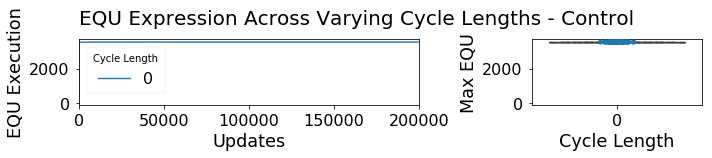
\includegraphics[trim={0 0 0 0}, clip, width=0.75\columnwidth]{figures/A1/a1-taskexpression-control.png}
	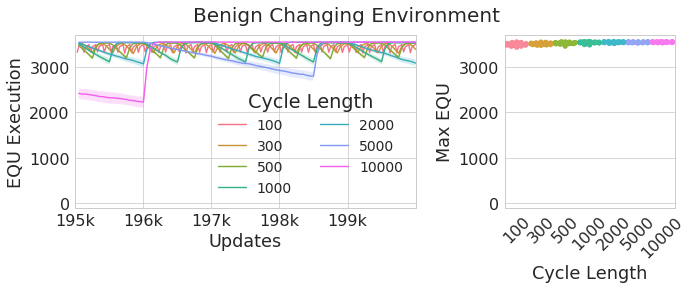
\includegraphics[trim={0 0 0 0}, clip, width=0.75\columnwidth]{figures/A1/a1-taskexpression-benign.png}
	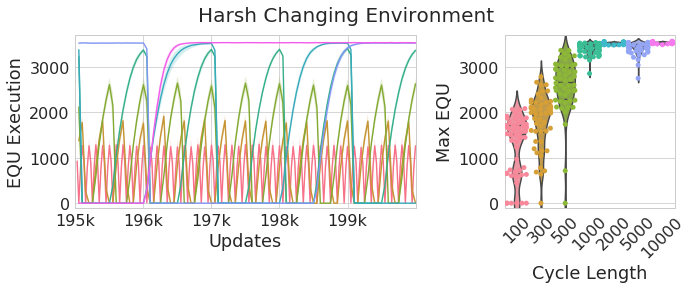
\includegraphics[trim={0 0 0 0}, clip, width=0.75\columnwidth]{figures/A1/a1-taskexpression-harsh.png}
	\caption{\textbf{Survey of task execution} for a series of cycle-lengths. [TODO DESCRIPTION AND STATS]%
	}
	\label{fig:a1-taskexpression}
	\end{figure}

We found that, of our surveyed values, a cycle time of 1,000 updates (roughly 30 generations) both provided adequate time for traits to evolve and fix (and thus be performed by the entire population), but also not enough time for drift to destroy alternate-phase traits, thus minimizing the time required to re-evolve the task. Cycle times that were too short never acquired and fixed adaptive traits in the entire population, while as cycles got longer, the fluctuating tasks would take much longer to re-evolve, indicating that the populations had drifted away from the regions of the mutational landscape that contained them (Fig~\ref{fig:a1-timetofixation}). 

%=[FIGURE - complex environment task discovery]
\todo[color=green]{stats}
\todo{caption}
	\begin{figure}[!h]

	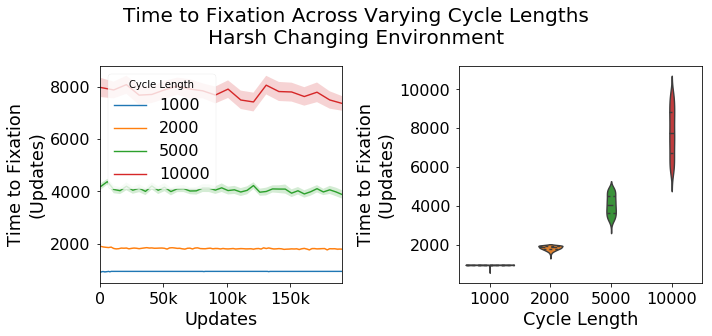
\includegraphics[trim={0 0 0 0}, clip, width=0.85\columnwidth]{figures/A1/a1-timetofixation-harsh.png}
	\caption{\textbf{Survey of task execution} for a series of cycle-lengths. [TODO DESCRIPTION AND STATS]%
	}
	\label{fig:a1-timetofixation}
	\end{figure}

%%%%%%%% APPENDIX B
\chapter{Experimentally Deriving Parameters for HGT Recombination Probability and Bonus Levels}
\label{appendix:hgt_sweep}

\section{Recombination Probability Sweep}
In nature, the probability of horizontal gene transfer occurring varies wildly by species, environmental conditions, and mechanism of action. In order to identify an optimal probability of HGT uptake resulting in recombination, we performed a series of experiments comparing different probabilities, coupled with a pair of basic grazing bonuses. Our initial grazing bonuses were based on the reward given for a similarly complex task - \texttt{NAND} - which only requires a single instruction, plus an \texttt{IO} instruction, to implement. \texttt{NAND} is typically rewarded with a bonus of $2^1$ to execution speed. Thus, performing HGT, which only requires a single instruction - \texttt{HGT-Uptake}, was rewarded similarly.

The goal was to identify a probability of recombination that would, without a grazing bonus, result in a reduced HGT uptake level as compared to with a grazing bonus. Further, we wanted the recombination probability to not be so high as to result in mutational melt-down, thus frequently killing the populations. We found that a level of 0.1 probability met these characteristics. That is, recombination probabilities of less than 0.1 had similar HGT expression rates with and without a bonus, while probabilities above 0.1 tended to have many many fewer surviving populations (Fig~\ref{fig:a2-hgt-probabilitysweep-hgtuse}).

%=[FIGURE - complex environment task discovery]
\todo[color=green]{stats}
\todo{caption}
	\begin{figure}[!h]
	%\missingfigure{$ce-task_performance_by_cycle_length$ harsh}
	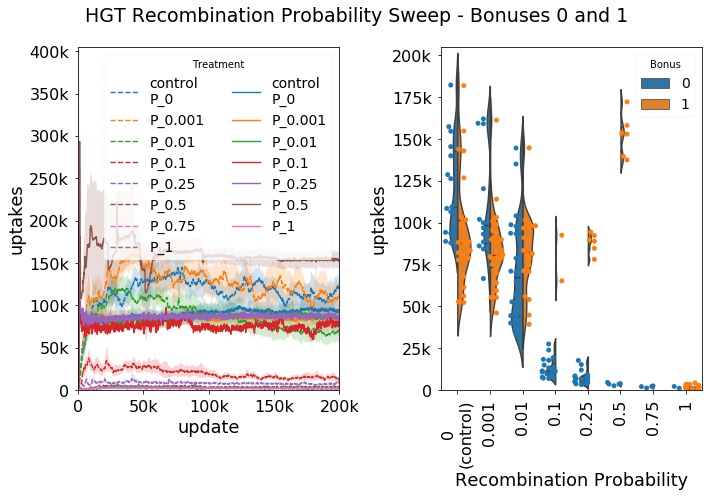
\includegraphics[trim={0 0 0 0}, clip, width=0.85\columnwidth]{figures/A2/hgt-probabilitysweep-hgtuse.png}
	\caption{\textbf{Survey of hgt use} for a series of recombination probabilities. [TODO DESCRIPTION AND STATS]%
	}
	\label{fig:a2-hgt-probabilitysweep-hgtuse}
	\end{figure}


\section{Bonus Sweep}
Similarly, in nature, the amount of nutritive benefit derived from taking up DNA fragments from the environment is difficult to quantify. In Avida, when populations are presented with instructions that provide a direct boost to execution speed, use of these instructions is strongly selected for. Populations rapidly fill their genomes with these instructions, to the exclusion of virtually all else. Thus, our goal in selecting potential bonus levels lay in finding a range of minimal value that would balance the presumably deleterious effects of the HGT uptake instruction, without completely overwhelming the balance of selective pressures we wished to apply to our experiments. As expected, and coupled with the recombination probability above, values around $2^1$ seemed to perform the best (Fig~\ref{fig:a2-hgt-bonussweep-hgtuse}). Above a value of $2^2$, there seem to be diminishing returns.
%=[FIGURE - complex environment task discovery]
\todo[color=green]{stats}
\todo{caption}
	\begin{figure}[!h]
	%\missingfigure{survey of hgt use for a series of bonus values}
	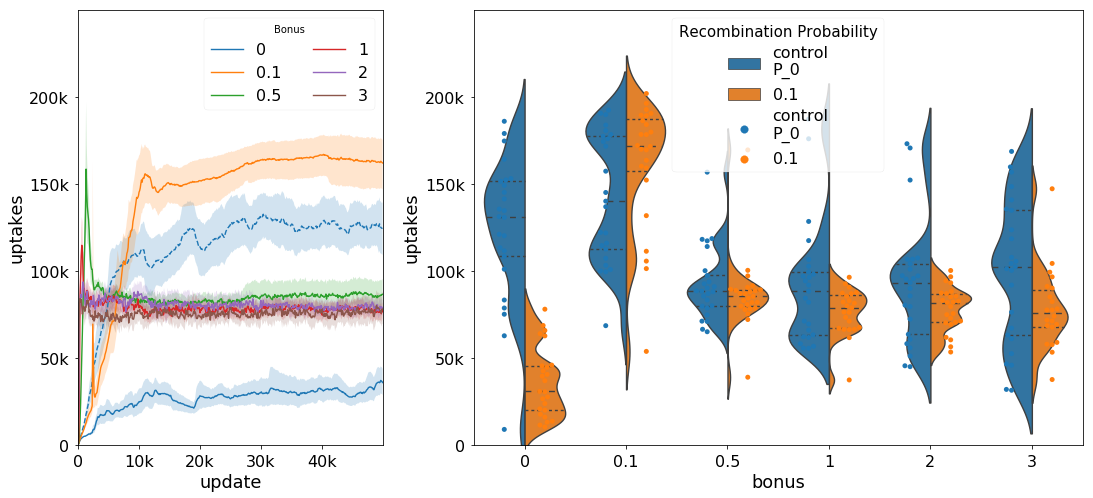
\includegraphics[trim={0 0 0 0}, clip, width=0.85\columnwidth]{figures/A2/a2-hgt-bonussweep-hgtuse.png}
	\caption{\textbf{Survey of task execution} for a series of cycle-lengths. [TODO DESCRIPTION AND STATS]%
	}
	\label{fig:a2-hgt-bonussweep-hgtuse}
	\end{figure}



\section{Comparable Bonus Values}
For later experiments, in order to identify the relationship between HGT uptakes prompted by grazing bonus, and uptakes prompted by evolvability pressures in changing environments, we surveyed a series of bonuses to find a value that, in a static environment, would yield an HGT fragment uptake rate similar to that found in changing environments without a grazing bonus. We found that a bonus value of $2^{0.8}$ yielded similar HGT fragment uptake levels (Fig~\ref{fig:a2-hgt-bonusvsce-hgtuse}).
%=[FIGURE - complex environment task discovery]
\todo[inline]{fix up figure to include CE uptake value, plus less terrible}
\todo[color=green]{stats}
\todo{caption}
	\begin{figure}[!h]
	%\missingfigure{selection of hgt bonus value matching CE no-bonus HGT use}
	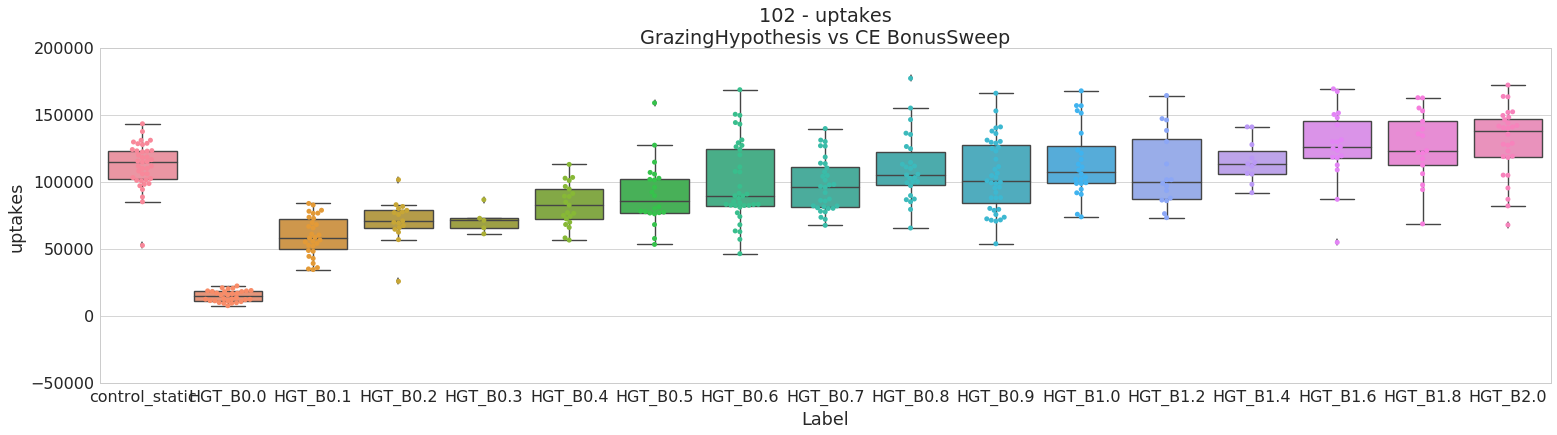
\includegraphics[trim={0 0 0 0}, clip, width=0.85\columnwidth]{figures/A2/a2-hgt-bonusvsce-hgtuse.png}
	\caption{\textbf{Survey of comparable bonus values} for a series of cycle-lengths. [TODO DESCRIPTION AND STATS]%
	}
	\label{fig:a2-hgt-bonusvsce-hgtuse}
	\end{figure}




%%%%%%%% APPENDIX C
\chapter{Changing Environments Elevate All Instruction Use Due to Repeated Bottlenecks}
In Chapter \ref{chap:hgt-preferred}, we observe that the Die mutagen control is also elevated in the changing environments treatment. This counterintuitive effect is due to the repeated bottlenecking of the populations subjected to the harsh changing environment.\ref{fig:bottlenecks}. We observe that under increasingly harsh bottlenecks, rates of execution of the "die" instruction increase to levels comparable to what is seen in the changing environment treatments. Because not all instructions contained in an organism's genome are necessarily executed (due to genetic flow-control structures), it is possible for any instruction to remain dormant. Thus, not all organisms with the "die" instruction in their genome will express it. Thus, the selective pressures of the environmental change may ultimately outweigh that of the die instruction if it is initially dormant in a genome that would survive a harsh environmental change and reproduce. 

\todo{rework figure}
\todo[color=green]{stats}
\todo{caption}
\begin{figure}[h!]
\begin{center}
\includegraphics[width=0.7\columnwidth]{figures/HGT/die_bottleneck.png}
\caption{bleh
}\label{fig:bottlenecks}
\end{center}
\end{figure}

\end{appendices}


\backmatter
\makebibliographypage
\SingleSpacing
\bibliography{dis}
\bibliographystyle{unsrt}
\end{document}